\documentclass[review]{elsarticle}

\usepackage{lineno,hyperref}

\usepackage{latexsym,amsthm,amsmath,amssymb,mathrsfs,dsfont,upgreek,stackengine,graphicx,caption, float,enumerate}
\usepackage{pdfpages,courier,subcaption,inputenc,tikz,verbatim,blkarray, listings,latexsym,pythonhighlight,xcolor,geometry,xparse}
\usepackage{algorithmic}

\newcommand{\code}[1]{\colorbox{light-gray}{\texttt{#1}}}

\usepackage[ruled,vlined]{algorithm2e}


\newtheorem{remark}{Remark}
\newtheorem{theorem}{Theorem}

\modulolinenumbers[5]

\journal{Journal of Computational Physics}

\geometry{a4paper,left=2cm,right=2cm,top=1cm,bottom=1.5cm}



%%%%%%%%%%%%%%%%%%%%%%%
%% Elsevier bibliography styles
%%%%%%%%%%%%%%%%%%%%%%%
%% To change the style, put a % in front of the second line of the current style and
%% remove the % from the second line of the style you would like to use.
%%%%%%%%%%%%%%%%%%%%%%%

%% Numbered
%\bibliographystyle{model1-num-names}

%% Numbered without titles
%\bibliographystyle{model1a-num-names}

%% Harvard
%\bibliographystyle{model2-names.bst}\biboptions{authoryear}

%% Vancouver numbered
%\usepackage{numcompress}\bibliographystyle{model3-num-names}

%% Vancouver name/year
%\usepackage{numcompress}\bibliographystyle{model4-names}\biboptions{authoryear}

%% APA style
%\bibliographystyle{model5-names}\biboptions{authoryear}

%% AMA style
%\usepackage{numcompress}\bibliographystyle{model6-num-names}

%% `Elsevier LaTeX' style
\bibliographystyle{elsarticle-num}
%%%%%%%%%%%%%%%%%%%%%%%

\begin{document}

\begin{frontmatter}

\title{Numerical aspects of Casimir energy computation in acoustic and electromagnetic scattering}
%\tnotetext[mytitlenote]{Fully 	documented templates are available in the elsarticle package on \href{http://www.ctan.org/tex-archive/macros/latex/contrib/elsarticle}{CTAN}.}

%% Group authors per affiliation:
\author[mymainaddress]{Timo Betcke}
\ead[url]{t.betcke@ucl.ac.uk}
\address[mymainaddress]{Department of Mathematics, University College London, London, WC1E 6BT, UK}


\author[mysecondaryaddress]{Alexander Strohmaier}
\ead[url]{a.strohmaier@leeds.ac.uk}
\address[mysecondaryaddress]{School of Mathematics, University of Leeds, Leeds, LS2 9JT, UK}

%% or include affiliations in footnotes:
\author[mymainaddress]{Xiaoshu Sun\corref{mycorrespondingauthor}}
\cortext[mycorrespondingauthor]{Corresponding author}
\ead[url]{xiaoshu.sun.18@ucl.ac.uk}



\begin{abstract}
    Computing the Casimir energy is a classical problem of quantum electrodynamics going back to the 1940s. In the early two thousands a significant breakthrough
     was achieved by representing the Casimir energy as the computation of the integral of the log determinant of certain boundary integral operators in the complex plane. 
Recently, this log determinant formula was investigated in the context of the Krein spectral shift function, which suggests a potential alternative computational 
approach based on the numerical evaluation of scattering matrices. In this paper, we will give an overview of these computational techniques of computing 
the Casimir energy in three dimensional acoustic scattering. Afterwards, we will discuss the spectral properties of the block matrices 
inside the formula of the Casimir energy, which are constructed by the integral operators and investigate how to use these properties to speed up Casimir computations for large-scale practical problems.
\end{abstract}

\begin{keyword}
Krein spectral shift function \sep Casimir energy \sep Krylov subspace \sep inverse-free generalized eigenvalue problem \sep Bempp
\end{keyword}

\end{frontmatter}

%\linenumbers
\section{Introduction}\label{Introduction}
Casimir interactions are forces between objects such as perfect conductors. Hendrik Casimir predicted and computed this effect in the special case of two planar 
conductors in 1948 using a divergent formula for the zero point energy and applying regularisation to it \cite{casimir1948attraction}. This resulted in the 
famous formula for the attractive Casimir force per unit area 
\begin{align*}
    F(a) = -\frac{1}{A}\frac{\partial \mathcal{E}}{\partial a} = -\frac{\hbar c\pi^{2}}{240a^{4}},
\end{align*}
between two perfectly conducting plates, where $A$ is the cross-sectional area of the boundary plates and $\mathcal{E}$ is the Casimir energy as 
computed from a zeta regularised mode sum. The result here is for the electromagnetic field which differs by a factor of two from the force resulting from a 
massless scalar field.
This force was measured experimentally by Sparnaay 
about 10 years later \cite{sparnaay1958measurements} and the Casimir effect has since become famous for its intriguing derivation and its counterintuitive nature.
In 1996, precision measurements of the Casimir force between 
 extended bodies were conducted by S.K. Lamoreaux \cite{lamoreaux1997demonstration}  confirming the theoretical predictions including corrections for 
realistic materials. From 2000 to 2008, the Casimir force has been measured in various 
experimental configurations, such as cylinder-cylinder \cite{ederth2000template}, plate-plate \cite{bressi2002measurement}, 
sphere-plate \cite{krause2007experimental} and sphere-comb \cite{chan2008measurement}. 
The presence of the Casimir force has also been quoted as evidence for the zero point energy of the vacuum having direct physical significance.
The classical way to compute Casimir forces mimicks Casimir's original computation and is based on zeta function regularisation of the vacuum energy. 
This has been carried out for a number of particular geometric situations (see \cite{bordag2001new, bordag2009advances, elizalde1989expressions, elizalde1990heat, kirsten2001spectral} and references therein). 
The derivations are usually based on special functions and their properties and require explicit knowledge of the spectrum of the Laplace operator.

In 1960s, Lifshitz and collaborators extended and modified this theory to the case of dielectric media \cite{dzyaloshinskii1961general} 
gave derivations based on the stress energy tensor. It has also been realised by quantum field theorists  
(see e.g. \cite{brown1969vacuum, dzyaloshinskii1961general, deutsch1979boundary, kay1979casimir, scharf1992casimir}) with various degrees of mathematical rigour that 
the stress energy approach yields Casimir's formula directly without the need for renormalisation or artificial regularisation.
This tensor is defined by comparing the induced vacuum states of the quantum field with boundary conditions and the free theory. 
Once the renormalised stress energy tensor is mathematically defined, the computation of the Casimir energy density becomes a problem of spectral 
geometry (see e.g. \cite{fulling2007vacuum}). The renormalised stress energy tensor and its relation to the Casimir effect can be understood at the 
level of rigour of axiomatic algebraic quantum field theory. We note however that the computation of the local energy density is non-local and requires 
some knowledge of the spectral resolution of the Laplace operator, the corresponding problem of numerical analysis is therefore extremely hard.

Lifshitz and collaborators also offered an alternative description based on the van der Waals forces between molecules.
The plates consist of a collection of atomic-scale electric dipoles randomly oriented in the absence of the external forcing field. Quantum and thermal 
fluctuations may make the dipoles align spontaneously, resulting in a net electric dipole moment. The dipoles in the opposite plate feel this field
across the gap and align as well. The two net electric dipole moments make the two plates attract each other. This approach emphasizes the 
influence from the materials more than the fluctuations in the empty space between the plates.

Somewhat independently from the spectral approach determinant formulae based on the van der Waal's mechanism were derived by various authors. 
We note here Renne \cite{renne1971microscopic} who gives a determinant formula for the van der Waals force based on microscopic considerations. Various other authors 
give path-integral considerations based on considerations of surface current fluctuations 
\cite{bimonte2017nonequilibrium, emig2007casimir, emig2006casimir, EGJK2008, emig2008casimir, kenneth2006opposites, kenneth2008casimir, milton2008multiple, rahi2009scattering}. The final formulae proved suitable for numerical schemes 
and were also very useful to obtain asymptotic formulae for Casimir forces for large and small separations. The mathematical relation between the various 
approaches remained unclear, with proofs of equality only available in special cases.
A full mathematical justification of the determinant formulae as the trace of an operator describing the Casimir energy was only recently achieved in 
\cite{MR4484208} for the scalar field and \cite{strohmaier2021classical} for the electromagnetic field. It was also proved recently in \cite{fang2021mathematical} that the 
formulae arising from Zeta regularistation, from the stress energy tensor, and from the determinant of the single layer operator all give the same Casimir forces.

We will now describe the precise mathematical setting and review the theory.
Let $\Omega \subset \mathbb{R}^{d}$ be a non-empty bounded open subset with Lipschitz boundary $\partial \Omega$, which is the union of connected open 
sets $\Omega_{j}$, for $j = 1, \dots, N$. We assume that the complement $\mathbb{R}^{d} \backslash \Omega$ of $\Omega$ is connected and the closures of $\Omega_{j}$ 
are pairwise non-intersecting.
We denote the  $N$ connected components of the boundary $\partial\Omega$ by $\partial\Omega_{j}$. 
We will think of the open set $\Omega$ as a collection of objects $\Omega_{j}$ placed in $\mathbb{R}^{d}$ and will refer to them as {\sl obstacles}.

Then, several unbounded self-adjoint operators densely defined in $L^{2}(\mathbb{R}^{d})$
can be defined.
\begin{itemize}
    \item The operator $\Delta$ is the Laplace operator with Dirichlet boundary conditions on $\partial\Omega$.
    \item For $j = 1, \dots, N$, the operator $\Delta_{j}$ is the Laplace operator with Dirichlet boundary conditions on $\partial\Omega_{j}$.
    \item The operator $\Delta_{0}$ is the ``free'' Laplace operator on $\mathbb{R}^{d}$ with domain $H^{2}(\mathbb{R}^{d})$.
\end{itemize}

These operators contain the dense set $C^\infty_0(\mathbb{R}^d \setminus \partial \Omega)$ in their domains.
If $f: \mathbb{R} \to \mathbb{R}$ is a polynomially bounded function this set is also contained in the domain of the operators
$f(\Delta^{\frac{1}{2}}), f(\Delta_{j}^{\frac{1}{2}})$, and $f(\Delta_{0}^{\frac{1}{2}})$, in particular the operator
$$
 D_{f} = f(\Delta^{\frac{1}{2}}) - f(\Delta_{0}^{\frac{1}{2}}) - \left(\sum_{j = 1}^{N}[f(\Delta_{j}^{\frac{1}{2}}) - f(\Delta_{0}^{\frac{1}{2}})]\right)
$$
is densely defined. It was shown in \cite{MR4484208} that under additional analyticity assumptions on $f$ the operator
$D_{f}$ is bounded and extends by continuity to a trace-class operator on $L^2(\mathbb{R}^{d})$. 
These analyticity assumptions are in particular satisfied by $f(k) = (k^{2}+ m^{2})^{\frac{s}{2}}$ for any $s > 0, m \geq 0$ and one has
\begin{align}\label{trace formula in terms of the boundary op}
    \text{Tr}\left( D_{f} \right)  = \frac{s}{\pi} \sin\left(\frac{\pi}{2} s\right) \int_{m}^{\infty} k (k^{2} + m^{2})^{\frac{s}{2}-1}\Xi(\mathrm{i} k) dk,
\end{align}
where the function $\Xi$ is given by
$$
 \Xi(k) = \log \det V_{k} \tilde V_{k}^{-1}
$$
and the operators $V_{k}$ and $\tilde V_{k}$ are certain boundary layer operators that will be defined later. 
It was proved in  \cite{MR4484208} that the above determinant is well-defined in the sense of Fredholm as the operator $V_{k} \tilde V_{k}^{-1}$ near the positive imaginary axis differs
from the identity operator by a trace-class operator on the Sobolev space $H^\frac{1}{2}(\partial \Omega)$.
We remark here that the paper \cite{MR4484208} assumed the boundary to be smooth and the operators $V_k  \tilde V_k^{-1}$ was considered as a 
map on $L^2(\partial \Omega)$. The main result of the paper also holds for Lipschitz boundaries if $L^2(\partial \Omega)$ is replaced by $H^\frac{1}{2}(\partial \Omega)$. This requires minor modifications of the proof but we will not discuss this further here, as we are now focusing on computational aspects.

We also recall that by the Birman-Krein formula we have for any even function $h \in \mathcal{S}(\mathbb{R})$ the equality
\begin{align}\label{B-K formula}
    \text{Tr}\left(h(\Delta^{\frac{1}{2}}) - h(\Delta_{0}^{\frac{1}{2}}) - \left(\sum_{j = 1}^{N}[h(\Delta_{j}^{\frac{1}{2}}) - h(\Delta_{0}^{\frac{1}{2}})]\right)\right)  = \int_{0}^{\infty}h'(k)\xi(k)dk,
\end{align}
where 
\begin{align*}
    \xi(k) = \frac{1}{2\pi \mathrm{i}}\log\left(\frac{\det(S(k))}{\det(S_{1,k})\cdots\det(S_{N,k}(k))}\right)
\end{align*}
will be called the relative Krein spectral shift function. Here, $S_{j,k}$ are the scattering matrices of $\Delta_{j}$ associated to the objects $\Omega_{j}$. Note here that the class of functions for which this is true can be relaxed to a certain extent, but even the most general version does not allow unbounded functions such as $f(k)$ with $s>0, m\geq 0$.
The relative spectral shift function can however be related via a Laplace transform to the Fourier transform of the relative spectral shift function (see \cite{MR4396069}). Under mild convexity assumptions this can be connected to the Duistermaat-Guillemin trace formula in obstacle scattering theory to give an asymptotic expansion of  $\Xi(k)$ 
in terms of the minimal distance $\delta>0$ between the obstacles and the linearised Poincar\'e map of the bouncing ball orbits between the obstacles of that length. One has
$$
 \Xi(k) =- \sum_{j} \frac{1}{|\det(I - P_{\gamma_j})|^{\frac{1}{2}}} e^{2 i \delta k} + o(e^{- 2 \delta \text{Im}{k}}),
$$
where the sum is over  bouncing ball modes of length $2 \delta$ and $P_{\gamma_j}$ is the associated Poincar\'e map, where $\gamma_{j}$ is the shortest bouncing ball orbits. 

The Casimir energy of the configuration $\Omega$ for a massless scalar field would then be given by $D_f$ in the case when $f(k)=k$ and is therefore equal to
$$
\zeta = \frac{\hbar c}{2 \pi} \int _{0}^{\infty} \Xi(\mathrm{i}k) dk.
$$

In this paper, we are going to introduce the numerical framework of computing the Casimir energy based on the evaluation of the log determinant of the integral 
operators in the acoustic case \footnote{The mathematical theories and numerical experiments in the Maxwell case have been done as well and they will be 
reported in another paper.} in Section \ref{Numerical methods for computing the Casimir energy}. Afterwards,
two efficient methods for computing the integrand of the Casimir energy will be illustrated in Section \ref{Krylov subspace for generalized eigenvalue problem}
which makes us compute the large-scale problem efficiently. In Section \ref{Numerical experiments}, several examples on computing the Casimir energy between 
 compact objects will be shown and we will also compare our results with others computed in other methods. Note that all the tests and examples in this paper were computed 
with version 0.2.4 of the Bempp-cl library \cite{scroggs2017software}. Finally, Section \ref{Conclusion} will conclude 
our paper and discuss the future plan as well.

% and discuss the spectral properties 
% of the block matrices constructed from the integral operators in Section \ref{Spectral property of the integral operators}.

\section{Numerical methods for computing the Casimir energy  in acoustic scattering}\label{Numerical methods for computing the Casimir energy}
% !TEX root =  main.tex

In this section, we give details of computing the Casimir energy via boundary integral operator discretisations. 
Assume 
$\Omega^{-}\subset \mathbb{R}^{d}$, for $d \geq 2$ is the interior open bounded domain that the scatterer occupies with piecewise smooth Lipschitz boundary $\Gamma$. The exterior domain is denoted as 
$\Omega^{+} = \mathbb{R}^{d}\backslash\overline{\Omega^{-}}$. $\boldsymbol{n}$ is the almost everywhere defined exterior unit normal to the surface $\Gamma$ pointing outwards from $\Omega^{-}$ and 
$\boldsymbol{n}_{\boldsymbol{x}}$ is normal to $\Gamma$ at the point $\boldsymbol{x}\in\Gamma$.

In the scalar case, the Casimir energy can be expressed in terms of certain single-layer boundary operator, which we will define below. We then present its relationship with the Krein-Spectral shift function and demonstrate how it can practically be computed.

\subsection{The single-layer boundary operator}
For the bounded interior domain $\Omega^{-}$ or the unbounded exterior domain $\Omega^{+}$, the space of the (locally) square integrable functions is 
\begin{align*}
    L^{2}(\Omega^{-}) &:= \left\{f:\Omega^{-}\rightarrow\mathbb{C}, f \text{ is Lebesgue measurable and} \int_{\Omega^{-}}|f|^{2} < \infty \right\},\\
    L_{\text{loc}}^{2}(\Omega^{+}) &:= \left\{f:\Omega^{+}\rightarrow\mathbb{C},\ f \text{ is Lebesgue measurable and} \int_{K}|f|^{2} < \infty, \ \text{for all compact}\ K \subset \overline{\Omega^{+}} \right\}
\end{align*}
and note that the subscript ``loc'' can be removed if the domain is bounded (i.e. $L_{\text{loc}}^{2}(\Omega^{-}) = L^{2}(\Omega^{-})$).
We denote by $H_{\text{loc}}^{s}(\Omega^{\pm})$ the standard Sobolev spaces associated with the Lipschitz domains. In particular, for integers $s\geq 0$, we have 
\begin{align*}
    H_{\text{loc}}^{s}(\Omega^{\pm}):=\left\{f\in L_{\text{loc}}^{2}(\Omega^{\pm}), \forall\alpha \text{ s.t.} |\alpha|\leq s, D^{\alpha}f\in L_{\text{loc}}^{2}(\Omega^{\pm})\right\},
\end{align*}
where $\alpha = (\alpha_{1}, \alpha_{2}, \dots, \alpha_{d})$ is a multi-index and $|\alpha| = \alpha_{1} + \alpha_{2} + \dots + \alpha_{d}$, and 
the derivative is defined in the weak sense.
One also has the Sobolev spaces on the boundary $H^{s}(\Gamma)$ for any $-\frac{1}{2} \leq s \leq \frac{1}{2}$.
For a function $p$ on $\Omega$ that is continuous on the boundary we have the trace map $\gamma_{D}^{\pm}$ defined by
\begin{align*}
    \gamma_{\text{D}}^{\pm}p(\boldsymbol{x}):=\lim_{\Omega^{\pm}\ni\boldsymbol{x'}\rightarrow\boldsymbol{x}\in\Gamma}p(\boldsymbol{x'})
\end{align*}
that maps the function to its boundary value. This trace map is well-known to extend continuously to a map
$\gamma_{D}^{\pm}:  H_{\text{loc}}^1(\Omega) \to H^{1/2}(\Gamma) $. For the purposes of this paper it is sufficient to understand $H^{1/2}(\Gamma)$ as range space of the trace operator on $H_{\text{loc}}^1(\Omega)$ . We also need the space $H^{-1/2}(\Gamma)$, which is the dual space of $H^{1/2}(\Gamma)$ with $L^2(\Gamma)$ as pivot space.

We can now define the single-layer boundary $V_{k}:H^{-1/2}(\Gamma)\rightarrow H^{1/2}(\Gamma)$ as the continuous extension of the map defined in terms of an integral kernel as follows

\begin{align*}
    (V_{k}\mu)(\boldsymbol{x}) := \int_{\Gamma}g_{k}(\boldsymbol{x},\boldsymbol{y})\psi(\boldsymbol{y})dS_{\boldsymbol{y}}, \ \ \ \ \ 
    \text{for}\ \mu\in H^{-\frac{1}{2}}(\Gamma) \  \text{and} \ \boldsymbol{x}\in\Gamma.
\end{align*}
Here, 
\begin{align}\label{Green's function}
    g_{k}(\boldsymbol{x},\boldsymbol{y}) = \begin{cases}
          \frac{\mathrm{i}}{4}H_{0}^{(1)}(k|\boldsymbol{x}-\boldsymbol{y}|), \ \ \ \ &\text{for} \ d = 2\\
          \frac{e^{ik|\boldsymbol{x}-\boldsymbol{y}|}}{4\pi|\boldsymbol{x} - \boldsymbol{y}|}, \ \ \ \ &\text{for} \ d = 3,
        \end{cases}
\end{align}
with $H_{0}^{(1)}$  a Hankel function of the first kind.



\subsection{The formula of the Casimir energy}
% By \cite{MR4484208}, the Krein spectral shift function is defined as 
% \begin{align*}
%     \xi(k) = \frac{1}{2\pi \mathrm{i}}\log\left(\frac{\det(S(k))}{\det(S_{1,k})\cdots\det(S_{N,k})}\right),
% \end{align*}
% where $S_{i,n}$ is the scattering matrix associated with the $n$th scatterer. These scattering matrices can be constructed  $S_{i,n} = I + 2T_{i,n}$, where 
% $I$ is the identity matrix and $T_{i,n}$ is the $T$-matrix. The method of computing the $T$-matrix is fully discussed in \cite{waterman1969new} and 
% \cite{ganesh2008far}.
Before we present the formula of the Casimir energy, let us introduce the following theorem.
\begin{theorem}\cite{MR4484208}
    Consider $\Omega$ as a domain assembling from individual objects $\Omega_{i}$. Let $V_{k}$ be the single-layer boundary operator defined on the boundary 
    $\partial\Omega = \bigcup_{i = 1}^{N}\partial\Omega_{i}$, and $\tilde{V}_{k}$ is the ``diagonal part'' of $V_{k}$ by restricting the integral 
    kernel to the subset $\bigcup_{i = 1}^{N}\partial\Omega_{i}\times\partial\Omega_{i}\subset\partial\Omega\times\partial\Omega$ then the operator 
    $V_{k}\tilde{V}_{k}^{-1} - I$ with $I$ the identity operator is trace-class and 
    \begin{align*}
        \Xi(k) = \log\det\left(V_{k}\tilde{V}_{k}^{-1}\right),
    \end{align*}
    where the Fredholm determinant $\det(V_{k}\tilde{V}_{k}^{-1})$ is well-defined 
    \footnote{The Fredholm determinant is a generalization of a determinant of finite dimensional matrix to finite dimensional linear operator 
    which differ from the identity operator by a trace class operator \cite[Section 6.5.2]{MR2300779}. Since the operator $V_{k}\tilde{V}_{k}^{-1} - I$ 
    with $I$ the identity operator is trace-class in the close upper half space \cite[Theorem 1.7]{MR4484208}, the determinant $\det(V_{k}\tilde{V}_{k}^{-1})$ is well-defined.}.
   and by taking $m = 0$ and $s = 1$ in \eqref{trace formula in terms of the boundary op}, this gives the formula 
    \begin{align}\label{slp and matrix}
        \emph{\text{Tr}}\left(\Delta^{\frac{1}{2}} + (N - 1)\Delta_{0}^{\frac{1}{2}} - \sum_{i = 1}^{N}\Delta_{j}^{\frac{1}{2}}\right)  =  \frac{1}{\pi}\int_{0}^{\infty}\Xi(\mathrm{i}k)dk.
    \end{align}
\end{theorem}

Equation \eqref{slp and matrix} is used to compute the Casimir energy between the objects and the formula is written as
\begin{align}\label{KSSF and CasE}
    \zeta = \frac{\hbar c}{2\pi}\int_{0}^{\infty}\Xi(\mathrm{i}k)dk.
\end{align}
This formula is identical to the one proposed by Johnson in \cite{reid2009efficient} who uses a non-rigorous path integral argument for its derivation.

\begin{remark}
    There is a relation between the relative Krein spectral shift function and the single-layer boundary integral operator. That is,
    for $k > 0$, 
    \begin{align*}
        -\frac{1}{\pi}\emph{\text{Im}}\,\Xi(k) = \frac{\mathrm{i}}{2\pi}(\Xi(k) - \Xi(-k)) = \xi(k).
    \end{align*}
\end{remark}
% \begin{remark}
%     Note that the integral $\frac{\hbar c}{2}\int_{0}^{\infty}\xi(k)dk$ in \eqref{KSSF and CasE} is not Lebesgue convergent and requires regularisation for its numerical evaluation. The right-hand side integral does not suffer from this issue.
% \end{remark}

% {\color{red} Corrected to here}


\subsection{Galerkin discretization and boundary element spaces}
In order to compute the integral \eqref{KSSF and CasE}, we need to compute the log determinant of the operators $V_{k}\tilde{V}_{k}^{-1}$. In this section we discuss Galerkin discretisations to compute this quantity.

Define the 
triangulation $\mathcal{T}_{h}$ of the boundary surface $\Gamma$ with triangular surface elements $\tau_{l}$ and associated nodes $\boldsymbol{x}_{i}$ 
s.t. $\overline{\mathcal{T}_{h}} = \bigcup_{l}\overline{\tau_{l}}$, where $h$ is the mesh size and define the space of the continuous piecewise linear functions
\begin{align*}
    P_{h}^{1}(\Gamma) = \{v_{h}\in C^{0}(\Gamma): v_{h}|_{\tau_{l}}\in\mathbb{P}_{1}(\tau_{l}), \ \text{for} \ \ \tau_{l}\in\mathcal{T}_{h}\},
\end{align*}
where $\mathbb{P}_{1}(\tau_{l})$ denotes the space of polynomials of order less than or equal to 1 on $\tau_{\ell}$. We have

\begin{align*}
    P_{h}^{1}(\Gamma) := \text{span}\{\phi_{j}\} \subset H^{-\frac{1}{2}}(\Gamma)
\end{align*}
with 
\begin{align*}
    \phi_{j}(\boldsymbol{x}_{i}) = \begin{cases}
        1, & i = j,\\
        0, & i\neq j
    \end{cases}
\end{align*}
being the nodal basis functions.

\begin{remark}
Since $H^{-1/2}(\Gamma)$ does not require continuity we could use a space of simple piecewise constant functions. The reason why we choose piecewise linear functions is the size of the arising matrix systems for dense calculations. The computation of the log-determinant requires $\mathcal{O}(n^3)$ operations, where $n$ is the dimension of our approximation basis. For sphere-like and other similar geometries there are in practice roughly twice as many triangles as nodes in the mesh. Hence, while the assembly cost with piecewise linear functions is higher, the resulting matrix has only half the dimension, resulting in roughly a factor eight reduction of computational complexity for the log determinant. A disadvantage is that on geometries with corners or edges the converges close to these singularities is suboptimal with continuous piecewise linear functions.
\end{remark}

Having defined the basis function $\phi_j$, we can represent each element inside the Galerkin discretization form. Assume there are $N$ objects,
then the matrix of the operator $V_k$ is an $N$ by $N$ block matrix, written as 
\begin{align}\label{matrix V}
    \mathsf{V}(k) = \begin{bmatrix}
        \mathsf{V}_{11}(k) & \mathsf{V}_{12}(k) & \cdots & \mathsf{V}_{1N}(k) \\
        \mathsf{V}_{21}(k) & \mathsf{V}_{22}(k) & \cdots & \mathsf{V}_{2N}(k) \\
        \vdots & \vdots & \ddots & \vdots \\
        \mathsf{V}_{N1}(k) & \mathsf{V}_{N2}(k) & \cdots & \mathsf{V}_{NN}(k) \\
\end{bmatrix}
\end{align}
and the matrix $\tilde{V}_{k}$ is the diagonal part of $V_{k}$:
\begin{align}\label{matrix tilde V}
    \tilde{\mathsf{V}}(k) = \begin{bmatrix}
        \mathsf{V}_{11}(k) & 0      & \cdots & 0 \\
    0      & \mathsf{V}_{22}(k) & \cdots & 0\\
    \vdots & \vdots & \ddots & \vdots \\
    0      & 0      & \cdots & \mathsf{V}_{NN}(k) \\
\end{bmatrix}.
\end{align}
Therefore, the element in the $m$th row and $n$th column of the block matrix $\mathsf{V}_{ij}(k)$ is 
\begin{align}\label{Elements in matrix V}
    \mathsf{V}_{ij}^{(m,n)} (k) = \langle V_{ij}(k)\phi_{n}^{(j)}, \phi_{m}^{(i)}\rangle = 
    \int_{\Gamma_{j}}\phi_{m}^{(i)}(\boldsymbol{x})\int_{\Gamma_{i}}g_{k}(\boldsymbol{x}, \boldsymbol{y})\phi_{n}^{(j)}(\boldsymbol{y})dS_{\boldsymbol{y}}dS_{\boldsymbol{x}},
\end{align}
where $\boldsymbol{\phi}^{(i)} = \begin{bmatrix}
    \phi_{1}^{(i)} & \phi_{2}^{(i)} & \dots & \phi_{N}^{(i)}
\end{bmatrix}$ is the set of basis functions defined on the $i$th object and $\langle \cdot, \cdot \rangle$
denotes the standard $L^{2}(\Gamma)$ inner product.


The value of $\Xi(\mathrm{i}k) = \log\det(\mathsf{V}(\mathrm{i}k)\tilde{\mathsf{V}}(\mathrm{i}k)^{-1})$ can now be explicitly computed by evaluating the corresponding log determinants.

The function $\Xi(\mathrm{i}k)$ has a very favourable decay behaviour for growing $k$ that we can use to limit the number of quadrature points necessary to evaluate the corresponding Casimir integral, namely under certain convexity assumptions on the obstacles it holds that
$$
\Xi(\mathrm{i}k) = \mathcal{O}(e^{-2Zk}).
$$
Here, $Z$ is the minimum distance between the obstacles  \cite[Theorem 4.1]{fang2022trace}.

This result can be justified heuristically, using a simple matrix perturbation argument. Consider a symmetric matrix $A$ partitioned as
$$
A = \begin{bmatrix}A_1 & 0\\
                              0   & A_2
       \end{bmatrix}.
$$
and a symmetric matrix $E$ partitioned as
$$
E= \begin{bmatrix}0 & E_1^T\\
     E_1 & 0
     \end{bmatrix}
$$
Then it holds for the $i$th eigenvalue $\lambda_i(A)$ and the $i$th eigenvalue $\lambda_i(A+E)$ that
$$
|\lambda_i(A) - \lambda_i(A+E)| \leq \frac{\|E\|^2}{\text{gap}_i},
$$
where $\text{gap}_i$ is the distance of $\lambda_i(A)$ to the spectrum of $A_2$ if $\lambda_i(A)$ is an eigenvalue of $A_1$, and to the spectrum of $A_1$ if $\lambda_i(A)$ is an eigenvalue of $A_2$. Details can be found in  
\cite{mathias1998quadratic}.
% {\color{red} The reference to Roy Matthias is suddenly missing}.

Now assume that we have two different obstacles. Then we have $A_1 = \mathsf{V}_{11}(\mathrm{i}k)$, $A_2 = \mathsf{V}_{22}(\mathrm{i}k)$ and $E_1 = \mathsf{V}_{21}(\mathrm{i}k)$ as the matrix of cross interactions 
between the two obstacles. For complex wavenumbers $\mathrm{i}k$, the Green's function between two obstacles decays exponentially like $e^{-Zk}$, where $Z$ is the minimal distance between them, 
resulting in a matrix perturbation result of the form $|\lambda_i(\mathsf{V}) - \lambda_i(\tilde{\mathsf{V}})| = O(e^{-2Zk})$ for increasing $k$ (see Figure \ref{Distinct:The integrand decays exponentially}
), from which the corresponding perturbation result for the log determinant follows.

\begin{figure}[H]
    \centering
    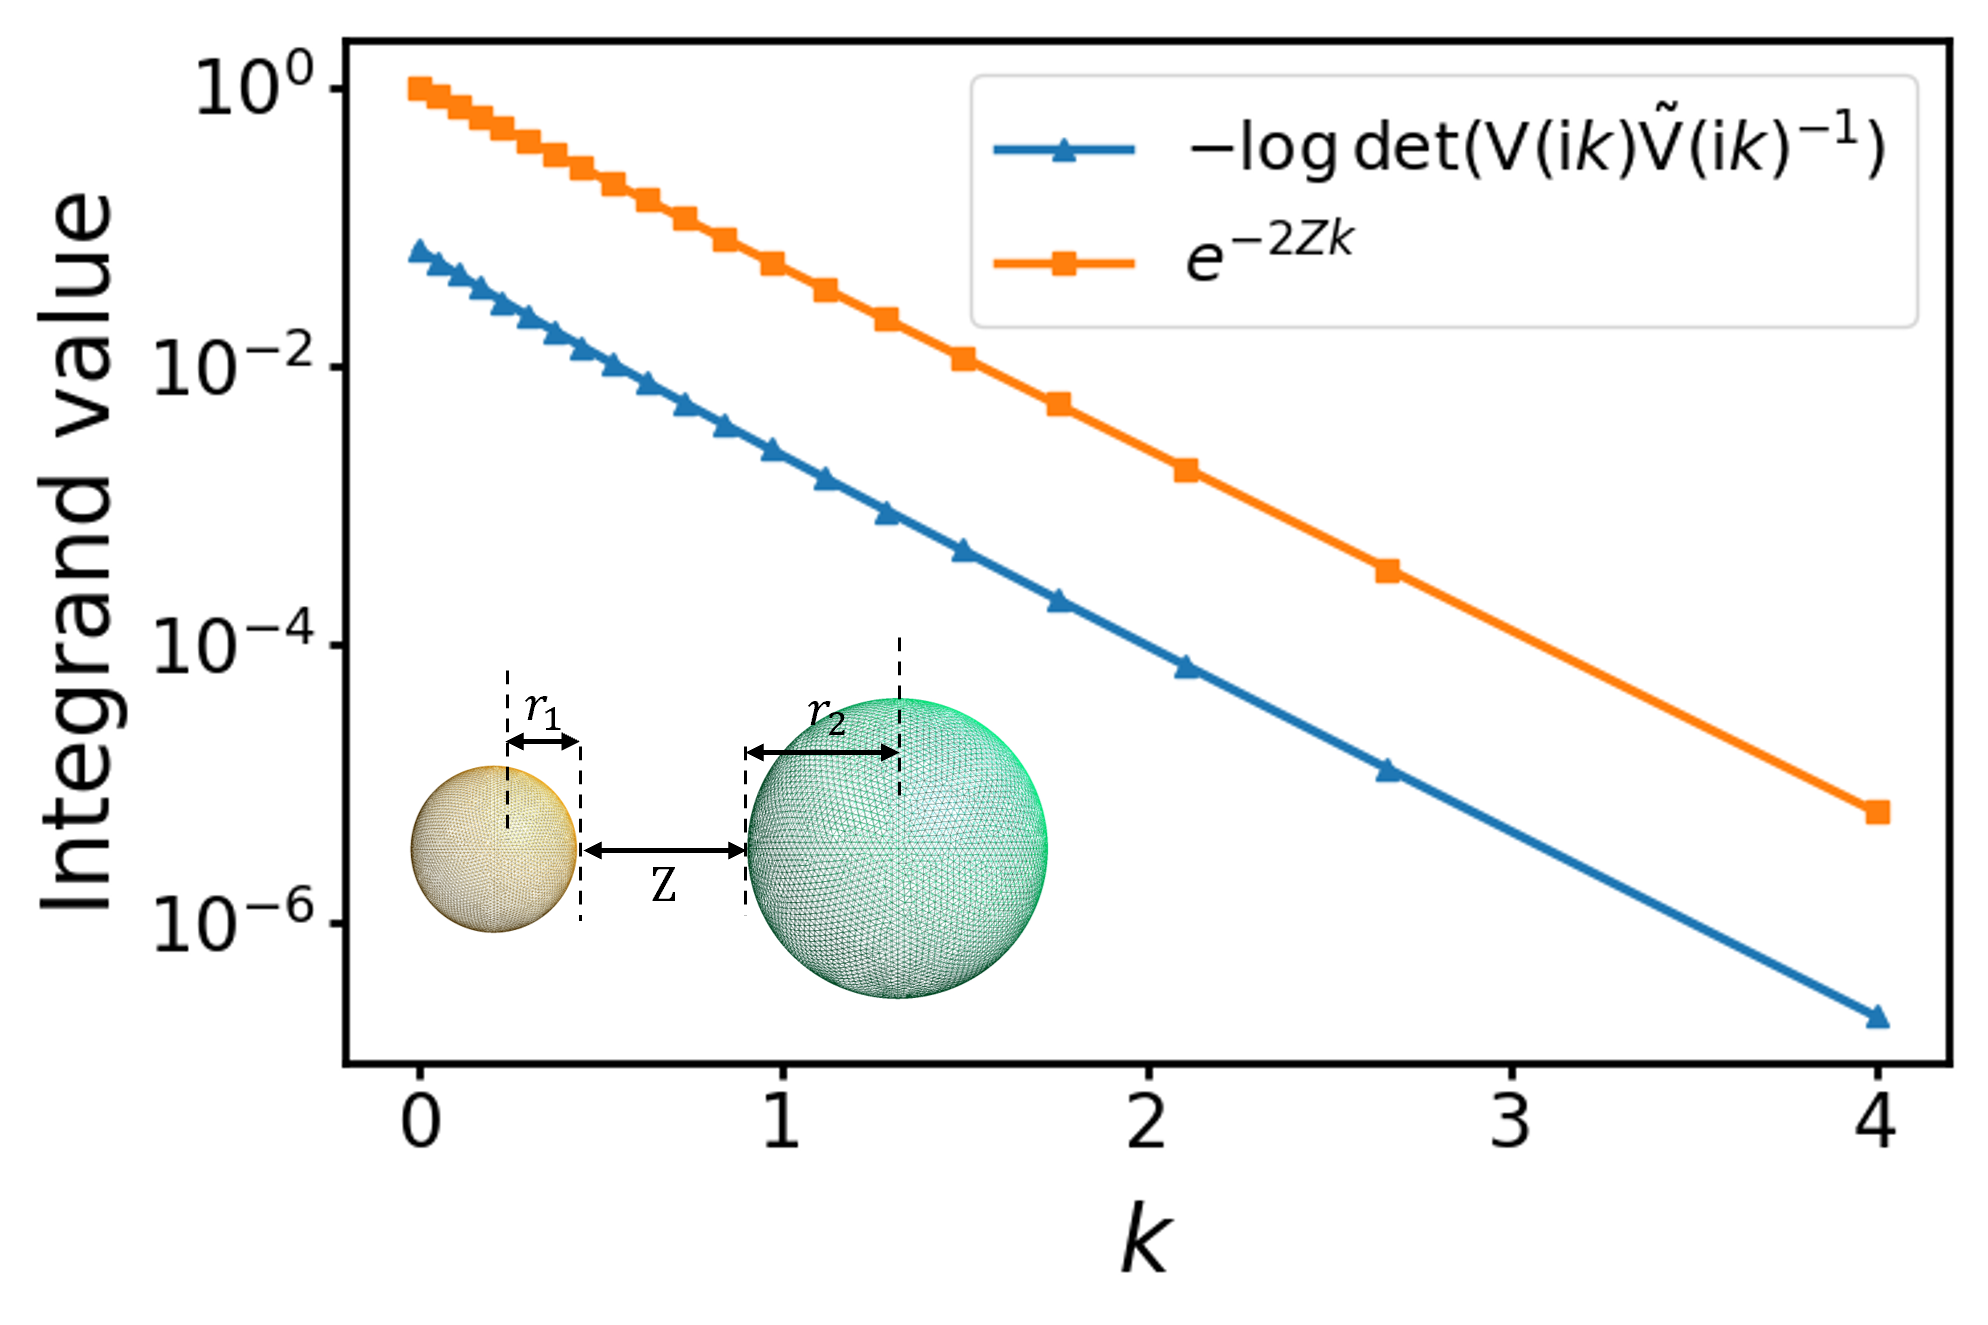
\includegraphics[scale = 0.7]{figures/Scalar_integ_decay_unequal.png}
    \caption{Exponential decay of $\Xi(\textrm{i}k)$ for two distinct spheres with radii $r_{1} = 0.5$ and $r_{2} = 1$ and minimum distance $Z=1.5$. The red line is the decay bound and the blue line is the actual decay.}
    \label{Distinct:The integrand decays exponentially}
\end{figure}

This purely linear algebraic consideration is not fully robust as it ignores the importance of the eigenvalue gap in the perturbation result. But we can 
heuristically explain the $\text{gap}$ as follows. On the continuous level the perturbations $E_1$ and $E_2$ are compact, so the tail end of the spectrum 
that converges to zero with small values of $\text{gap}_i$, is little affected by $E$, and the corresponding eigenvalues have a contribution of 
$\log \left|\frac{\lambda_i(A)}{\lambda_i(A+E)}\right| \approx 0$ to the value of $\Xi$. The relevant eigenvalues are the larger ones who for distinct obstacles 
have a sufficiently large value of $\text{gap}_i$.

While the linear algebra argument is useful to give a heuristical explanation, it is not as rigorous as the analytical result in \cite{fang2022trace}. In particular, we want to emphasize that the exponential decay bound with the quadratic factor also holds if the two obstacles are identical, which is not obvious from pure linear algebraic considerations. An example of this is given in Figure \ref{The integrand decays exponentially}.

\begin{figure}[H]
    \centering
    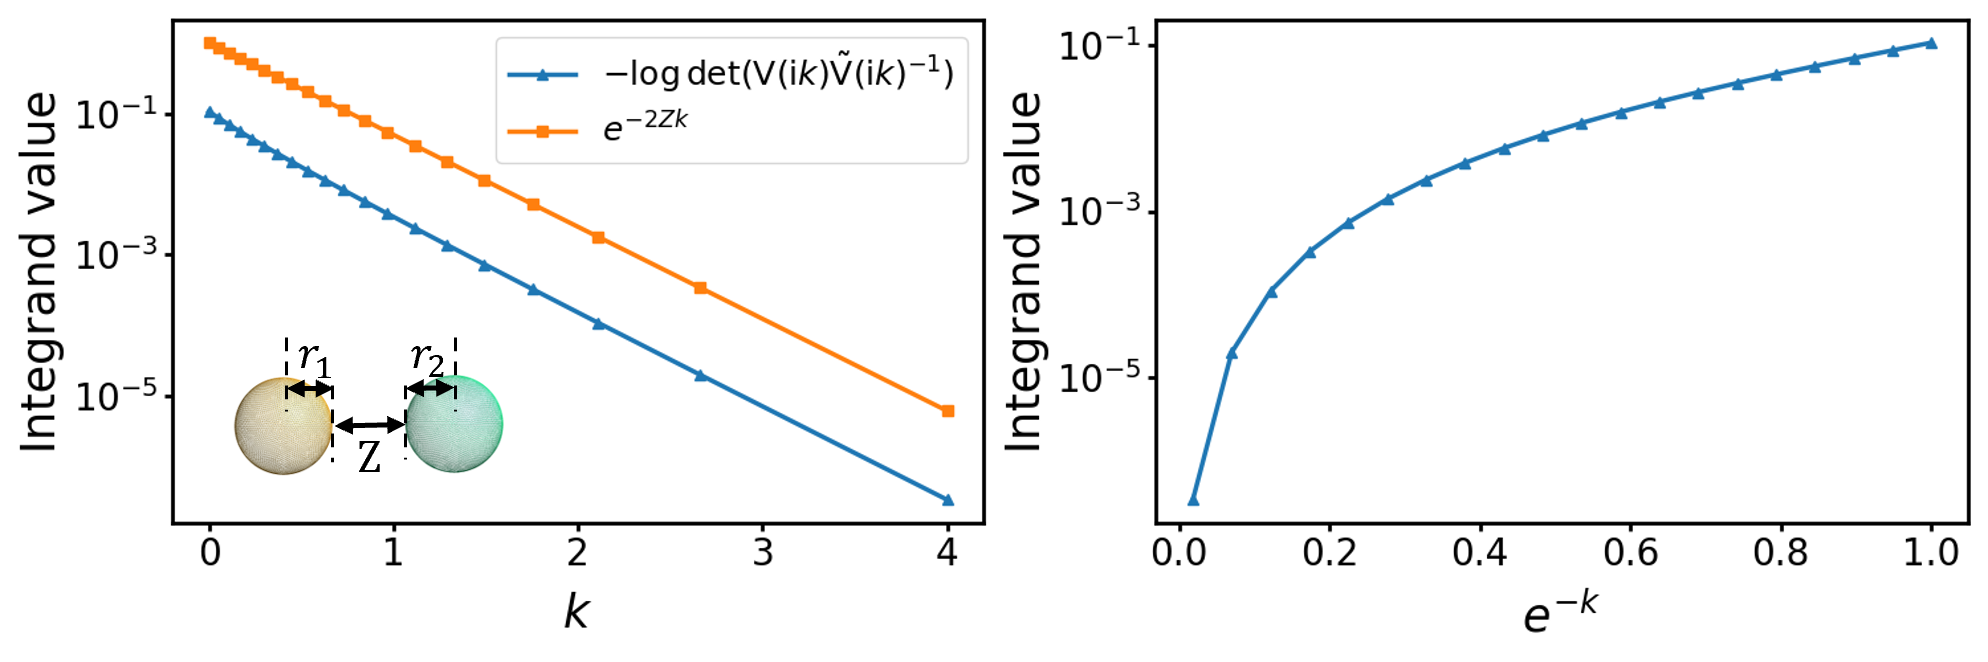
\includegraphics[width = \textwidth]{figures/Scalar_integ_decay.png}
    \caption{(Left) Exponential decay of $\Xi(\textrm{i}k)$ for two identical spheres with radius $r_1 = r_2 =1$ and minimum distance $Z=1.5$. The red line is the decay bound and the blue line is the actual decay. (Right) The integrand $\Xi(ik)$ after varlable transformation to apply a numerical trapezoid rule for its evaluation.}
    \label{The integrand decays exponentially}
\end{figure}

The exponentially decay property motivates a simple change of variables through $y = e^{-k}$ in the integrant $\Xi(\mathrm{i}k) = \log\det(\mathsf{V}(\mathrm{i}k)\tilde{\mathsf{V}}(\mathrm{i}k)^{-1})$, 
which after transformation we can numerically evaluate with a simple trapezoidal rule. Figure \ref{The integrand decays exponentially} (Right) plots the integrand with regard to the new variable $y$.


\section{Spectral property of the integral operators}\label{Spectral property of the integral operators}
{\color {blue} The matrix $M_{\infty}$ is a compact perturbation of matrix $M$, which makes the eigenvalues of them close to each other. Therefore, if we plot the eigenvalues of 
the matrix $MM_{\infty}^{-1}$, we can notice that there are many eigenvalues closed to 1 and nearly contributes nothing to the log determinant. This spectral property
inspires us to use some iteration method to approximate the extreme eigenvalues of $MM_{\infty}^{-1}$. In order to make the computation process more efficiently, 
we will introduce an inverse-free method to speed up this process which makes us deal with the large-scale problem in the future.}

\section{Inverse-free methods for computing $\log\det(\mathsf{V}_{\mathrm{i}k}\tilde{\mathsf{V}}_{\mathrm{i}k}^{-1})$}\label{Krylov subspace for generalized eigenvalue problem}
By Section \ref{Numerical methods for computing the Casimir energy}, to compute the Casimir energy, it is necessary to evaluate the term
$\log\frac{\det\mathsf{V}_{\mathrm{i}k}}{\det\tilde{\mathsf{V}}_{\mathrm{i}k}} = \log\det(\mathsf{V}_{\mathrm{i}k}\tilde{\mathsf{V}}_{\mathrm{i}k}^{-1})$ 
with different values of $k$. In this section, several efficient methods will be introduced to compute this log determinant.

The log determinant of the matrix $\mathsf{V}_{\mathrm{i}k}\tilde{\mathsf{V}}_{\mathrm{i}k}^{-1}$ is equal to the sum of the logarithm of the eigenvalues of 
$\mathsf{V}_{\mathrm{i}k}\tilde{\mathsf{V}}_{\mathrm{i}k}^{-1}$. Since $\tilde{\mathsf{V}}_{\mathrm{i}k}$ is a compact perturbation of $\mathsf{V}_{\mathrm{i}k}$,
most of the eigenvalues of the matrix $\mathsf{V}_{\mathrm{i}k}\tilde{\mathsf{V}}_{\mathrm{i}k}^{-1}$ are close to 1 
(shown in the Figure \ref{eigenvalues of VVtilde}) and contribute little on the value of Casimir energy.
Therefore, the computation process for the large-scale problem can become efficient if only multiple extreme eigenvalues 
that mainly contribute to the log determinant are computed. In addition, we should also avoid directly computing the inverse of the matrix $\tilde{\mathsf{V}}_{\mathrm{i}k}$
since the computational complexity is cubic with respect to the matrix dimension.

In what follows, one method called inverse-free Krylov subspace method will be introduced to computed multiple extreme eigenvalues. For each quadrature point
$k_{j}$, $j = 1, \dots, N$, one can directly apply this method to find the log determinant of 
$\mathsf{V}_{\mathrm{i}k_{j}}\tilde{\mathsf{V}}_{\mathrm{i}k_{j}}^{-1}$. However, by recalling Figure 
\ref{The integrand decays exponentially}, most of the quadrature points are closed to each other, which inspires us to recycle the subspace obtained from 
$\mathsf{V}_{\mathrm{i}k_{j}}\tilde{\mathsf{V}}_{\mathrm{i}k_{j}}^{-1}$ and use it for $\mathsf{V}_{\mathrm{i}k_{j+1}}\tilde{\mathsf{V}}_{\mathrm{i}k_{j+1}}^{-1}$'s case.
Afterwards, another efficient method based on LU decomposition for inverting the diagonal block matrix of $\tilde{\mathsf{V}}_{\mathrm{i}k}$ and applying
standard Arnoldi iterations will be demonstrated and its corresponding recycling-subspace-based method will be discussed as well.
Finally, the comparison of among these methods on their performance for approximating the log determinant and the number of matrix-vector multiplications 
will be shown.
\begin{figure}[H]
    \centering
    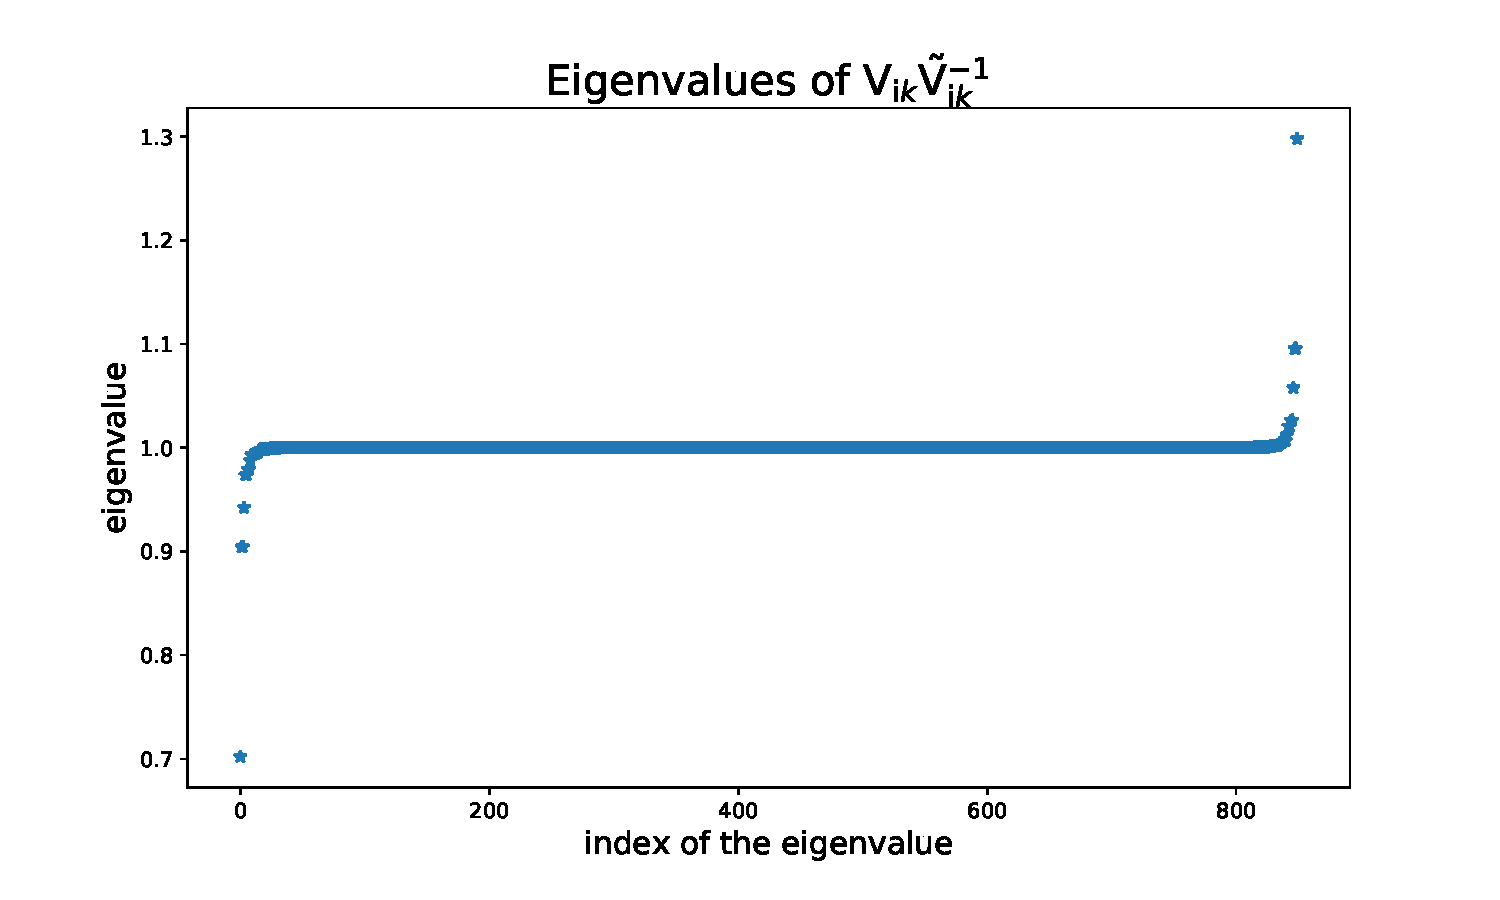
\includegraphics[scale = 0.5]{figures/eigenvalue_of_VVtilde.pdf}
    \caption{The eigenvalues of the matrix $\mathsf{V}_{\mathrm{i}k}\tilde{\mathsf{V}}_{\mathrm{i}k}^{-1}$ when $\mathrm{i}k = 0.8\mathrm{i}$.
    The scatterers are two spheres with equal radii $r_{1} = r_{2} = 1$ and the minimal distance between them is $Z = 0.5$. The grid size of the mesh is $h = 0.1$.}
    \label{eigenvalues of VVtilde}
\end{figure}
\subsection{Method I: Inverse-free Krylov subspace method}
Consider the eigenvalue problem: 
\begin{align} \label{EP}
    \mathsf{V}_{\mathrm{i}k}\tilde{\mathsf{V}}_{\mathrm{i}k}^{-1}\boldsymbol{x} = \lambda\boldsymbol{x},
\end{align}
where $\lambda$ is the eigenvalue and $\boldsymbol{x}$ is the corresponding eigenvalue. This eigenvalue problem is equivalent to the following generalized eigenvalue problem:
\begin{align}\label{GEP}
    \mathsf{V}_{\mathrm{i}k}\tilde{\boldsymbol{x}} = \lambda \tilde{\mathsf{V}}_{\mathrm{i}k}\tilde{\boldsymbol{x}}.
\end{align}
Thus, we can focus on solving the problem \eqref{GEP} instead of \eqref{EP} to avoid computing the matrix inversion. By \cite{golub2002inverse}\cite{money2005algorithm},
the authors proposed an inverse-free Krylov subspace method for computing a few extreme eigenvalues of the symmetric definite generalized eigenvalue problem 
and the following algorithm summarizes this method.

\begin{algorithm}[H]
    \SetAlgoLined
    Input: Symmetric matrix $A\in\mathbb{R}^{n\times n}$, s.p.d matrix $B\in\mathbb{R}^{n\times n}$, an initial approximation $\boldsymbol{x}$ with $||\boldsymbol{x}|| = 1$,
    the shift $\rho = 1$ and the dimension of the Krylov subspace $m\geq 1$\\
    Output: The approximated extreme eigenvalues of $A\boldsymbol{x} = \lambda B\boldsymbol{x}$\\
    \begin{algorithmic}[1]
        
        \STATE Construct a basis $Z_{m}$ for the Krylov subspace $K_{m} = \text{span}(\boldsymbol{x}, (A - \rho B)\boldsymbol{x}, \dots, (A - \rho B)^{m-1}\boldsymbol{x})$ with dimension $m$
        \STATE Project $A$ and $B$ on $Z$: $A_{m} = Z_{m}^{T}(A - \rho B)Z_{m}$, $B_{m} = Z_{m}^{T}BZ_{m}$
        \STATE Compute all the eigenpairs $\{(\lambda_{i}, \boldsymbol{x}_{i})\}_{i = 1, \dots, m}$ for the matrix pencil $(A_{m}, B_{m})$
        \STATE Add each eigenvalue in $\{\lambda_{i}\}_{i = 1, \dots, m}$ with the shift $\rho = 1$: $\tilde{\lambda}_{i} = \lambda_{i} + 1$, for $i = 1, \dots, m$
        \end{algorithmic}
    \caption{Inverse-free Krylov subspace method for computing multiple extreme eigenvalues of the generalized eigenvalue problem $A\boldsymbol{x} = \lambda B\boldsymbol{x}$}
    \label{Alg for computing the evals kry}
    \end{algorithm}
    
Algorithm \ref{Alg for computing the evals kry} can make us approximate $m$ extreme eigenvalues for the matrix pencil $(A,B)$ where $m$ is the dimension of the 
Krylov subspace $K_{m}$ in Step 1, Algorithm \ref{Alg for computing the evals kry}. Moreover, since most of the eigenvalues of $\mathsf{V}_{\mathrm{i}k}\tilde{\mathsf{V}}_{\mathrm{i}k}^{-1}$ are around 1,
it is better to set the shift $\rho$ as 1, otherwise, we need more iterations to make the eigenvalues approximate to the exact ones \cite{golub2002inverse}.

Therefore, for each quadrature point $\mathrm{i}k_{j}$, for $j = 1, \dots, N$, we can apply Algorithm \ref{Alg for computing the evals kry} to compute 
the eigenvalues $\{\lambda_{i}^{(j)}\}_{i = 1, \dots, m}$ for $\mathsf{V}_{\mathrm{i}k_{j}}\tilde{\mathsf{V}}_{\mathrm{i}k_{j}}^{-1}$, then the value of 
$\log\det(\mathsf{V}_{\mathrm{i}k_{j}}\tilde{\mathsf{V}}_{\mathrm{i}k_{j}}^{-1})$ can be approximated by 
\begin{align*}
    \log\det(\mathsf{V}_{\mathrm{i}k_{j}}\tilde{\mathsf{V}}_{\mathrm{i}k_{j}}^{-1}) \approx \sum_{i = 1}^{m} \log\left(\lambda_{i}^{(j)}\right), \ \ \ \ j = 1, \dots, N.
\end{align*}

In order to make this inverse-free method become more efficient, one can recycle the subspace obtained from the first wavenumber $\mathrm{i}k_{1}$ case by 
extracting several eigenvectors associated with the extremal eigenvalues in Step 3, Algorithm \ref{Alg for computing the evals kry} and recovering the 
eigenvectors for the matrix pair $(\mathsf{V}_{\mathrm{i}k_{1}}, \tilde{\mathsf{V}}_{\mathrm{i}k_{1}})$ by multiplying the basis $Z_{m}$ in Step 1, 
Algorithm \ref{Alg for computing the evals kry} with the extracted eigenvectors. After orthogonalizing the resulting vectors, they are recycled as a temporary basis
for the next wavenumber's case. 

For the second wavenumber, we initially compute the approximated eigenvalues ($\{\tilde{\lambda}_{i}\}$) and eigenvectors $\left(\{\tilde{\boldsymbol{x}}_{i}\}\right)$ with the 
recycled subspace and use the residual vectors $\left(\{\boldsymbol{r}_{i}\},\ \text{where}\ \boldsymbol{r}_{i} = \mathsf{V}_{\mathrm{i}k_{2}}\tilde{\boldsymbol{x}}_{2} - \tilde{\lambda}_{i}\tilde{\mathsf{V}}_{\mathrm{i}k_{1}}\tilde{\boldsymbol{x}}_{i}\right)$
to expand the temporary basis. With the expanded subspace, we recompute the eigenpairs for the second wavenumber's case and extract the resulting eigenvectors for the 
third wavenumber and so on. This modified inverse-free Krylov subspace method based on the recycled subspace is completely described in 
Algorithm \ref{Alg for computing the evals kry recycled}.

\begin{algorithm}[H]
    \SetAlgoLined
    Input: $N$: the number of matrix pencils ($A^{(i)}, B^{(i)}$), an initial approximation $\boldsymbol{x}$ with $||\boldsymbol{x}|| = 1$, the shift $\rho = 1$, the dimension of Krylov subspace $m\geq 1$ and the number of chosen extreme eigenvalues $\{s_{i}\}_{i}$, for $i = 1, 2, \dots, (N-1)$\\
    Output: The approximated extreme eigenvalues of $A\boldsymbol{x} = \lambda B\boldsymbol{x}$\\

    \begin{algorithmic}[1]
        \STATE When $i = 1$:
        \begin{itemize}
            \item[(a)] Compute the basis $Z_{m}^{(1)}$ for the Krylov subspace $K_{m}^{(1)} = \text{span}\left(\boldsymbol{x}, (A^{(1)} - \rho B^{(1)})\boldsymbol{x}, \dots, (A^{(1)} - \rho B^{(1)})^{m-1}\boldsymbol{x}\right)$ with dimension $m$
            
            \item[(b)] Project $A^{(1)}$ and $B^{(1)}$ on $Z_{m}^{(1)}$: 
            $A_{m}^{(1)} = Z_{m}^{(1)H}(A^{(1)} - \rho B^{(1)})Z_{m}^{(1)},\  B_{m}^{(1)} = Z_{m}^{(1)H}B^{(1)}Z_{m}^{(1)}$

    
            \item[(c)] Compute the eigenvalues $\boldsymbol{\lambda}^{(1)} = \{\lambda_{1}^{(1)}, \dots, \lambda_{m}^{(1)}\}$ and eigenvectors $\boldsymbol{X}_{m}^{(1)} = \left[\boldsymbol{x}_{1}^{(1)}, \dots, \boldsymbol{x}_{m}^{(1)}\right]$ for $A_{m}^{(1)}\boldsymbol{x} = \lambda B_{m}^{(1)}\boldsymbol{x}$ and note that the approximated eigenvalues for $A^{(1)}\boldsymbol{x} = \lambda B^{(1)}\boldsymbol{x}$ are $\{\lambda_{1}^{(1)}+\rho, \dots, \lambda_{m}^{(1)}+\rho\}$
            
            \item[(d)] Extract $s_{1}$ eigenvectors from $\boldsymbol{X}_{m}^{(1)}$, which correspond to $s_{1}$ extreme eigenvalues and relabel them as $\boldsymbol{X}_{s_{1}}^{(1)} = \left[\boldsymbol{x}_{1}^{(1)}, \dots, \boldsymbol{x}_{s_{1}}^{(1)}\right]$
            
            \item[(e)] Recover the eigenvectors for$A^{(1)}\boldsymbol{x} = \lambda B^{(1)}\boldsymbol{x}$ by computing $Z_{m}^{(1)}\boldsymbol{X}_{s_{1}}^{(1)}$ and orthogonalize it to obtain the temporary basis $\tilde{Z}_{s_{1}}^{(2)} = \text{orth}\left(Z_{m}^{(1)}\boldsymbol{X}_{s_{1}}^{(1)}\right)$ for the second matrix pencil ($A^{(2)}, B^{(2)}$)
        \end{itemize}
        
        \STATE When $i = 2$:
        \begin{itemize}
            \item[(a)] Project $A^{(2)}$ and $B^{(2)}$ on $\tilde{Z}_{s_{1}}^{(2)}$: 
            $\tilde{A}_{s_{1}}^{(2)} = \tilde{Z}_{s_{1}}^{(2)H}A^{(2)} \tilde{Z}_{s_{1}}^{(2)},  \tilde{B}_{s_{1}}^{(2)} = \tilde{Z}_{s_{1}}^{(2)H}B^{(2)}\tilde{Z}_{s_{1}}^{(2)}$

            \item[(b)] Compute the eigenvalues $\tilde{\boldsymbol{\lambda}}^{(2)} = \{\tilde{\lambda}_{1}^{(2)}, \dots, \tilde{\lambda}_{s_{1}}^{(2)}\}$ and eigenvectors $\tilde{\boldsymbol{X}}_{s_{1}}^{(2)} = \left[\tilde{\boldsymbol{x}}_{1}^{(2)}, \dots, \tilde{\boldsymbol{x}}_{s_{1}}^{(2)}\right]$ for $\tilde{A}_{s_{1}}^{(2)}\boldsymbol{x} = \lambda \tilde{B}_{s_{1}}^{(1)}\boldsymbol{x}$
            
            \item[(c)] Compute the residuals $\boldsymbol{r}_{i}^{(2)} = A^{(2)}\tilde{Z}_{s_{1}}^{(2)}\tilde{\boldsymbol{x}}_{i}^{(2)} - \tilde{\lambda}_{i}^{(2)}B^{(2)}\tilde{Z}_{s_{1}}^{(2)}\tilde{\boldsymbol{x}}_{i}^{(2)}$ for $i = 1, 2, \dots, s_{1}$ and denote $\boldsymbol{r}^{(2)} = \left[\boldsymbol{r}_{1}^{(2)}, \dots, \boldsymbol{r}_{s_{1}}^{(2)}\right]$
            
            \item[(d)] Construct the basis $Z_{2s_{1}}^{(2)}$ for $(A^{(2)}, B^{(2)})$ by extending the temporary basis $\tilde{Z}_{s_{1}}^{(2)}$ with the residues $\boldsymbol{r}^{(2)}$ and orthogonalizing the extended subspace: $Z_{2s_{1}}^{(2)} = \left[\tilde{Z}_{s_{1}}^{(2)}, \tilde{\boldsymbol{r}}^{(2)}\right]$, where $\tilde{\boldsymbol{r}}^{(2)} = \text{orth}\left(\boldsymbol{r}^{(2)}\right)$
            
            \item[(e)] Project $A^{(2)}$ and $B^{(2)}$ on $Z_{2s_{1}}^{(2)}$: 
            \begin{align*}
                A_{2s_{1}}^{(2)} &= Z_{2s_{1}}^{(2)H}A^{(2)} Z_{2s_{1}}^{(2)} = \begin{bmatrix}
                 \tilde{A}_{s_{1}}^{(2)} & \tilde{Z}_{s_{1}}^{(2)H}A^{(2)} \tilde{\boldsymbol{r}}^{(2)}\\
                 \tilde{\boldsymbol{r}}^{(2)H} A^{(2)} \tilde{Z}_{s_{1}}^{(2)} & \tilde{\boldsymbol{r}}^{(2)H} A^{(2)} \tilde{\boldsymbol{r}}^{(2)}
                \end{bmatrix}, \\
                B_{2s_{1}}^{(2)} &= Z_{2s_{1}}^{(2)H}B^{(2)}Z_{2s_{1}}^{(2)} = \begin{bmatrix}
                 \tilde{B}_{s_{1}}^{(2)} & \tilde{Z}_{s_{1}}^{(2)H}B^{(2)} \tilde{\boldsymbol{r}}^{(2)}\\
                 \tilde{\boldsymbol{r}}^{(2)H} B^{(2)} \tilde{Z}_{s_{1}}^{(2)} & \tilde{\boldsymbol{r}}^{(2)H} B^{(2)} \tilde{\boldsymbol{r}}^{(2)}
                \end{bmatrix}
            \end{align*}
            \item[(f)] Repeat Step 1(c)-(e) for these projected matrices to compute the approximated eigenvalues $\boldsymbol{\lambda}^{(2)} = \{\lambda_{1}^{(2)}, \dots, \lambda_{2s_{1}}^{(2)}\}$  and eigenvectors $\boldsymbol{X}_{2s_{1}}^{(2)} = \left[\boldsymbol{x}_{1}^{(2)}, \dots, \boldsymbol{x}_{2s_{1}}^{(2)}\right]$ for $\left( A_{2s_{1}}^{(2)},  B_{2s_{1}}^{(2)}\right)$ and obtain the temporary basis $\tilde{Z}_{s_{2}}^{(3)}$ for the third matrix pencil $\left(A^{(3)}, B^{(3)}\right)$
        \end{itemize}
        
        \STATE For $i = 3, \dots, N$, repeat the Step 2 to compute the approximated eigenvalues $\boldsymbol{\lambda}^{(i)} = \{\lambda_{1}^{(i)}, \dots, \lambda_{2s_{i-1}}^{(i)}\}$  and eigenvectors $\boldsymbol{X}_{2s_{i-1}}^{(i)} = \left[\boldsymbol{x}_{1}^{(i)}, \dots, \boldsymbol{x}_{2s_{i-1}}^{(i)}\right]$ for each matrix pencil
        \end{algorithmic}
    \caption{Inverse-free recycled Krylov subspace method for sequences of generalized eigenvalue problems $A^{(i)}\boldsymbol{x} = \lambda B^{(i)}\boldsymbol{x}$}
    \label{Alg for computing the evals kry recycled}
    \end{algorithm}    

In this case, the value of 
$\log\det(\mathsf{V}_{\mathrm{i}k_{j}}\tilde{\mathsf{V}}_{\mathrm{i}k_{j}}^{-1})$ can be approximated by 
\begin{equation}
    \log\det(\mathsf{V}_{\mathrm{i}k_{j}}\tilde{\mathsf{V}}_{\mathrm{i}k_{j}}^{-1})  \approx
      \begin{cases}
        \sum_{i = 1}^{m} \log\left(\lambda_{i}^{(j)}\right) & j = 1\\
        \sum_{i = 1}^{2s_{j-1}} \log\left(\lambda_{i}^{(j)}\right) & j = 2, \dots, N
      \end{cases}       
  \end{equation}

\subsection{Method II: Standard Arnoldi method}
Another efficient approach for computing $\log\det(\mathsf{V}_{\mathrm{i}k}\tilde{\mathsf{V}}_{\mathrm{i}k}^{-1})$ is to initially construct the Krylov subspace  
$K_{m}(\mathsf{V}_{\mathrm{i}k}\tilde{\mathsf{V}}_{\mathrm{i}k}^{-1}, \boldsymbol{b})$, where $\boldsymbol{b}$ is some 
initial vector and $m$ is the dimension of this Krylov subspace. Afterwards, we implement the standard Arnoldi iteration to obtain the orthogonal basis of 
this order-$m$ Krylov subspace and project the matrix $\mathsf{V}_{\mathrm{i}k}\tilde{\mathsf{V}}_{\mathrm{i}k}^{-1}$ onto this basis. 
This projection matrix is called the Hessenberg matrix and we denote it as $H_{m}$. By \cite{saad2011numerical}, the eigenvalues of $H_{m}$ (which are also 
called Ritz eigenvalues) can give good approximations on extreme eigenvalues of $\mathsf{V}_{\mathrm{i}k}\tilde{\mathsf{V}}_{\mathrm{i}k}^{-1}$.
The following algorithm lists the general steps described above.


\begin{algorithm}[H]
    \SetAlgoLined
    Input: Block matrix $A\in\mathbb{R}^{n\times n}$, diagonal block matrix $B\in\mathbb{R}^{n\times n}$ and the dimension of the Krylov subspace $m\geq 1$\\
    Output: The approximated extreme eigenvalue of $AB^{-1}\boldsymbol{x} = \mu \boldsymbol{x}$\\
    \begin{algorithmic}[1]
        \STATE Use standard Arnoldi method to compute the Hessenberg matrix $H_{m}$ of $AB^{-1}$
        \STATE Compute all the eigenpairs $\{(\mu_{i}, \boldsymbol{x}_{i})\}_{i = 1, \dots, m}$ of $H_{m}$
        \end{algorithmic}
    \caption{Standard Arnoldi method for computing multiple extreme eigenvalues of the eigenvalue problem $AB^{-1}\boldsymbol{x} = \mu\boldsymbol{x}$}
    \label{Alg for arno method}
    \end{algorithm}

\begin{remark}
    During the Arnoldi iteration process, one needs to multiply the inverse matrix $\tilde{\mathsf{V}}_{\mathrm{i}k}^{-1}$ with some vector 
$\boldsymbol{v} = \begin{bmatrix}\boldsymbol{v}_{1}\\ \vdots \\ \boldsymbol{v}_{N} \end{bmatrix}$. In order to avoid directly computing 
the matrix inversion, one can firstly compute LU decomposition for each diagonal 
block matrix $\mathsf{V}_{ii}(\mathrm{i}k) = \mathsf{L}_{ii}\mathsf{U}_{ii} $, for $i = 1, 2, \dots, N$, where $\mathsf{L}_{ii}$ and $\mathsf{U}_{ii}$ are lower and upper triangular matrices, 
respectively and solve the linear system $\mathsf{L}_{ii}\mathsf{U}_{ii}\boldsymbol{x}_{i} = \boldsymbol{v}_{i}$ for $i = 1, 2, \dots, N$. Finally, the resulting 
vector is $\boldsymbol{x} = \begin{bmatrix}\boldsymbol{x}_{1}\\ \vdots \\ \boldsymbol{x}_{1} \end{bmatrix}$.
\end{remark}


By denoting the the eigenvalues of $H_{m}$ as $\{\mu_{i}\}_{i = 1, \dots, m}$, the value of  
$\log\det(\mathsf{V}_{\mathrm{i}k}\tilde{\mathsf{V}}_{\mathrm{i}k}^{-1})$ can be approximated by
\begin{align*}
    \log\det(\mathsf{V}_{\mathrm{i}k}\tilde{\mathsf{V}}_{\mathrm{i}k}^{-1}) \approx \sum_{i = 1}^{m}\log\left(\mu_{i}\right).
\end{align*}

Same with the inverse-free Krylov subspace method, one can also recycle the eigenvectors associated with the extreme eigenvalues from the initial subspace 
for the first wavenumber, expand it with some vectos (In Algorithm \ref{Alg for computing the evals kry recycled}, they are residual vectors) and 
use the complemented basis for the second wavenumber's case. Algorithm \ref{Alg for computing the evals arno recycled} summarizes the whole steps for this 
recycling process. 

\begin{algorithm}[H]
    \SetAlgoLined
    Input: $N$: the number of matrices $A^{(i)}\left(B^{(i)}\right)^{-1}$, where $A^{(i)}$ are block matrices and $B^{(i)}$ are diagonal block matrices, an initial approximation $\boldsymbol{x}$ with $||\boldsymbol{x}|| = 1$, the shift $\rho = 1$, the dimension of Krylov subspace $m\geq 1$ and the number of chosen extreme eigenvalues $\{s_{i}\}_{i}$, for $i = 1, 2, \dots, (N-1)$\\
    \vspace{0.5cm}
    \begin{algorithmic}[1]
        \STATE When $i = 1$:
        \begin{itemize}
            
            \item[(a)]Apply the standard Arnoldi method to compute the Arnoldi vectors $Z_{m}^{(1)}$ and Hessenberg matrix $H_{m}^{(1)}$ for $A^{(1)}\left(B^{(1)}\right)^{-1}$, which satisfies $H_{m}^{(1)} = Z_{m}^{(1)H}\left(A^{(1)}\left(B^{(1)}\right)^{-1}\right)Z_{m}^{(1)}$
    
            \item[(b)] Compute the eigenvalues $\boldsymbol{\mu}^{(1)} = \{\mu_{1}^{(1)}, \dots, \mu_{m}^{(1)}\}$ and eigenvectors $\boldsymbol{X}_{m}^{(1)} = \left[\boldsymbol{x}_{1}^{(1)}, \dots, \boldsymbol{r}_{m}^{(1)}\right]$ for $H_{m}^{(1)}$
            
            \item[(c)] Extract $s_{1}$ eigenvectors from $\boldsymbol{X}_{m}^{(1)}$, which correspond to $s_{1}$ extreme eigenvalues and relabel them as $\boldsymbol{X}_{s_{1}}^{(1)} = \left[\boldsymbol{x}_{1}^{(1)}, \dots, \boldsymbol{x}_{s_{1}}^{(1)}\right]$
            
            \item[(d)] Recover the eigenvectors for $A^{(1)}\left(B^{(1)}\right)^{-1}x = \mu x$ by computing $Z_{m}^{(1)}\boldsymbol{X}_{s_{1}}^{(1)}$ and orthogonalize it to obtain the temporary basis $\tilde{Z}_{s_{1}}^{(2)} = \text{orth}\left(Z_{m}^{(1)}\boldsymbol{X}_{s_{1}}^{(1)}\right)$ for the second eigenvalue problem $A^{(2)}\left(B^{(2)}\right)^{-1}\boldsymbol{x} = \lambda \boldsymbol{x}$
        \end{itemize}
        
        \STATE When $i = 2$:
        \begin{itemize}
            \item[(a)] Project $A^{(2)}\left(B^{(2)}\right)^{-1}$ on $\tilde{Z}_{s_{1}}^{(2)}$: 
            \begin{align*}
                \tilde{H}_{s_{1}}^{(2)} &= \tilde{Z}_{s_{1}}^{(2)H}\left(A^{(2)}\left(B^{(2)}\right)^{-1}\right) \tilde{Z}_{s_{1}}^{(2)}
            \end{align*}
            
            \item[(b)] Compute the eigenvalues $\tilde{\boldsymbol{\mu}}^{(2)} = \{\tilde{\mu}_{1}^{(2)}, \dots, \tilde{\mu}_{s_{1}}^{(2)}\}$ and eigenvectors $\tilde{\boldsymbol{X}}_{s_{1}}^{(2)} = \left[\tilde{\boldsymbol{x}}_{1}^{(2)}, \dots, \tilde{\boldsymbol{x}}_{s_{1}}^{(2)}\right]$ for $A^{(2)}\left(B^{(2)}\right)^{-1}x = \lambda x$
            
            
            \item[(c)] Compute the residuals $\boldsymbol{r}_{i}^{(2)} = \left(A^{(2)}\left(B^{(2)}\right)^{-1}\right)\tilde{Z}_{s_{1}}^{(2)}\tilde{\boldsymbol{x}}_{i}^{(2)} - \tilde{\mu}_{i}^{(2)}\tilde{Z}_{s_{1}}^{(2)}\tilde{\boldsymbol{x}}_{i}^{(2)}$, for $i = 1, 2, \dots, s_{1}$ and denote $\boldsymbol{r}^{(2)} = \left[\boldsymbol{r}_{1}^{(2)}, \dots, \boldsymbol{r}_{s_{1}}^{(2)}\right]$
            
            \item[(d)] Construct the basis $Z_{2s_{1}}^{(2)}$ for $A^{(2)}\left(B^{(2)}\right)^{-1}$ by extending the temporary basis $\tilde{Z}_{s_{1}}^{(2)}$ with the residues $\boldsymbol{r}^{(2)}$ and orthogonalizing the extended subspace: $Z_{2s_{1}}^{(2)} = \left[\tilde{Z}_{s_{1}}^{(2)}, \tilde{\boldsymbol{r}}^{(2)}\right]$, where $\tilde{\boldsymbol{r}}^{(2)} = \text{orth}\left(\boldsymbol{r}^{(2)}\right)$
            
            \item[(e)] Project $A^{(2)}\left(B^{(2)}\right)^{-1}$ on $Z_{2s_{1}}^{(2)}$: 
            \begin{align*}
                H_{2s_{1}}^{(2)} = Z_{2s_{1}}^{(2)H}\left(A^{(2)}\left(B^{(2)}\right)^{-1}\right) Z_{2s_{1}}^{(2)} = \begin{bmatrix}
                 \tilde{H}_{s_{1}}^{(2)} & \tilde{Z}_{s_{1}}^{(2)H}\left(A^{(2)}\left(B^{(2)}\right)^{-1}\right) \tilde{\boldsymbol{r}}^{(2)}\\
                 \tilde{\boldsymbol{r}}^{(2)H}\left(A^{(2)}\left(B^{(2)}\right)^{-1}\right) \tilde{Z}_{s_{1}}^{(2)} & \tilde{\boldsymbol{r}}^{(2)H}\left(A^{(2)}\left(B^{(2)}\right)^{-1}\right) \tilde{\boldsymbol{r}}^{(2)}
                \end{bmatrix}
            \end{align*}
            \item[(f)] Repeat Step 1(c)-(e) for the projected matrix $ H_{2s_{1}}^{(2)}$ to compute the approximated eigenvalues $\boldsymbol{\mu}^{(2)} = \{\mu{1}^{(2)}, \dots, \mu{2s_{1}}^{(2)}\}$  and eigenvectors $\boldsymbol{X}_{2s_{1}}^{(2)} = \left[\boldsymbol{x}_{1}^{(2)}, \dots, \boldsymbol{x}_{2s_{1}}^{(2)}\right]$ and obtain the temporary basis $\tilde{Z}_{s_{2}}^{(3)}$ for the third eigenvalue problem $A^{(3)}\left(B^{(3)}\right)^{-1}x = \lambda x$
        \end{itemize}
        
        \STATE For $i = 3, \dots, N$, repeat the Step 2 to compute the approximated eigenvalues $\boldsymbol{\mu}^{(i)} = \{\mu_{1}^{(i)}, \dots, \mu_{2s_{i-1}}^{(i)}\}$  and eigenvectors $\boldsymbol{X}_{2s_{i-1}}^{(1)} = \left[\boldsymbol{x}_{1}^{(i)}, \dots, \boldsymbol{x}_{2s_{i-1}}^{(i)}\right]$ for each eigenvalue problem
        \end{algorithmic}
    \caption{Standard Arnoldi methods with recycled subspaces for sequences of  eigenvalue problems $A^{(i)}\left(B^{(i)}\right)^{-1} \boldsymbol{x} = \mu \boldsymbol{x}$}
    \label{Alg for computing the evals arno recycled}
    \end{algorithm}    
 
With Algorithm \ref{Alg for computing the evals arno recycled}, the value of 
$\log\det(\mathsf{V}_{\mathrm{i}k_{j}}\tilde{\mathsf{V}}_{\mathrm{i}k_{j}}^{-1})$ can be approximated by 


\begin{equation}
    \log\det(\mathsf{V}_{\mathrm{i}k_{j}}\tilde{\mathsf{V}}_{\mathrm{i}k_{j}}^{-1})  \approx
      \begin{cases}
        \sum_{i = 1}^{m} \log\left(\mu_{i}^{(j)}\right) & j = 1\\
        \sum_{i = 1}^{2s_{j-1}} \log\left(\mu_{i}^{(j)}\right) & j = 2, \dots, N
      \end{cases}       
  \end{equation}

\subsection{Comparison between inverse-free Krylov subspace and standard Arnoldi method with or without recycling subspaces}
In this part, the performances on approximating the $\log\det\mathsf{V}_{\mathrm{i}k}\tilde{\mathsf{V}}_{\mathrm{i}k}^{-1}$ and the complexity 
of Algorithm \ref{Alg for computing the evals kry}-\ref{Alg for computing the evals arno recycled} will be compared.
Consider two spheres with equal radii $r_{1} = r_{2} = 1$ and the minimal distance between them is denoted as $Z$, which is set as 0.5, 1.5 and 3.0. 
The dimension of the Krylov subspace $m$ in Algorithm \ref{Alg for computing the evals kry}, Algorithm \ref{Alg for computing the evals kry recycled}, Step 1 of Algorithm \ref{Alg for computing the evals kry recycled},
Algorithm \ref{Alg for arno method} and Step 1 of Algorithm \ref{Alg for computing the evals arno recycled} 
is $m = 100$. The rule for extracting the eigenvectors in recycled scheme is that only the eigenvector associated with the extreme eigenvalue whose 
logarithm value is greater than $10^{-5}$ would be recycled.

Table \ref{Table lists the logdet} lists the relative error for approximating the value of $\log\det\mathsf{V}_{\mathrm{i}k}\tilde{\mathsf{V}}_{\mathrm{i}k}^{-1}$ 
computed via the inverse-free Krylov subspace method and standard Arnoldi method with or without recycling the subspace. It indicates that for with the settings above, one 
can have at lease three significant digits accuracy.
 
\begin{table}[H]
    \centering
    \begin{tabular}{ |M{1.5cm}|M{1.7cm}|M{2.2cm} |M{2.2cm}|M{2.2cm}|M{3cm}|M{2.2cm}| } 
    \hline
    Distance $Z$ & Quadrature points $k$ &  Inverse-free (no recycling) & Inverse-free (recycling) & Standard Arnoldi (no recycling) & Standard Arnoldi (recycling)\\
    \hline
    \multirow{5}{4em}{$Z = 0.5$}   & 0        & $9.79\times 10^{-4}$  & $9.79\times 10^{-4}$  &$9.29\times 10^{-4}$ &$9.29\times 10^{-4}$\\ 
                                   & 0.0540   & $9.67\times 10^{-4}$  & $9.78\times 10^{-5}$  &$4.91\times 10^{-5}$ &$1.37\times 10^{-6}$\\ 
                                   & 0.111    & $1.22\times 10^{-3}$  & $2.79\times 10^{-5}$  &$5.29\times 10^{-5}$ &$5.17\times 10^{-6}$\\ 
                                   & 0.171    & $1.15\times 10^{-3}$  & $2.42\times 10^{-5}$  &$2.78\times 10^{-5}$ &$8.45\times 10^{-5}$\\ 
                                   & 0.236    & $1.25\times 10^{-3}$  & $9.10\times 10^{-6}$  &$1.12\times 10^{-4}$ &$2.76\times 10^{-5}$\\ 
    \hline
    \hline
    \multirow{5}{4em}{$Z = 1.5$}   & 0        & $9.48\times 10^{-4}$  & $9.54\times 10^{-4}$  &$3.41\times 10^{-7}$ &$3.41\times 10^{-7}$\\ 
                                   & 0.0540   & $1.02\times 10^{-3}$  & $2.87\times 10^{-4}$  &$5.89\times 10^{-7}$ &$3.97\times 10^{-8}$\\ 
                                   & 0.111    & $1.16\times 10^{-3}$  & $1.80\times 10^{-4}$  &$1.45\times 10^{-8}$ &$2.35\times 10^{-4}$\\ 
                                   & 0.171    & $1.25\times 10^{-3}$  & $1.35\times 10^{-4}$  &$2.70\times 10^{-6}$ &$1.06\times 10^{-4}$\\ 
                                   & 0.236    & $1.33\times 10^{-3}$  & $4.77\times 10^{-5}$  &$3.14\times 10^{-7}$ &$4.87\times 10^{-5}$\\ 
    \hline
    \hline
    \multirow{5}{4em}{$Z = 3.0$}   & 0        & $1.38\times 10^{-3}$  & $1.38\times 10^{-3}$  &$8.55\times 10^{-12}$ &$8.55\times 10^{-12}$\\ 
                                   & 0.0540   & $1.54\times 10^{-3}$  & $4.34\times 10^{-4}$  &$3.46\times 10^{-9}$  &$2.61\times 10^{-5}$\\ 
                                   & 0.111    & $1.81\times 10^{-3}$  & $2.89\times 10^{-4}$  &$5.02\times 10^{-10}$ &$5.43\times 10^{-7}$\\ 
                                   & 0.171    & $2.13\times 10^{-3}$  & $2.35\times 10^{-4}$  &$4.82\times 10^{-8}$  &$2.50\times 10^{-5}$\\ 
                                   & 0.236    & $2.54\times 10^{-3}$  & $2.13\times 10^{-4}$  &$5.07\times 10^{-9}$  &$1.59\times 10^{-5}$\\ 
    \hline
    \end{tabular}
    \caption{Relative error for approximating the value of $\log\det\mathsf{V}_{\mathrm{i}k}\tilde{\mathsf{V}}_{\mathrm{i}k}^{-1}$ on the first five consecutive 
    quadrature points via the inverse-free Krylov subspace and standard Arnoldi methods with/without subspace recycled. The scatterers are two spheres with 
    equal radii $R = 1$ with distance $Z = 0.5$, 1.5 and 3.0}
    \label{Table lists the logdet}
    \end{table}

To further compare the efficiency of these methods, we explore the number of matrix-vector multiplications for these methods on computing the Casimir energy
and they are list inside Table \ref{4methods FLOP}. In addition, Figure \ref{matvec100} and Figure \ref{matvec200} plot the number of matrix-vector multiplications
that we need to compute the Casimir energy between two spheres with distance $Z = 0.5$, 1.5 and 3.0 by using these methods with or without recycling the subspaces.
One can notice that the methods with recycling the subspace  have similar number of matvec and they also have smaller number of matvec than the non-recycling methods.
Therefore, for all the numerical experiments in Section \ref{Numerical experiments}, we would apply the methods with subspaced recycled to compute the Casimir energy.
\begin{table}[H]
    \centering
\begin{tabular}{ |P{4cm}|P{4cm}|P{4cm}|P{4cm}|  }
    \hline
    \multicolumn{2}{|c|}{Inverse-free Krylov subspace method}& \multicolumn{2}{c|}{Standard Arnoldi method} \\
    \hline
   Without recycling &  With recycling & Without recycling& With recycling\\
    \hline
    $(2m - 1)N$  & $(2m - 1) + 2\sum_{i = 1}^{N-1}s_{i}$   & $(m - 1)N$ &   $(m - 1) + 2\sum_{i = 1}^{N-1}s_{i}$ \\
    \hline
   \end{tabular}
   \caption{The number of matrix-vector multiplications inside the inverse-free Krylov subspace and standard Arnoldi methods with or without recycling subspaces.
   $N$ is the number of wavenumbers, $m$ is the dimension of the Krylov subspace for the first wavenumber (in recycling case); for all the wavenumbers (in non-recycling case),
   and $s_{i}$ is the number of the extracted eigenvectors 
   for the $i$th wavenumber's case (in recycling case).}
   \label{4methods FLOP}
\end{table}
\begin{figure}[H]
    \centering
    \hspace*{-1.5cm}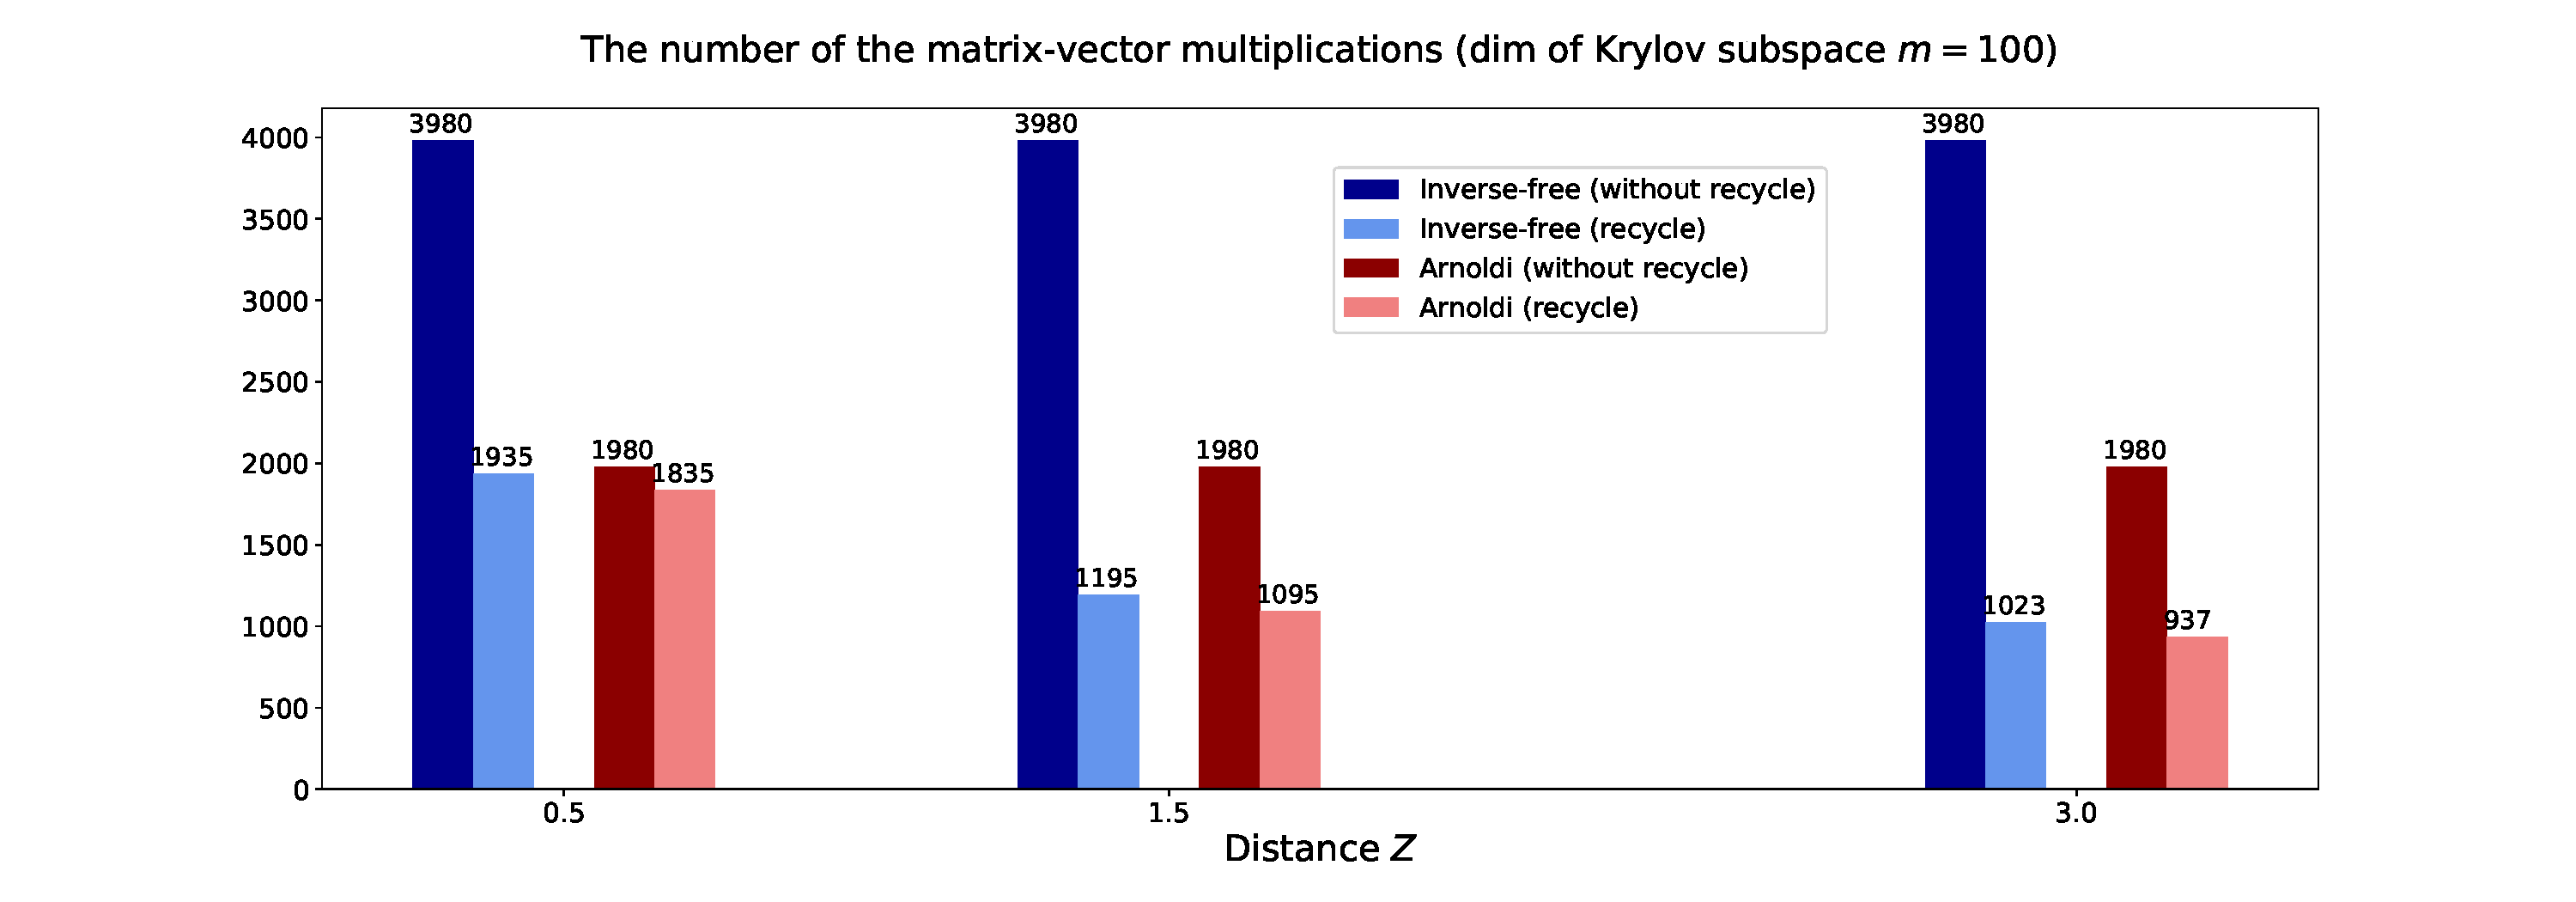
\includegraphics[scale = 0.4]{figures/matvec_100.pdf}
    \caption{The number of the matrix-vector products inside inverse-free and standard Arnoldi methods with or without recycling subspace. The scatterers are two spheres with equal radii $R = 1$ and distance $Z$ is 0.5, 1.5 and 3.0. The dimension of the Krylov subspace is set as $m = 100$.}
    \label{matvec100}
\end{figure}

\begin{figure}[H]
    \centering
    \hspace*{-1.5cm}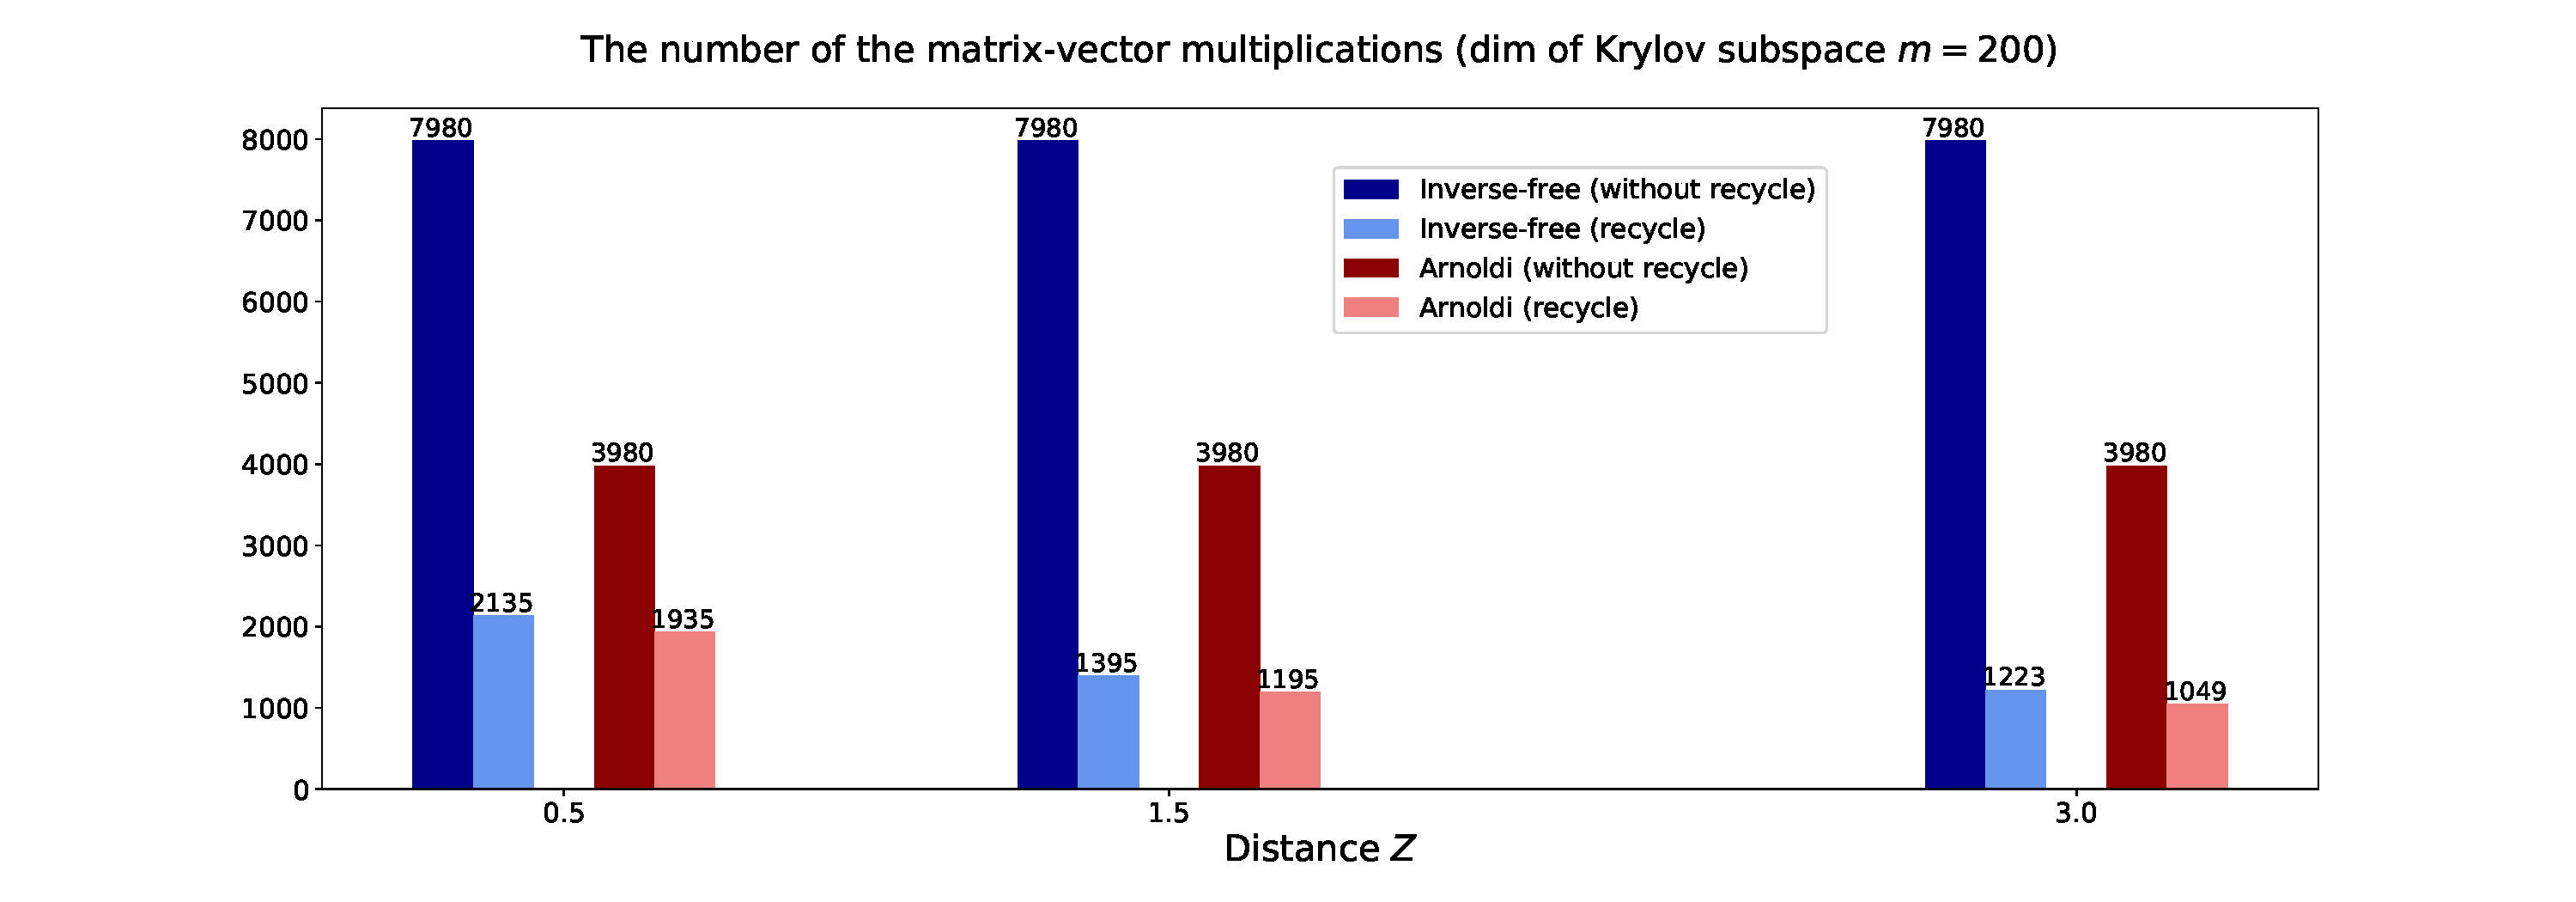
\includegraphics[scale = 0.4]{figures/matvec_200.pdf}
    \caption{The number of the matrix-vector products inside inverse-free and standard Arnoldi methods with or without recycling subspace. The scatterers are two spheres with equal radii $R = 1$ and distance $Z$ is 0.5, 1.5 and 3.0. The dimension of the Krylov subspace is set as $m = 200$.}
    \label{matvec200}
\end{figure}

%Note that for the recycled methods Algorithm \ref{Alg for computing the evals kry recycled}-\ref{Alg for computing the evals arno recycled}
%we apply different rules for extracting the eigenvectors. For  
%is different which depends on the 

%For the standard Arnoldi method,  it can be noticed that the number of FLOP is cubicly increasing with the size of the matrix 
%no matter the subspace is recycled or not. For the inverse-free Krylov subspace methods, as the wavenumber $k$ increases, the number of the extreme eigenvalues
%decreases which makes the number of extracted eigenvectors decreases as well. Therefore, for the large-scale problems, the inverse-free Krylov subspace method with 
%subspaces recycled would be applied to compute the Casimir energy with lower complexity and desired accuracy.


\section{Numerical experiments}\label{Numerical experiments}
In this section, we are going to show the numerical results for computing the Casimir energy between two perfectly conducting objects, which are spheres, 
menger sponges, ice crystals and ellipsoids. The reference value of the Casimir energy is computed by the Richardson extrapolation method which is often used 
for obtaining the higher-order estimate at zero grid spacing. Denote $\mathcal{E}_{\text{fine}}$ and $\mathcal{E}_{\text{coarse}}$ as the Casimir energy 
numerically computed from the formula \eqref{KSSF and CasE} by setting the grid size $h$ as $h_{\text{fine}}$ and $h_{\text{coarse}}$ 
($h_{\text{fine}}<h_{\text{coarse}}$), separately. Then, the high-accuracy result $\mathcal{E}_{\text{exact}}$ can be generated from the following formula:
\begin{align}\label{Richardson extrapolation}
    \mathcal{E}_{\text{exact}} \approx \mathcal{E}_{\text{fine}} + \frac{h_{\text{coarse}}^{2}\mathcal{E}_{\text{fine}} - h_{\text{fine}}^{2}\mathcal{E}_{\text{coarse}}}{h_{\text{coarse}}^{2} - h_{\text{fine}}^{2}}.
\end{align}
In addition, the asymptotic series of the Casimir energy are also available in two spheres' case and the series can be found in \cite{emig2008casimir} 
for both equal and unequal radii's cases. 

\subsection{Two spheres case}
\begin{figure}[H]
    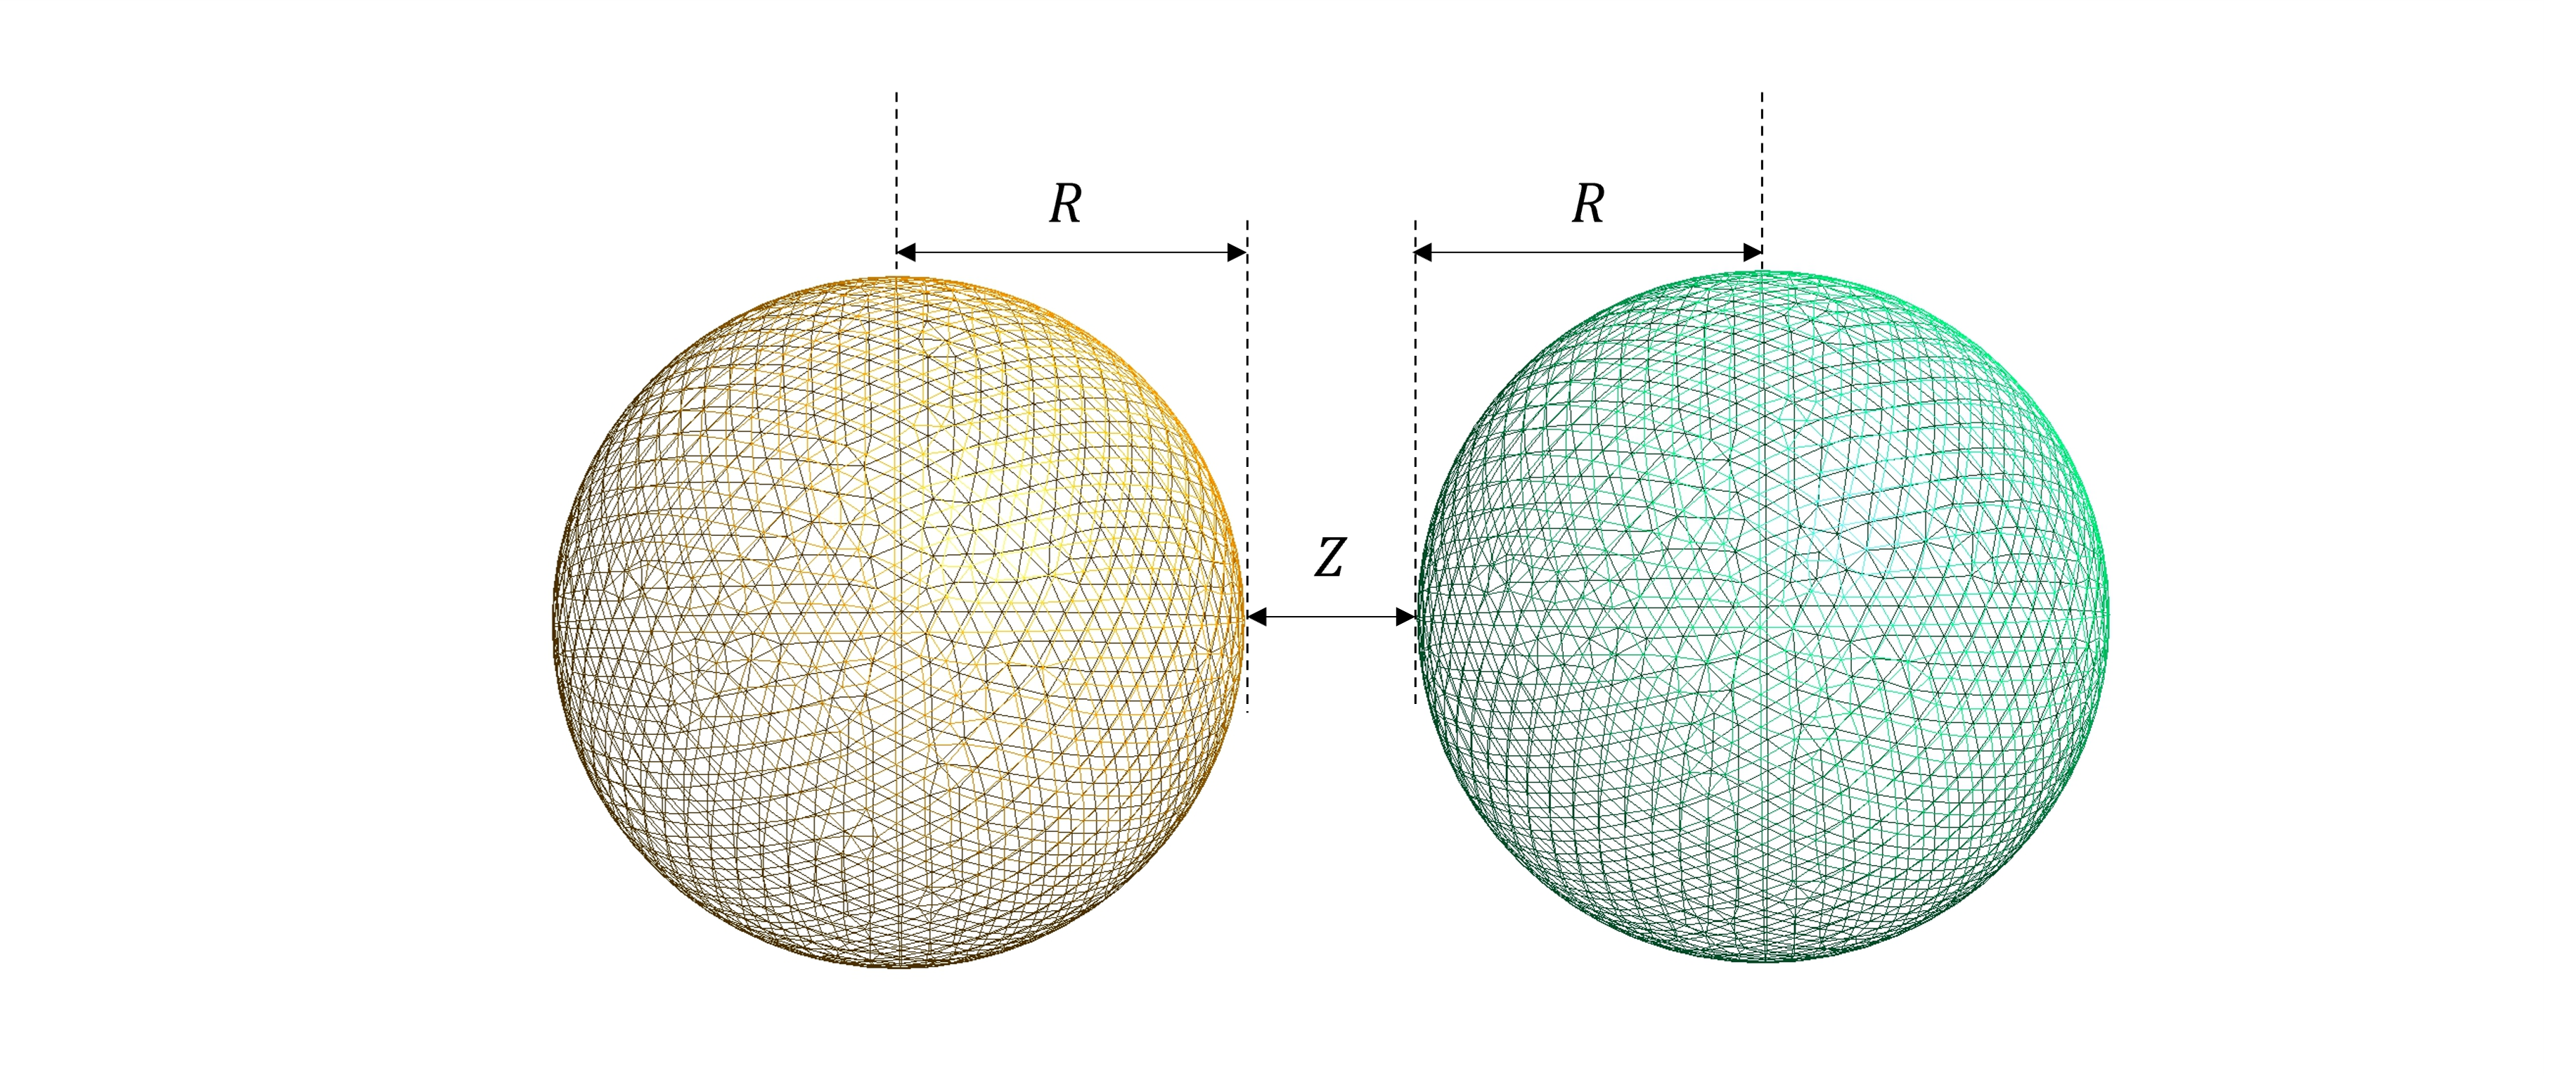
\includegraphics[scale = 0.6]{figures/Grid_two_spheres_dist.png}
    \caption{Two spheres with equal radii: $R$ represents the radius of the spheres and $Z$ is the distance between them.}
    \label{Two spheres with equal radii}
\end{figure}

Consider two perfectly conducting spheres with equal radii, which are shown in the Figure \ref{Two spheres with equal radii}. Inside the figure, $R$ is the radius 
of the spheres and the distance between them is denoted as $Z$. We begin with estimating the Casimir energy between two spheres with radius $R = 1$ at the 
distance of $Z$ via the formula \eqref{KSSF and CasE} in two different refinement levels: $h_{\text{fine}} = 0.05$ and $h_{\text{coarse}} = 0.1$ and the 
distance $Z$ between them is ranging from 0.5 to 3.0. Afterwards, the extrapolation result can be obtained by substituting these Casimir energy estimates into 
the formula \eqref{Richardson extrapolation}. This result would be regarded as the exact value of the Casimir energy and can be used to compare with the 
estimates derived from the asymptotic series introduced below. 

According to \cite{emig2008casimir}, the Casimir energy between two spheres (with equal radii $R$) at asymptotically 
large separations can be obtained as a series in terms of the ratio of centre distance $L$ ($L = 2R + Z$) to sphere radius $R$:
\begin{align}\label{Asymptotic equal radii}
   \mathcal{E} = -\frac{\hbar c}{\pi}\frac{1}{L}\sum_{n=0}^{\infty}b_{n}\left(\frac{R}{L}\right)^{n+2},
\end{align}
where the first six coefficients are 
$b_{0} = -1/4$, $b_{1} = -1/4$,  $b_{2} = -77/48$,  $b_{3} = -25/16$,  $b_{4} = -29837/2880$, $b_{5} = -6491/1152$. Figure 
\ref{Casimir energy between spheres with equal radii} shows the comparison between the Casimir energy computed from asymptotic series 
\eqref{Asymptotic equal radii} and the exact value evaluated through {Richardson extrapolation}. Here, we observe that the asymptotic value gradually 
approaches to the exact value as the distance $Z$ increases since the asymptotic expansion \eqref{Asymptotic equal radii} only works when the distance 
between two spheres is asymptotically large.

\begin{figure}[H]
    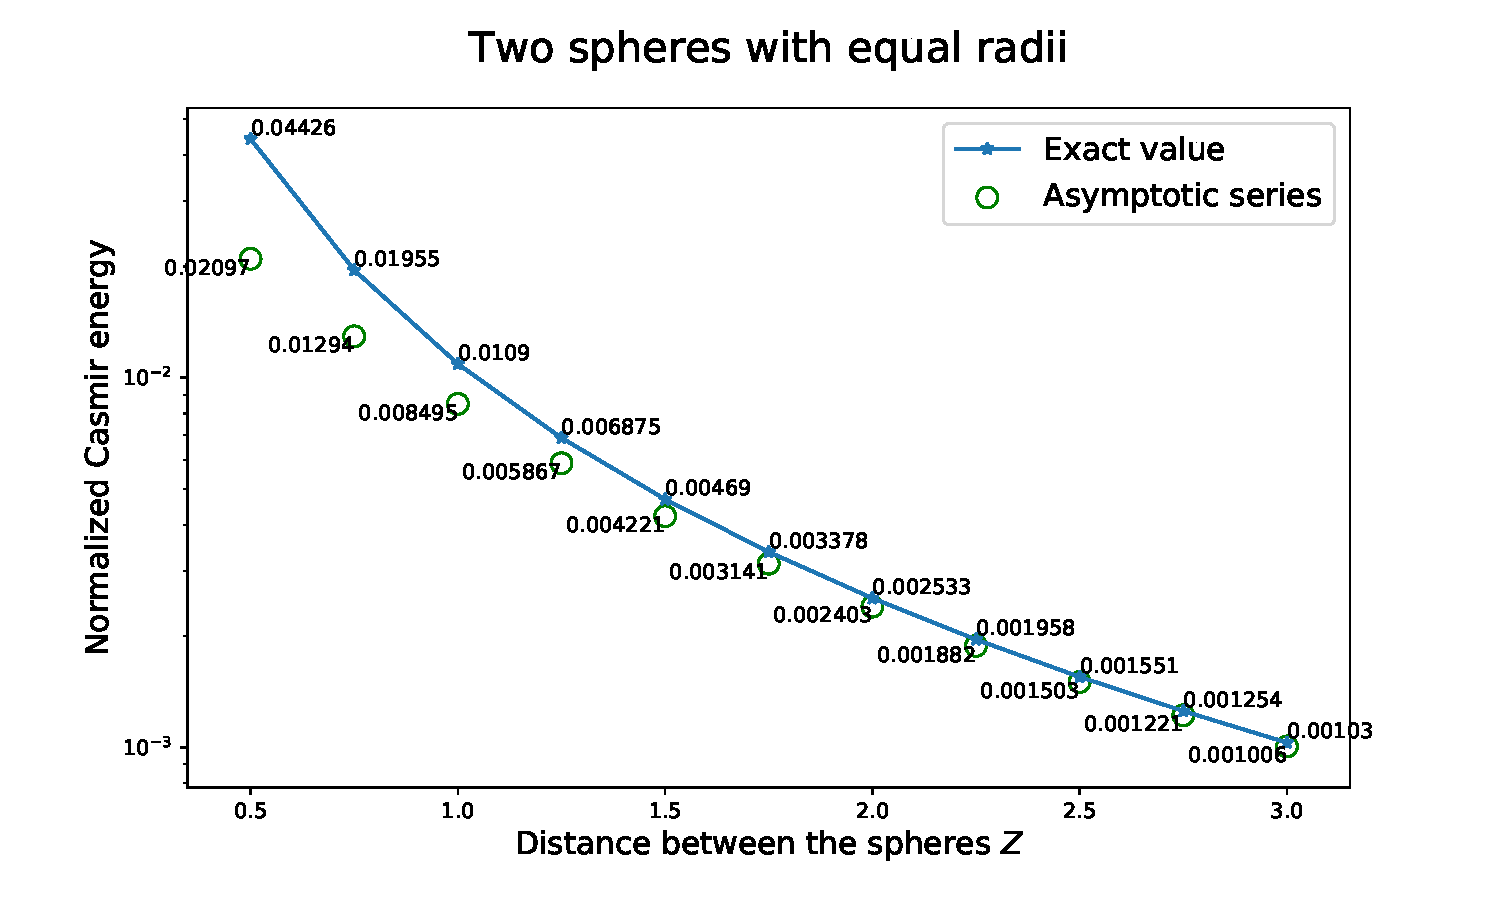
\includegraphics[scale = 0.7]{figures/Spheres_equal_CasE.pdf}
    \caption[Caption for LOF]{Normalized Casimir energy\protect\footnotemark in two spheres with equal radii's case. The radius is $R = 1$ and the distance $Z$ 
    ranges from 0.5 to 3.0. The exact value of the (normalized) Casimir energy has been written beside the data point, which is round up to 4 significant digits.}
    \label{Casimir energy between spheres with equal radii}
\end{figure}
\footnotetext{The normalized Casimir energy is $\mathcal{E}/\hbar c$, for $\mathcal{E}$ defined in \eqref{KSSF and CasE}.}

Afterwards, in order to test the performance of the two efficient methods introduced in Section \ref{Krylov subspace for generalized eigenvalue problem}, we
would use them to evaluate the Casimir energy between two spheres described above. For the inverse-free Krylov subspace method, the dimension of the Krylov subspace is set as $m = 20$ and 50 and the 
number of approximated smallest (or largest) eigenvalues is $p = 10$ and 25, respectively. For the standard Arnoldi method, the dimension of the 
Krylov subspace is also set as $m = 20$ and 50. 

Figure \ref{equal_radii_rel_dist} shows the relative distance between the estimates computed through inverse-free Krylov subspace method 
(dashed/solid green triangles), standard Arnoldi method (dashed/solid blue circles), asymptotic series (solid black square) and the exact values.
Here, we can easily see that the inverse-free Krylov subspace method behaves better than the standard Arnoldi method no matter when the dimension $m$ is 
20 or 50 and as we increase the Krylov subspace dimension, the relative error decreases.

In addition, it can be noticed that when the distance $Z$ between the spheres increases, the relative error 
for both methods goes down. The reason appears to be that the cross interaction between them becomes weaker as the spheres are getting away from each other. 
This leads the compact perturbation $\tilde{\mathsf{V}}_{k}$ to become close to $\mathsf{V}_{k}$, which reduces the number of the eigenvalues that mainly 
contribute on the log determinant of $\mathsf{V}_{k}\tilde{\mathsf{V}}_{k}^{-1}$. Therefore, if we keep setting the same dimension of Krylov subspace 
for the spheres are at a large distance, we would have a better approximation on the Casimir energy.


\begin{figure}[H]
    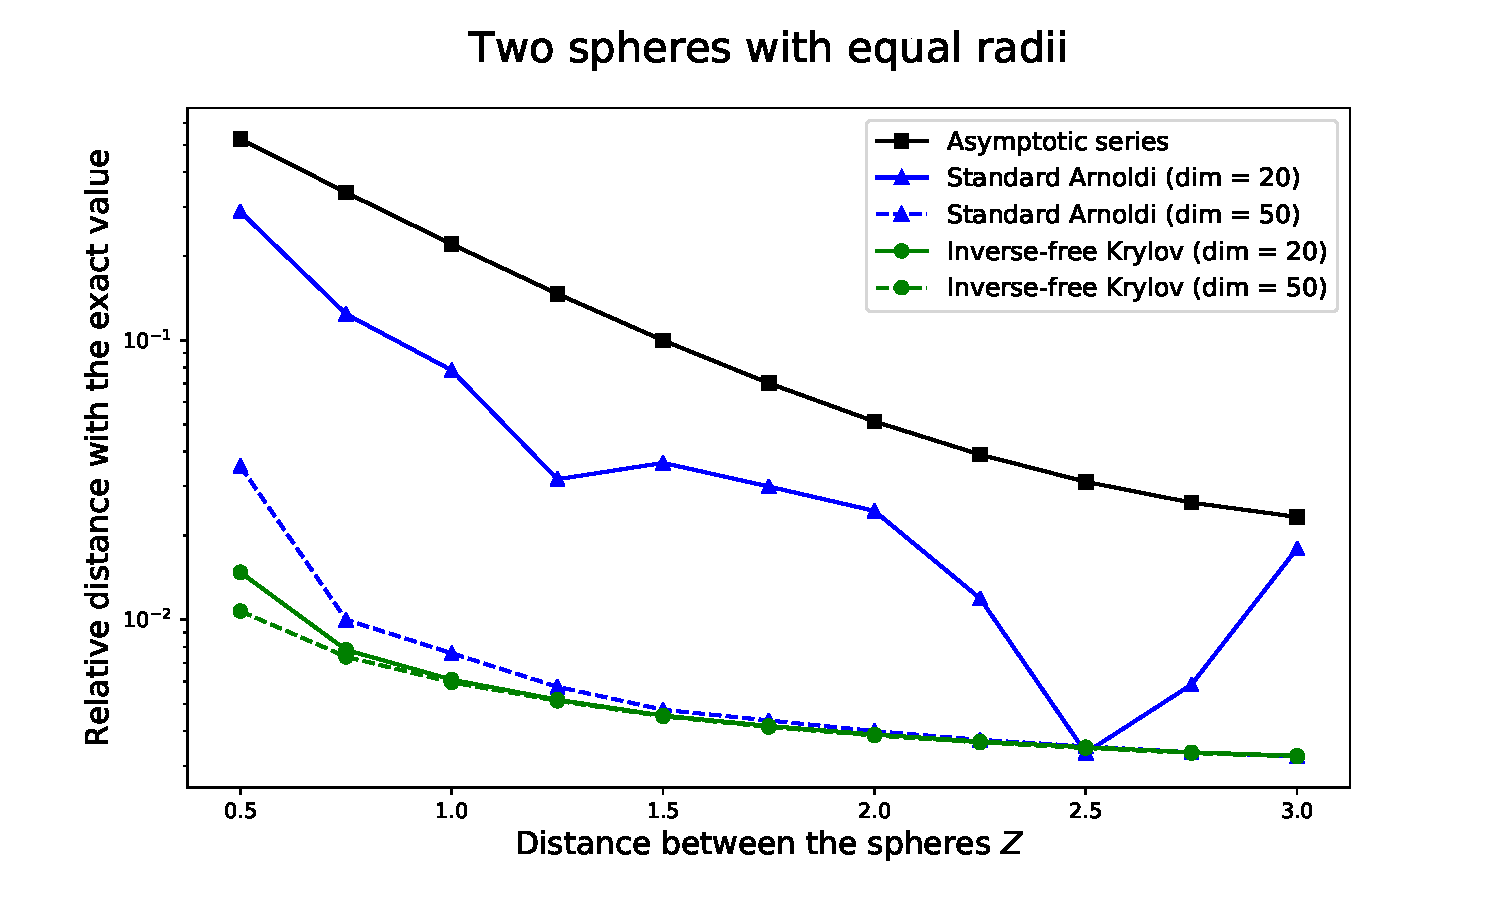
\includegraphics[scale = 0.7]{figures/relative_distance_equal_radii.pdf}
    \caption{Relative distance between the reference value (computed by Richardson extrapolation) with the asymptotic series (solid black square)  
    and the estimates evaluated from the standard Arnoldi method (dashed/solid blue circles) and inverse-free Krylov subspace method (dashed/solid green triangles) 
    by setting the dimension of the Krylov subspace as $m = 20$ and 50 and for the inverse-free
    Krylov subspace method, the number of the approximated smallest (or largest) eigenvalues is set as $p = 10$ and 25, respectively.}
    \label{equal_radii_rel_dist}
\end{figure}
 
%================================================================================================================
\begin{figure}[H]
    \hspace*{2cm}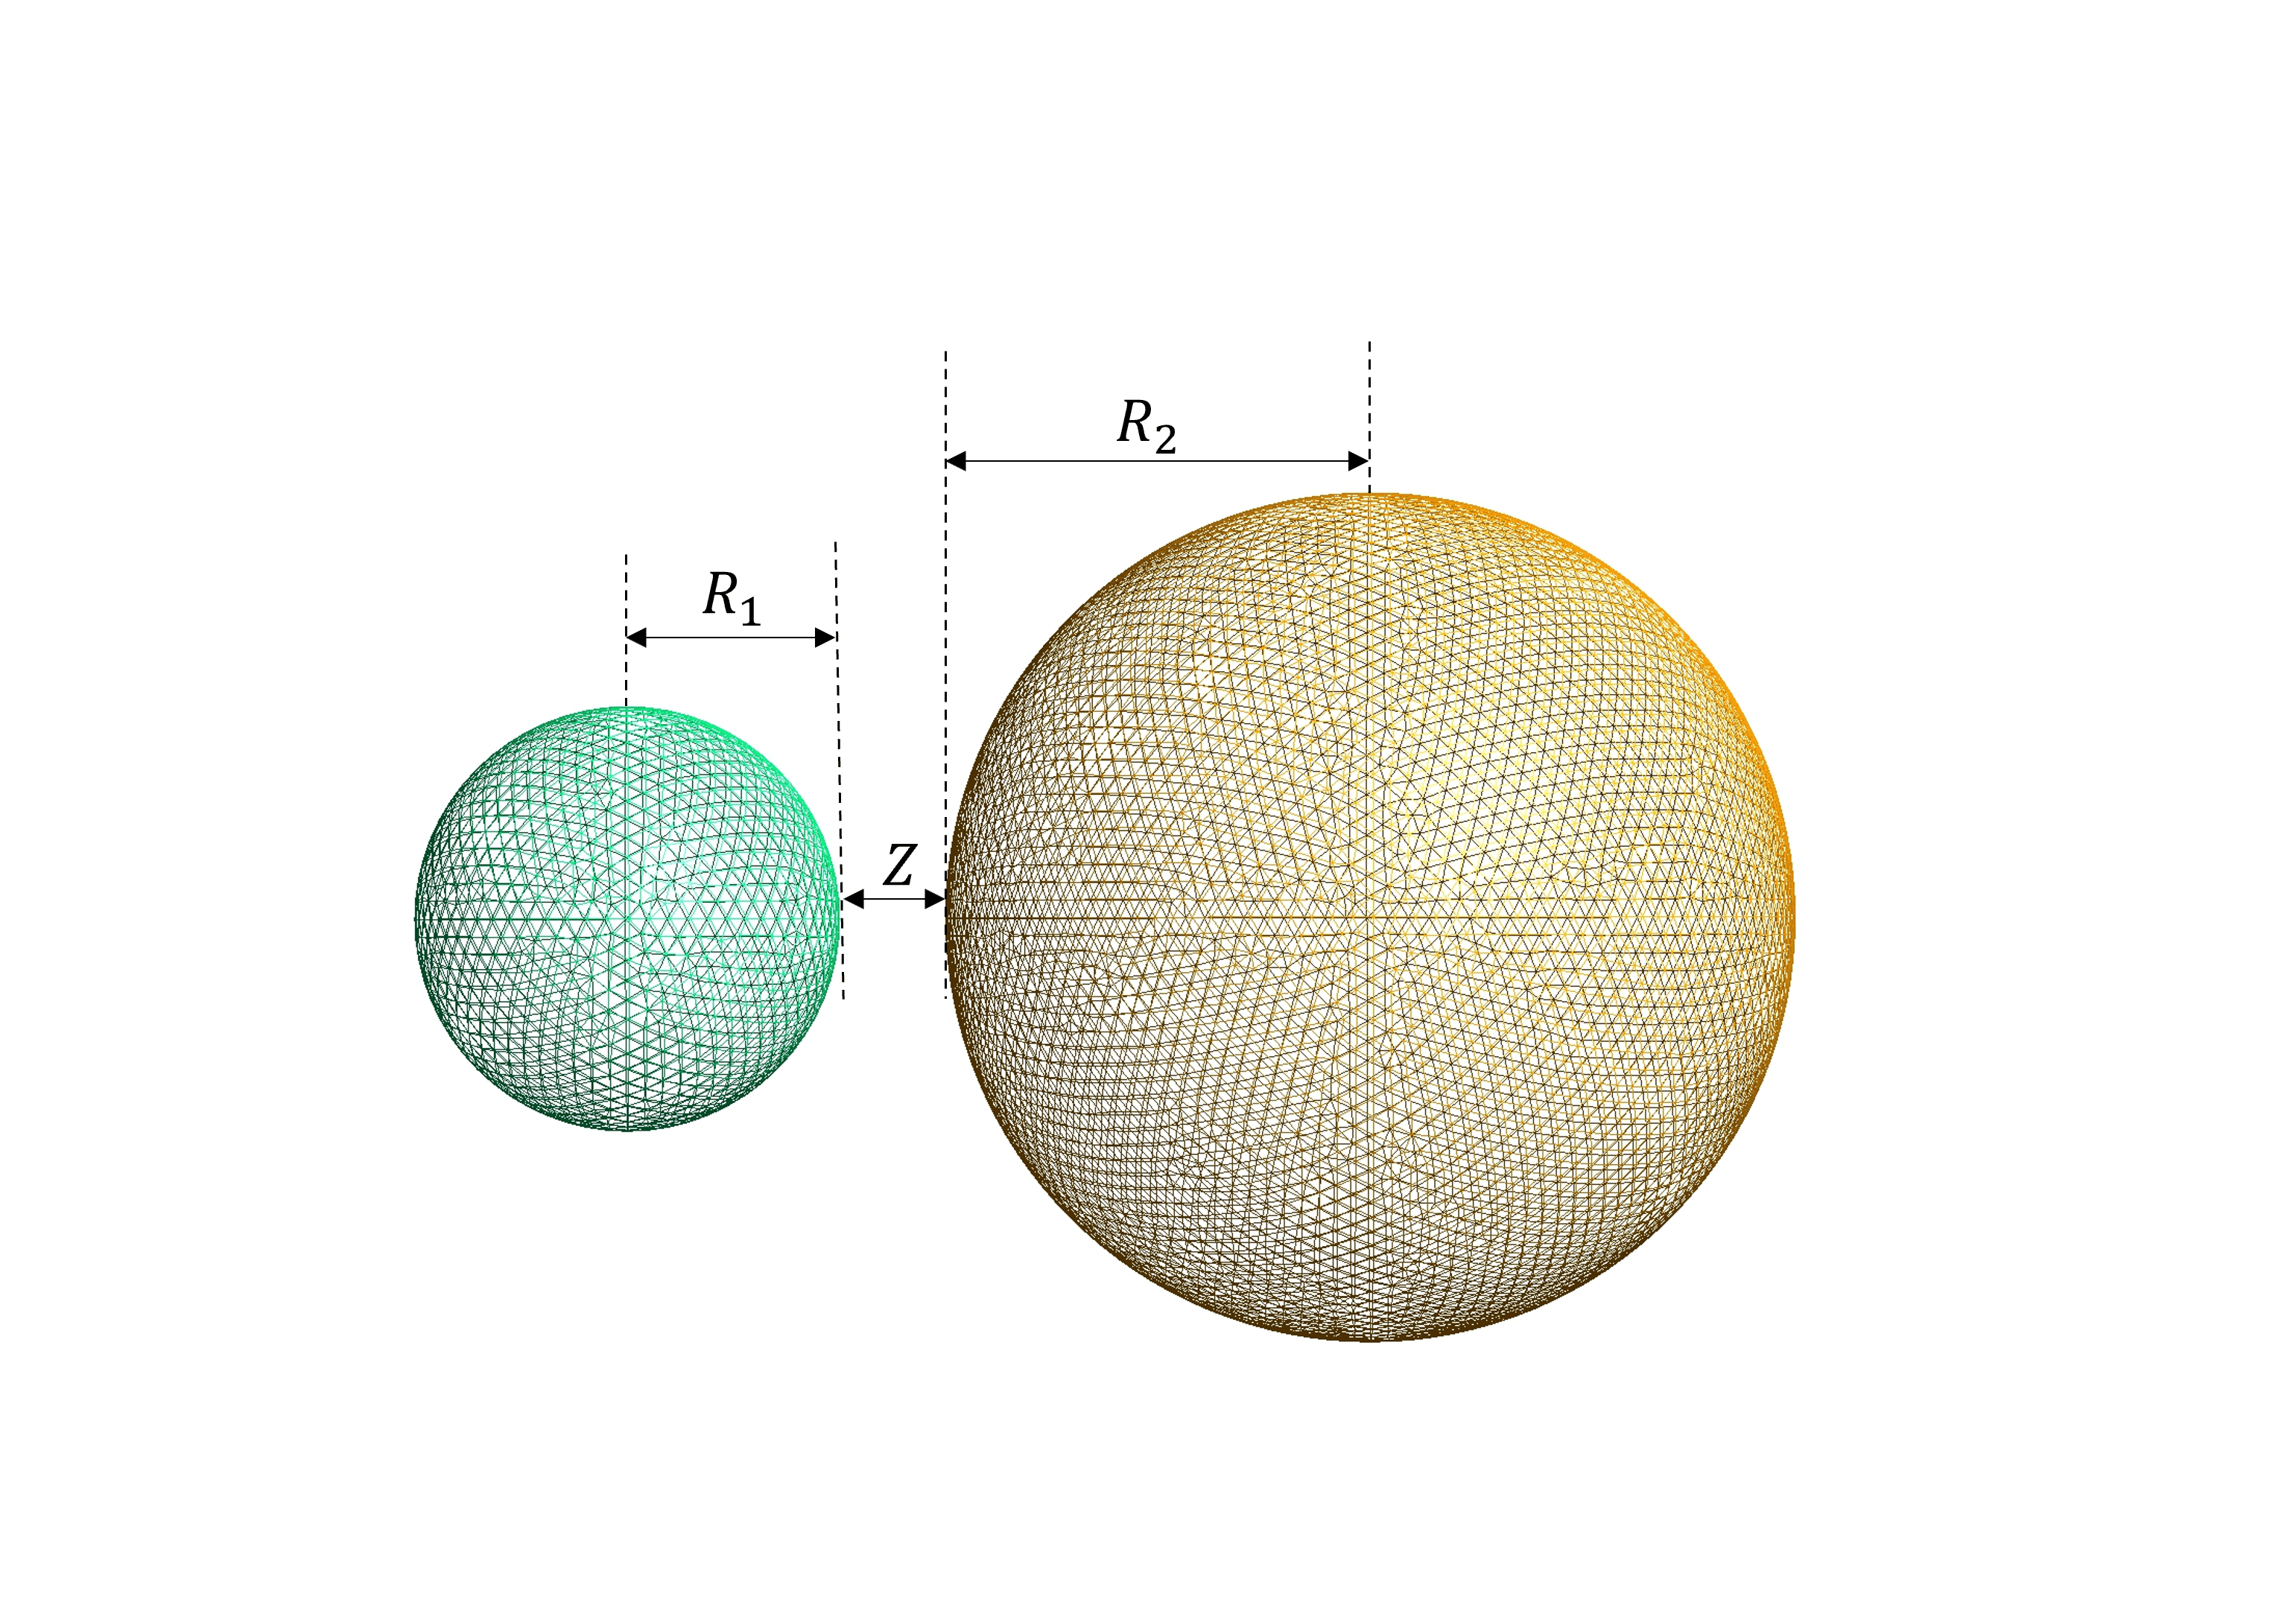
\includegraphics[scale = 0.6]{figures/Grid_two_spheres_unequal_radii.png}
    \caption{Two spheres with unequal radii: $R_{1}$ and $R_{2}$ represent the radius of the spheres and $Z$ is the distance between them.}
    \label{Two spheres with unequal radii}
\end{figure}

When the perfectly conducting spheres have different radii $R_{1}$, $R_{2}$ (see Figure \ref{Two spheres with unequal radii}) and the centre distance is denoted as
$L = R_{1} + R_{2} + Z$, the asymptotic expansion of the Casimir energy at asymptotically large distance can be written as:
\begin{align}\label{Asymptotic unequal radii}
    \mathcal{E} = -\frac{\hbar c}{\pi}\frac{1}{L}\sum_{n=0}^{\infty}\tilde{b}_{n}(\eta)\left(\frac{R_{1}}{L}\right)^{n+2},
\end{align}
where the coefficients $\{\tilde{b}_{n}\}$ depend on the parameter $\eta = R_{2}/R_{1}$ and the first six coefficients are
\begin{align*}
    \tilde{b}_{0} &= -\frac{\eta}{4}, \ \ \ \ \ \tilde{b}_{1} = -\frac{\eta + \eta^{2}}{8}, \ \ \ \ \  \tilde{b}_{2} = -\frac{34(\eta+\eta^{3})+ 9\eta^{2}}{48}, \ \ \ \ \ \tilde{b}_{3} = -\frac{2(\eta+\eta^{4}) + 23(\eta^{2} + \eta^{3})}{32}, \\ 
    \tilde{b}_{4} &= -\frac{8352(\eta + \eta^{5})+ 1995(\eta^{2} + \eta^{4}) + 38980\eta^{3}}{5760}, \ \ \ \ \ \tilde{b}_{5} = -\frac{-1344(\eta+\eta^{6}) + 5478(\eta^{2} + \eta^{5})+2357(\eta^{3} + \eta^{4})}{2304}.
\end{align*}

In the following experiment, the radii of the spheres shown in Figure \ref{Two spheres with unequal radii} are set as $R_{1} = 0.5$ and $ R_{2} = 1$. 
As in the previous example, the exact value of the Casimir energy is computed through the Richardson extrapolation formula \eqref{Richardson extrapolation}, 
where the coarse and fine grid size are $h_{\text{coarse}} = 0.1$ and $h_{\text{fine}} = 0.05$, separately. In this case, the asymptotic value of the Casimir 
energy was estimated by the series \eqref{Asymptotic unequal radii} and the comparison between the exact value and asymptotic one is shown in Figure 
\ref{Casimir energy between spheres with unequal radii}. Again we see that when the distance between two spheres decreases, the asymptotic value gets 
close to the exact one and the reason for this is clearly stated in the above equal radii's case.
\begin{figure}[H]
    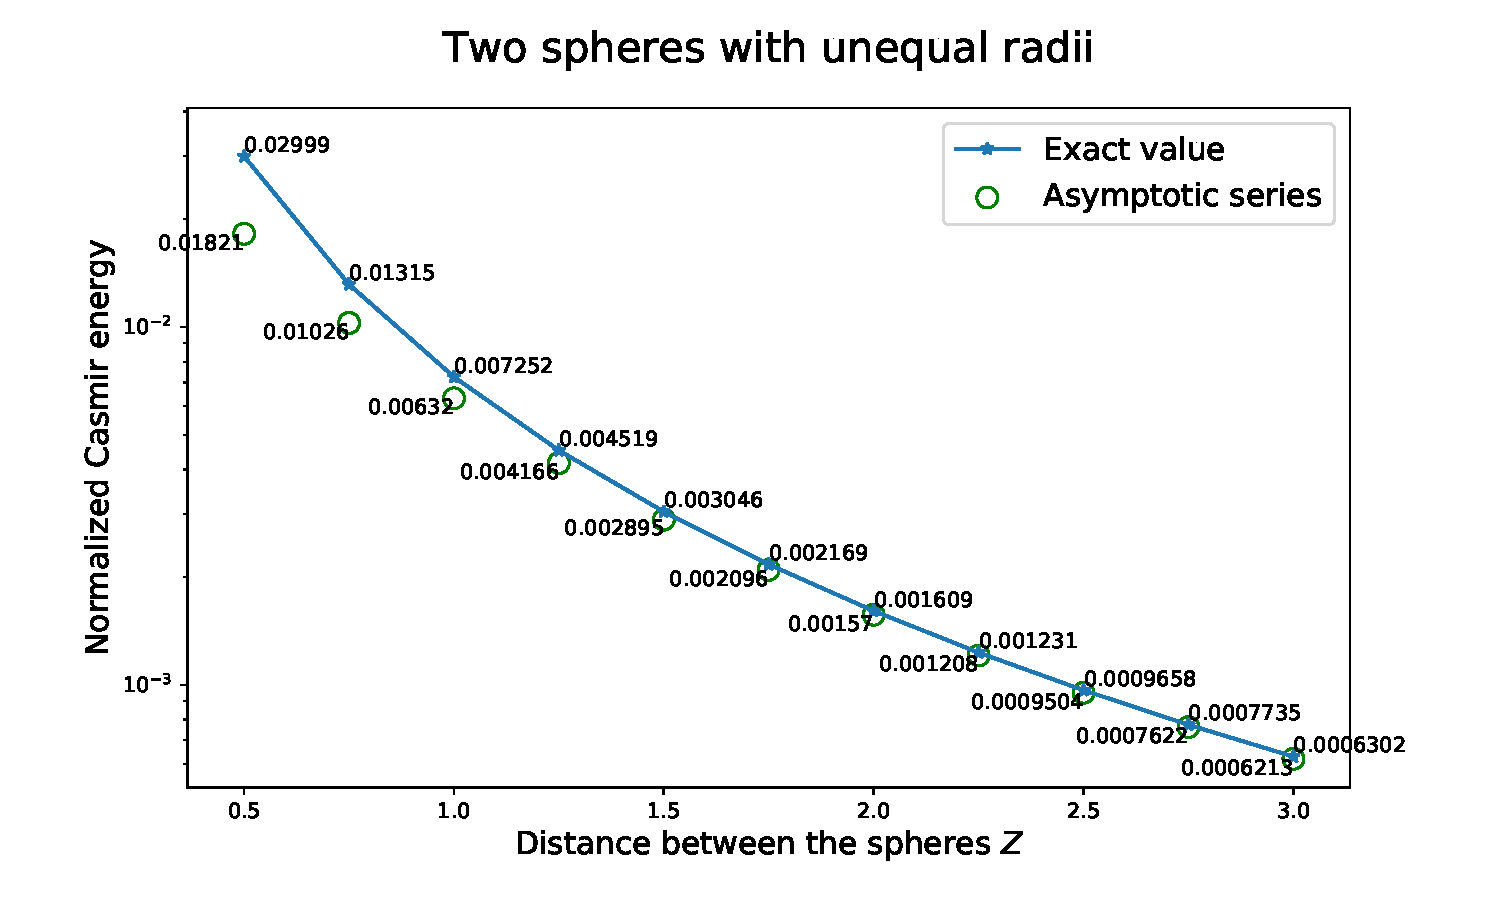
\includegraphics[scale = 0.7]{figures/Spheres_unequal_CasE.pdf}
    \caption{Normalized Casimir energy in two spheres with unequal radii's case. The radius is $R = 1$ and the distance $Z$ 
    ranges from 0.5 to 3.0. The exact value of the (normalized) Casimir energy has been written 
    beside the data point, which is round up to 4 significant digits.}
    \label{Casimir energy between spheres with unequal radii}
\end{figure}

By keeping all the experimental settings being the same with the equal radii's case, the numerical experiments on testing the performance of the inverse-free and 
standard Arnoldi methods have been done in the unequal radii's case and the results are shown in Figure \ref{unequal_radii_rel_dist}, from which we observe that 
the results between these two efficient methods have no big difference except the standard Arnoldi case when the dimension $m = 20$.  Compared with the previous
case, it is supposed to be due to the smaller scatterer, leading to the smaller number of eigenvalues that makes significant influence on the log determinant.

\begin{figure}[H]
    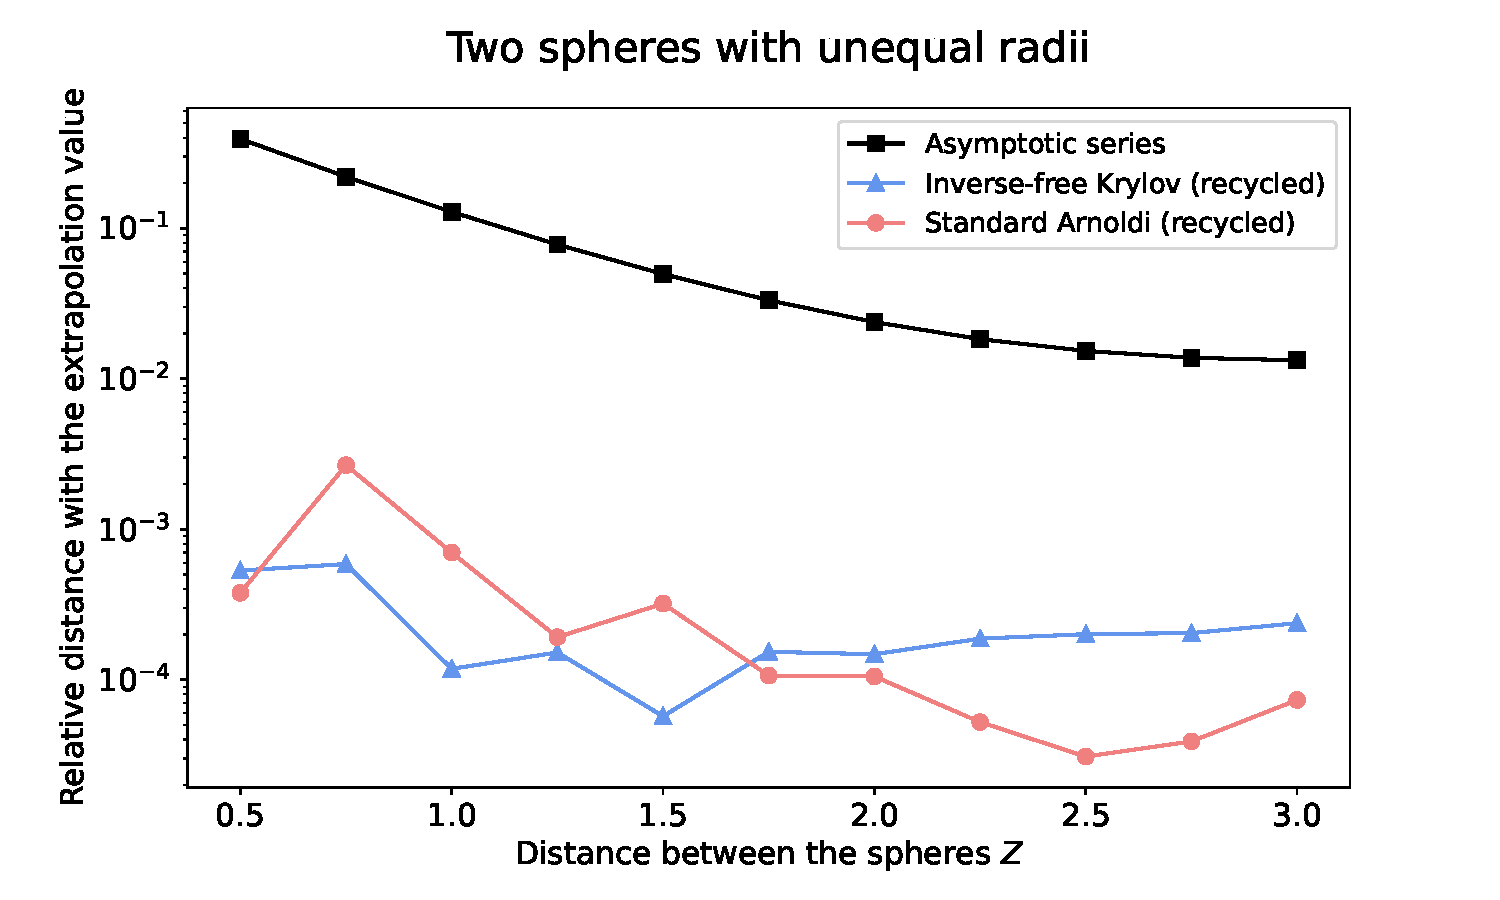
\includegraphics[scale = 0.7]{figures/relative_distance_unequal_radii.pdf}
    \caption{Relative distance between the reference value (computed by Richardson extrapolation) with the asymptotic series (solid black square)  
    and the estimates evaluated from the standard Arnoldi method (dashed/solid blue circles) and inverse-free Krylov subspace method (dashed/solid green triangles) 
    by setting the dimension of the Krylov subspace as $m = 20$ and 50 and for the inverse-free
    Krylov subspace method, the number of the approximated smallest (or largest) eigenvalues is set as $p = 10$ and 25, respectively.}
    \label{unequal_radii_rel_dist}
\end{figure}

\subsection{Realistic objects case}
In this part, the Casimir energy between the objects with special shapes such as the menger sponges, ice crystals and ellipsoids will be computed and 
the values labelled in the following figures are always round up to 4 significant digits. 

Figure \ref{Menger sponges} plots the menger sponges in different levels $(0, 1 $ and $ 2)$ and the length of these sponges is always 1. Afterwards, the Casimir 
energy between two menger sponges in the same level are plotted in Figure \ref{Normalized Casimir energy in two menger sponges' case}. By comparing the data 
point in these subfigures, it is easy to find that the Casimir energy decreases as the number of the iteration increases since the cross-sectional 
area gets smaller.

\begin{figure}[H]
    \centering
    \subfloat[Level 0]{{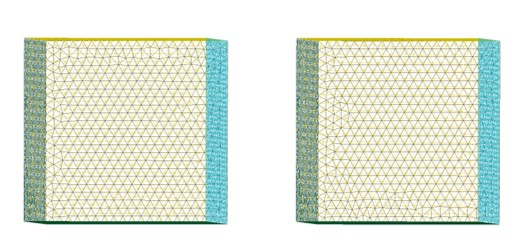
\includegraphics[width=0.4\textwidth]{figures/merger_sponge_level0.jpg} }}
    \qquad
    \subfloat[Level 1]{{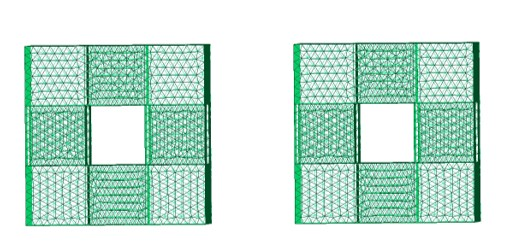
\includegraphics[width=0.4\textwidth]{figures/merger_sponge_level1.jpg} }}
    \qquad
    \subfloat[Level 2]{{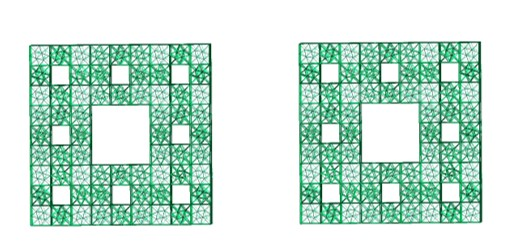
\includegraphics[width=0.4\textwidth]{figures/merger_sponge_level2.jpg} }}
    \caption{Menger sponges in different levels. The length of each sponge is 1.}
    \label{Menger sponges}
\end{figure}

\begin{figure}[H]
    \centering
    \hspace*{-1.5cm}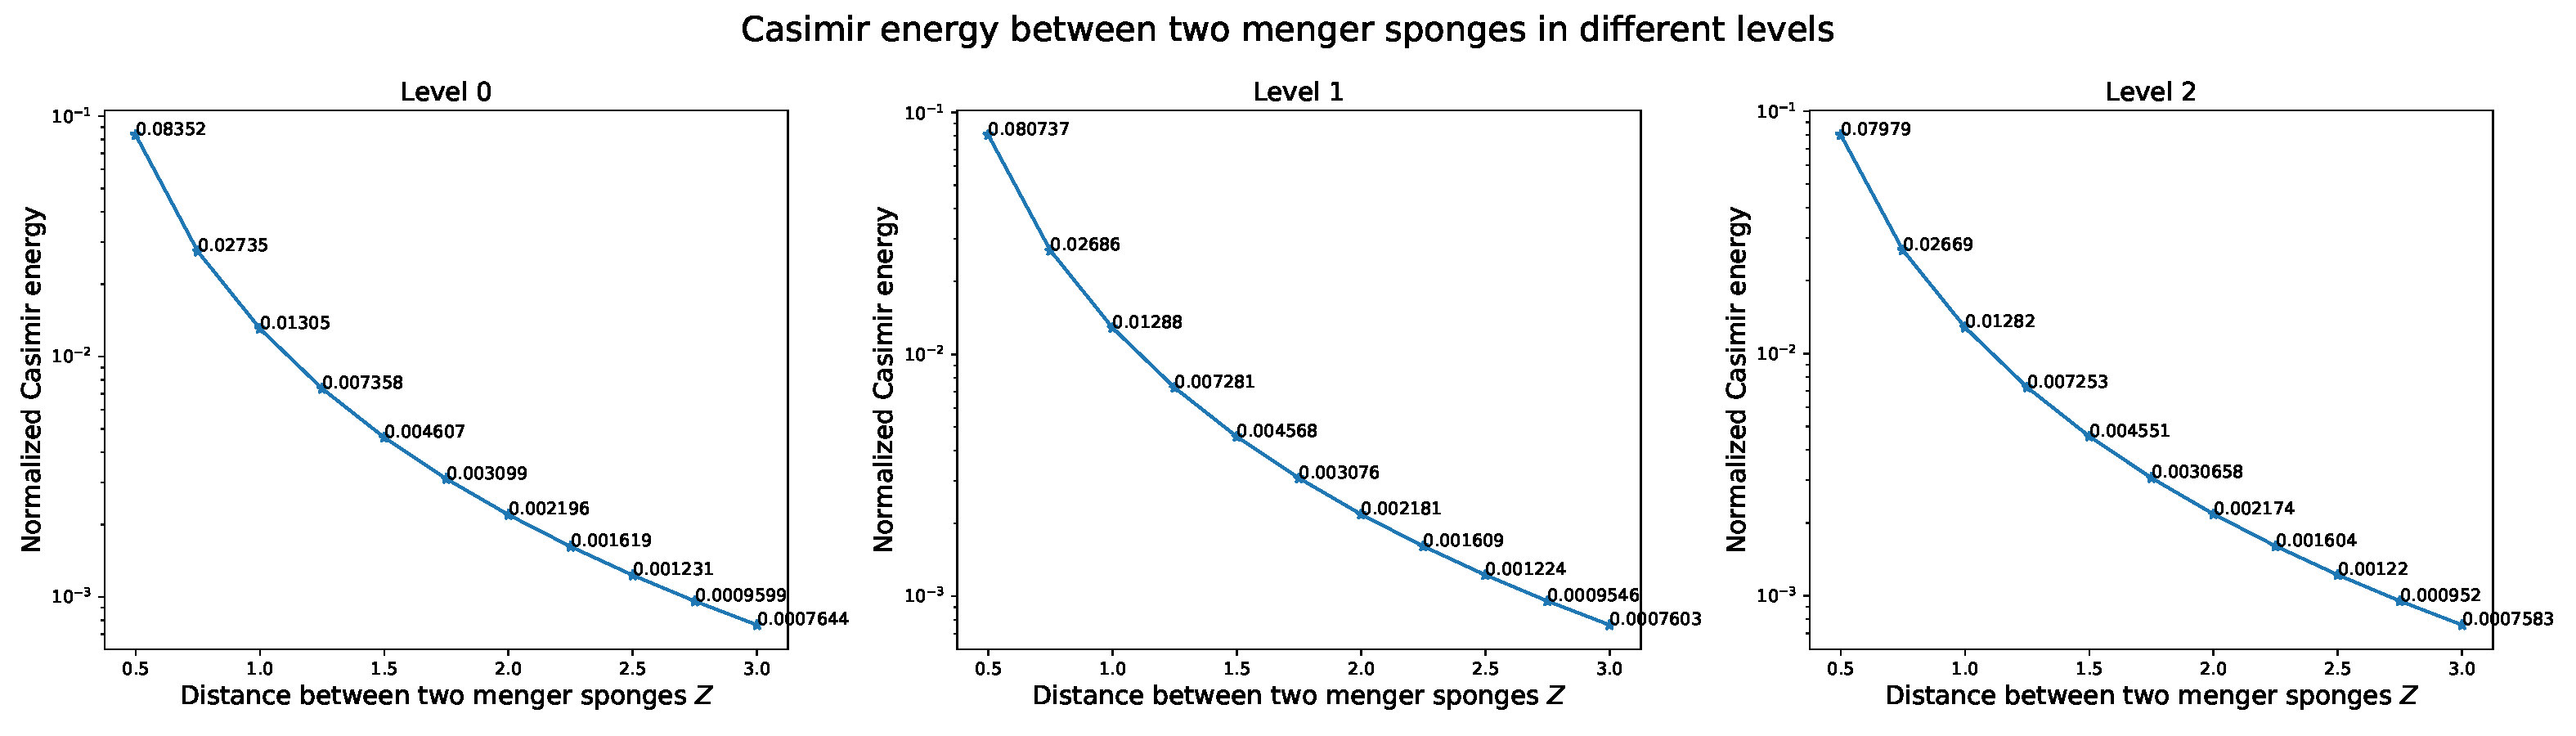
\includegraphics[width=1.2\textwidth]{figures/Cas_menger_spongers.pdf}
    \caption{Normalized Casimir energy in two menger sponges' case. The length of each sponge is 1.}
    \label{Normalized Casimir energy in two menger sponges' case}
\end{figure}
%==========================================================================================
In the next example, the scatterers are ice crystals with different number of branches ranging from 2 to 6 (see Figure \ref{Ice crystals with different number of branches}).
By Figure \ref{Normalized Casimir energy in ice crystals' case}, when the number of branches increases from 2 to 4, the Casimir energy increases as expected. But 
when the branches number added up to 5 and 6, the Casimir energy is much smaller since the main cross-sectional part cannot be as close as the 
2, 3, 4-branches cases. 

\begin{figure}[H]
    \begin{subfigure}{0.3\linewidth}
        \centering
        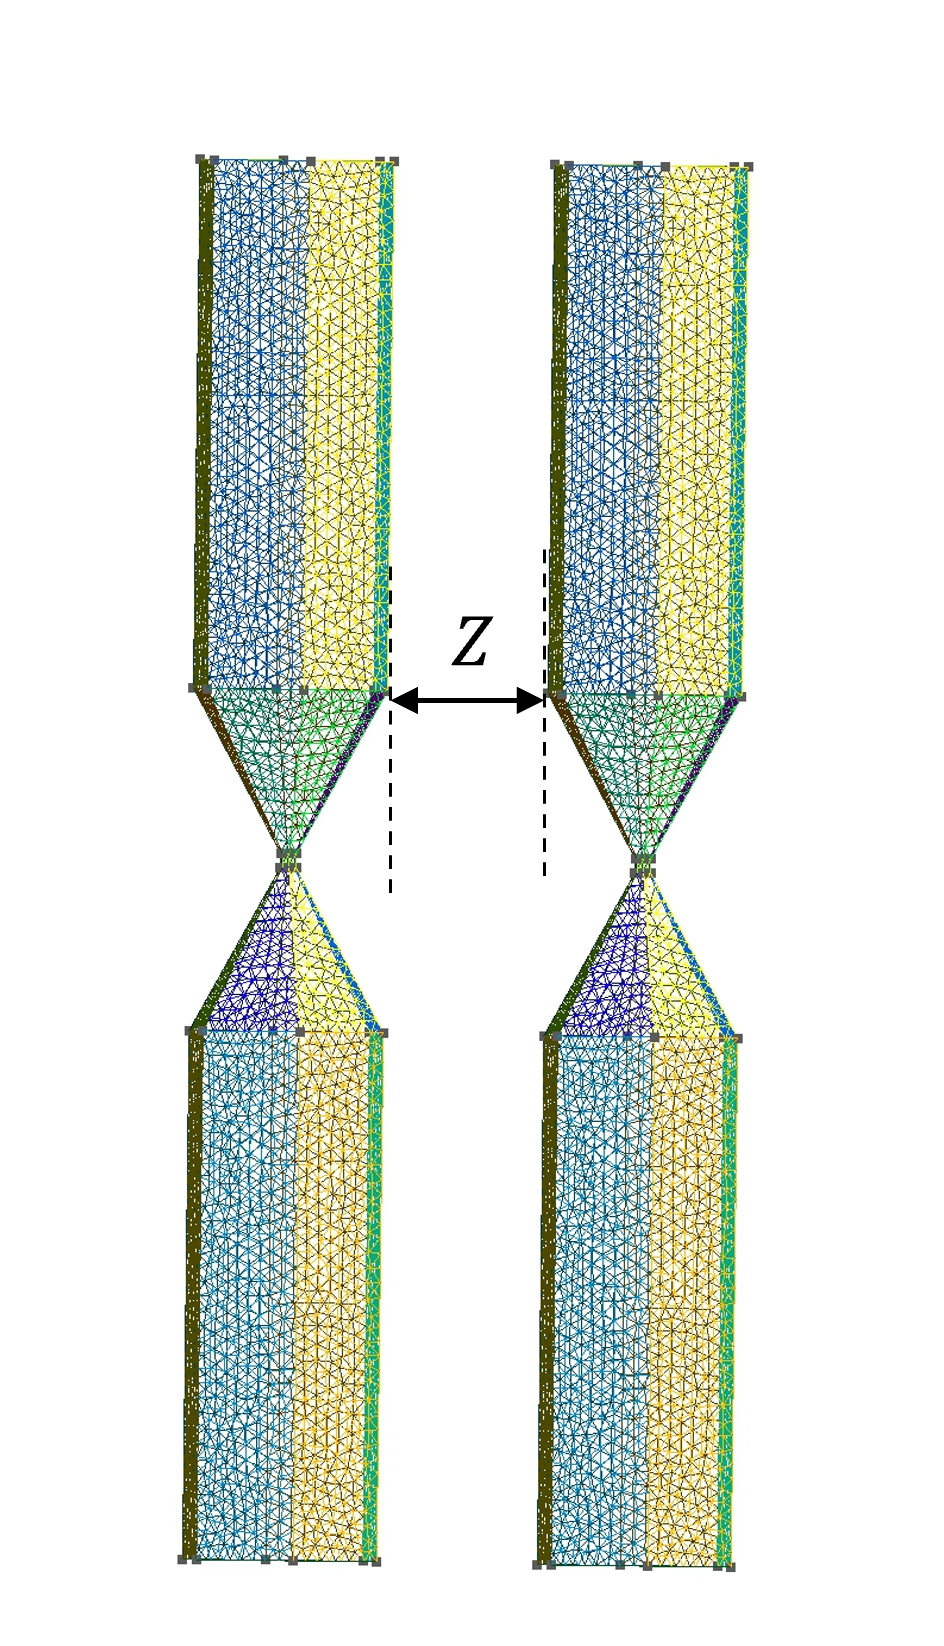
\includegraphics[scale = 0.4]{figures/2branches}
        \caption{Two branches}
        \end{subfigure}
        \begin{subfigure}{0.3\linewidth}
            \centering
            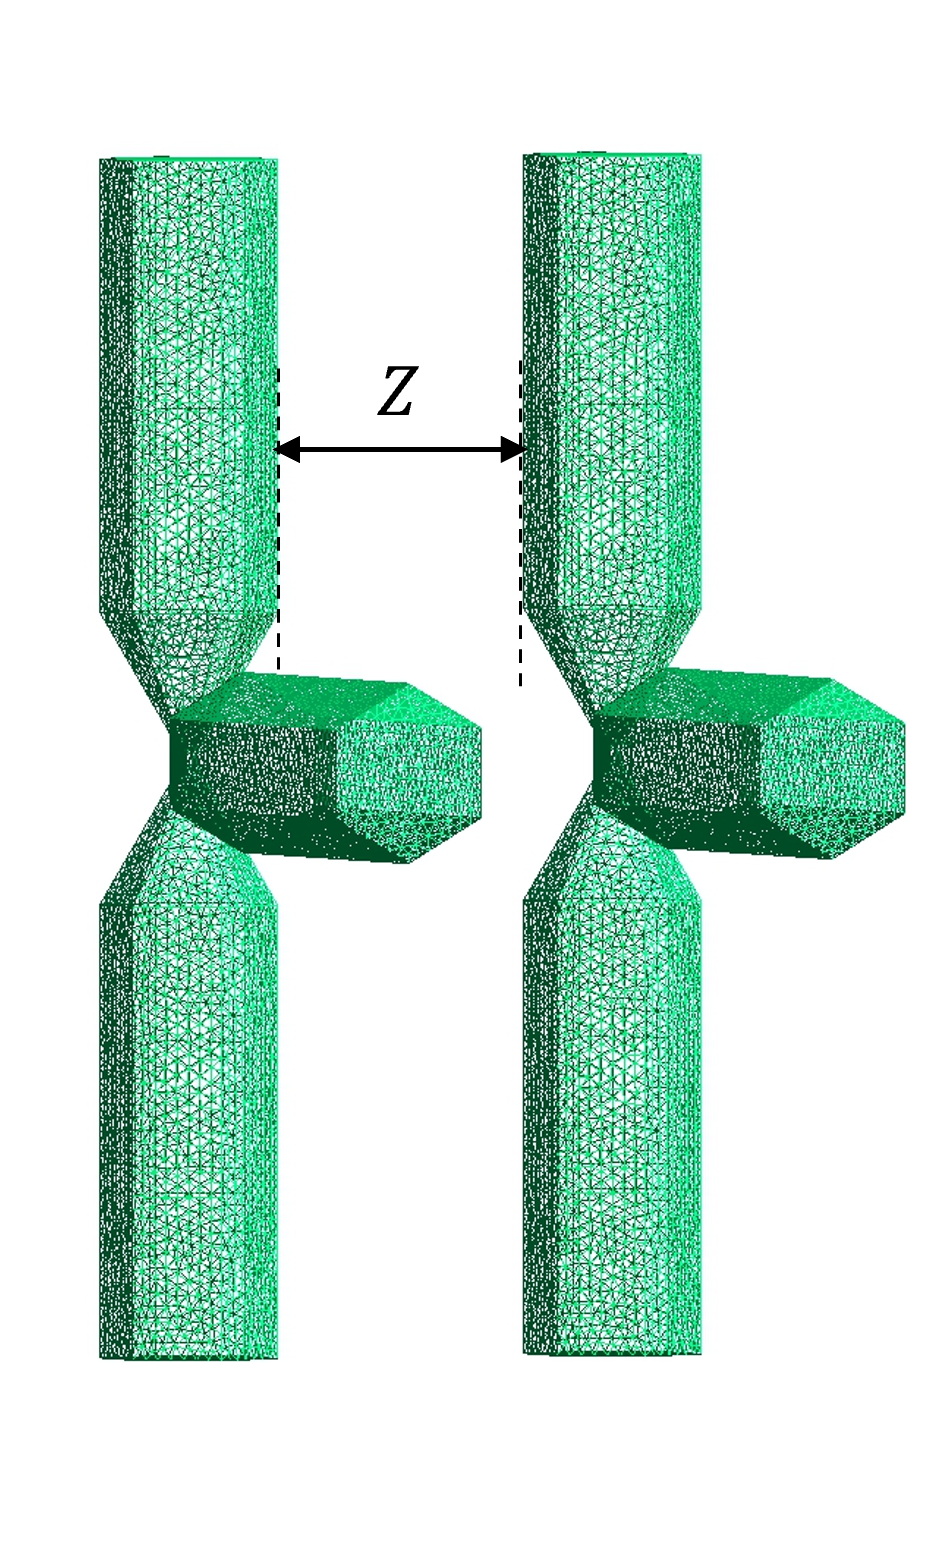
\includegraphics[scale = 0.4]{figures/3branches}
            \caption{Three branches}
            \end{subfigure}
            \begin{subfigure}{0.3\linewidth}
                \centering
                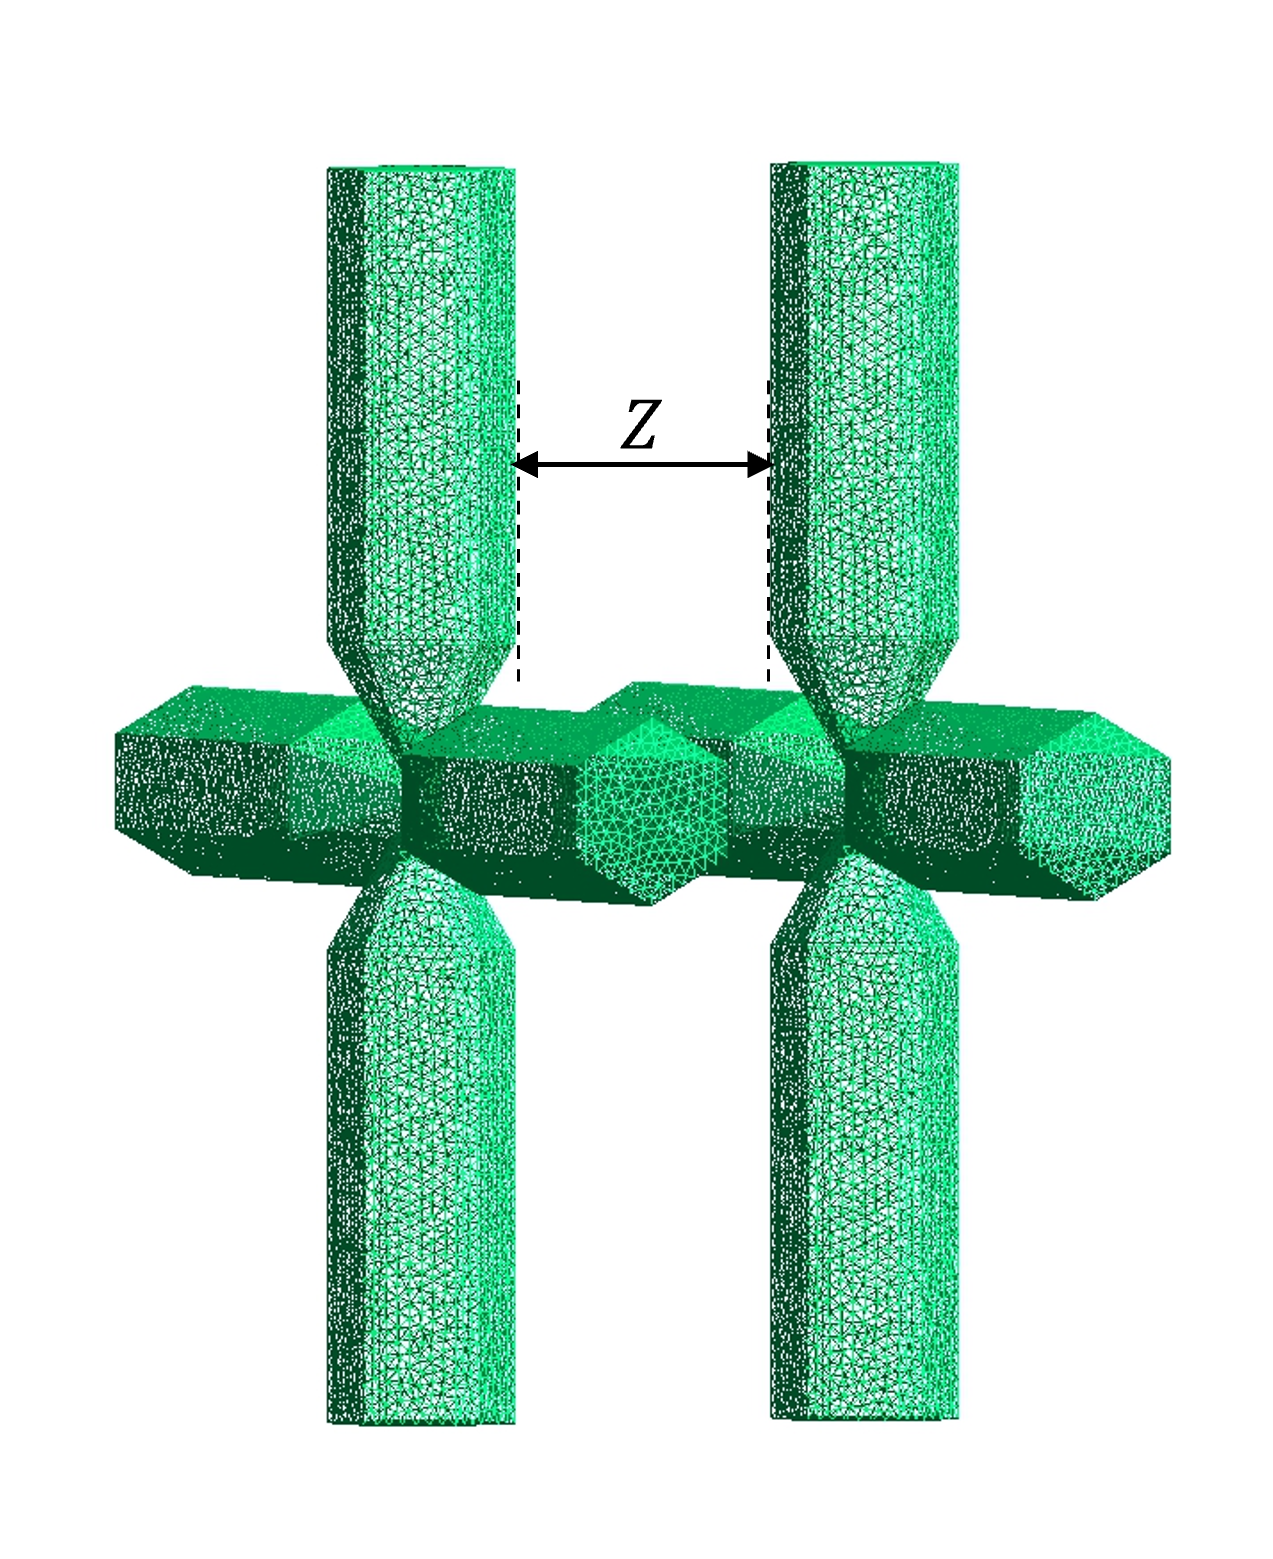
\includegraphics[scale = 0.38]{figures/4branches}
                \caption{Four branches}
                \end{subfigure}\\[1ex]
    \begin{subfigure}{.5\linewidth}
    \centering
    \hspace*{-1cm}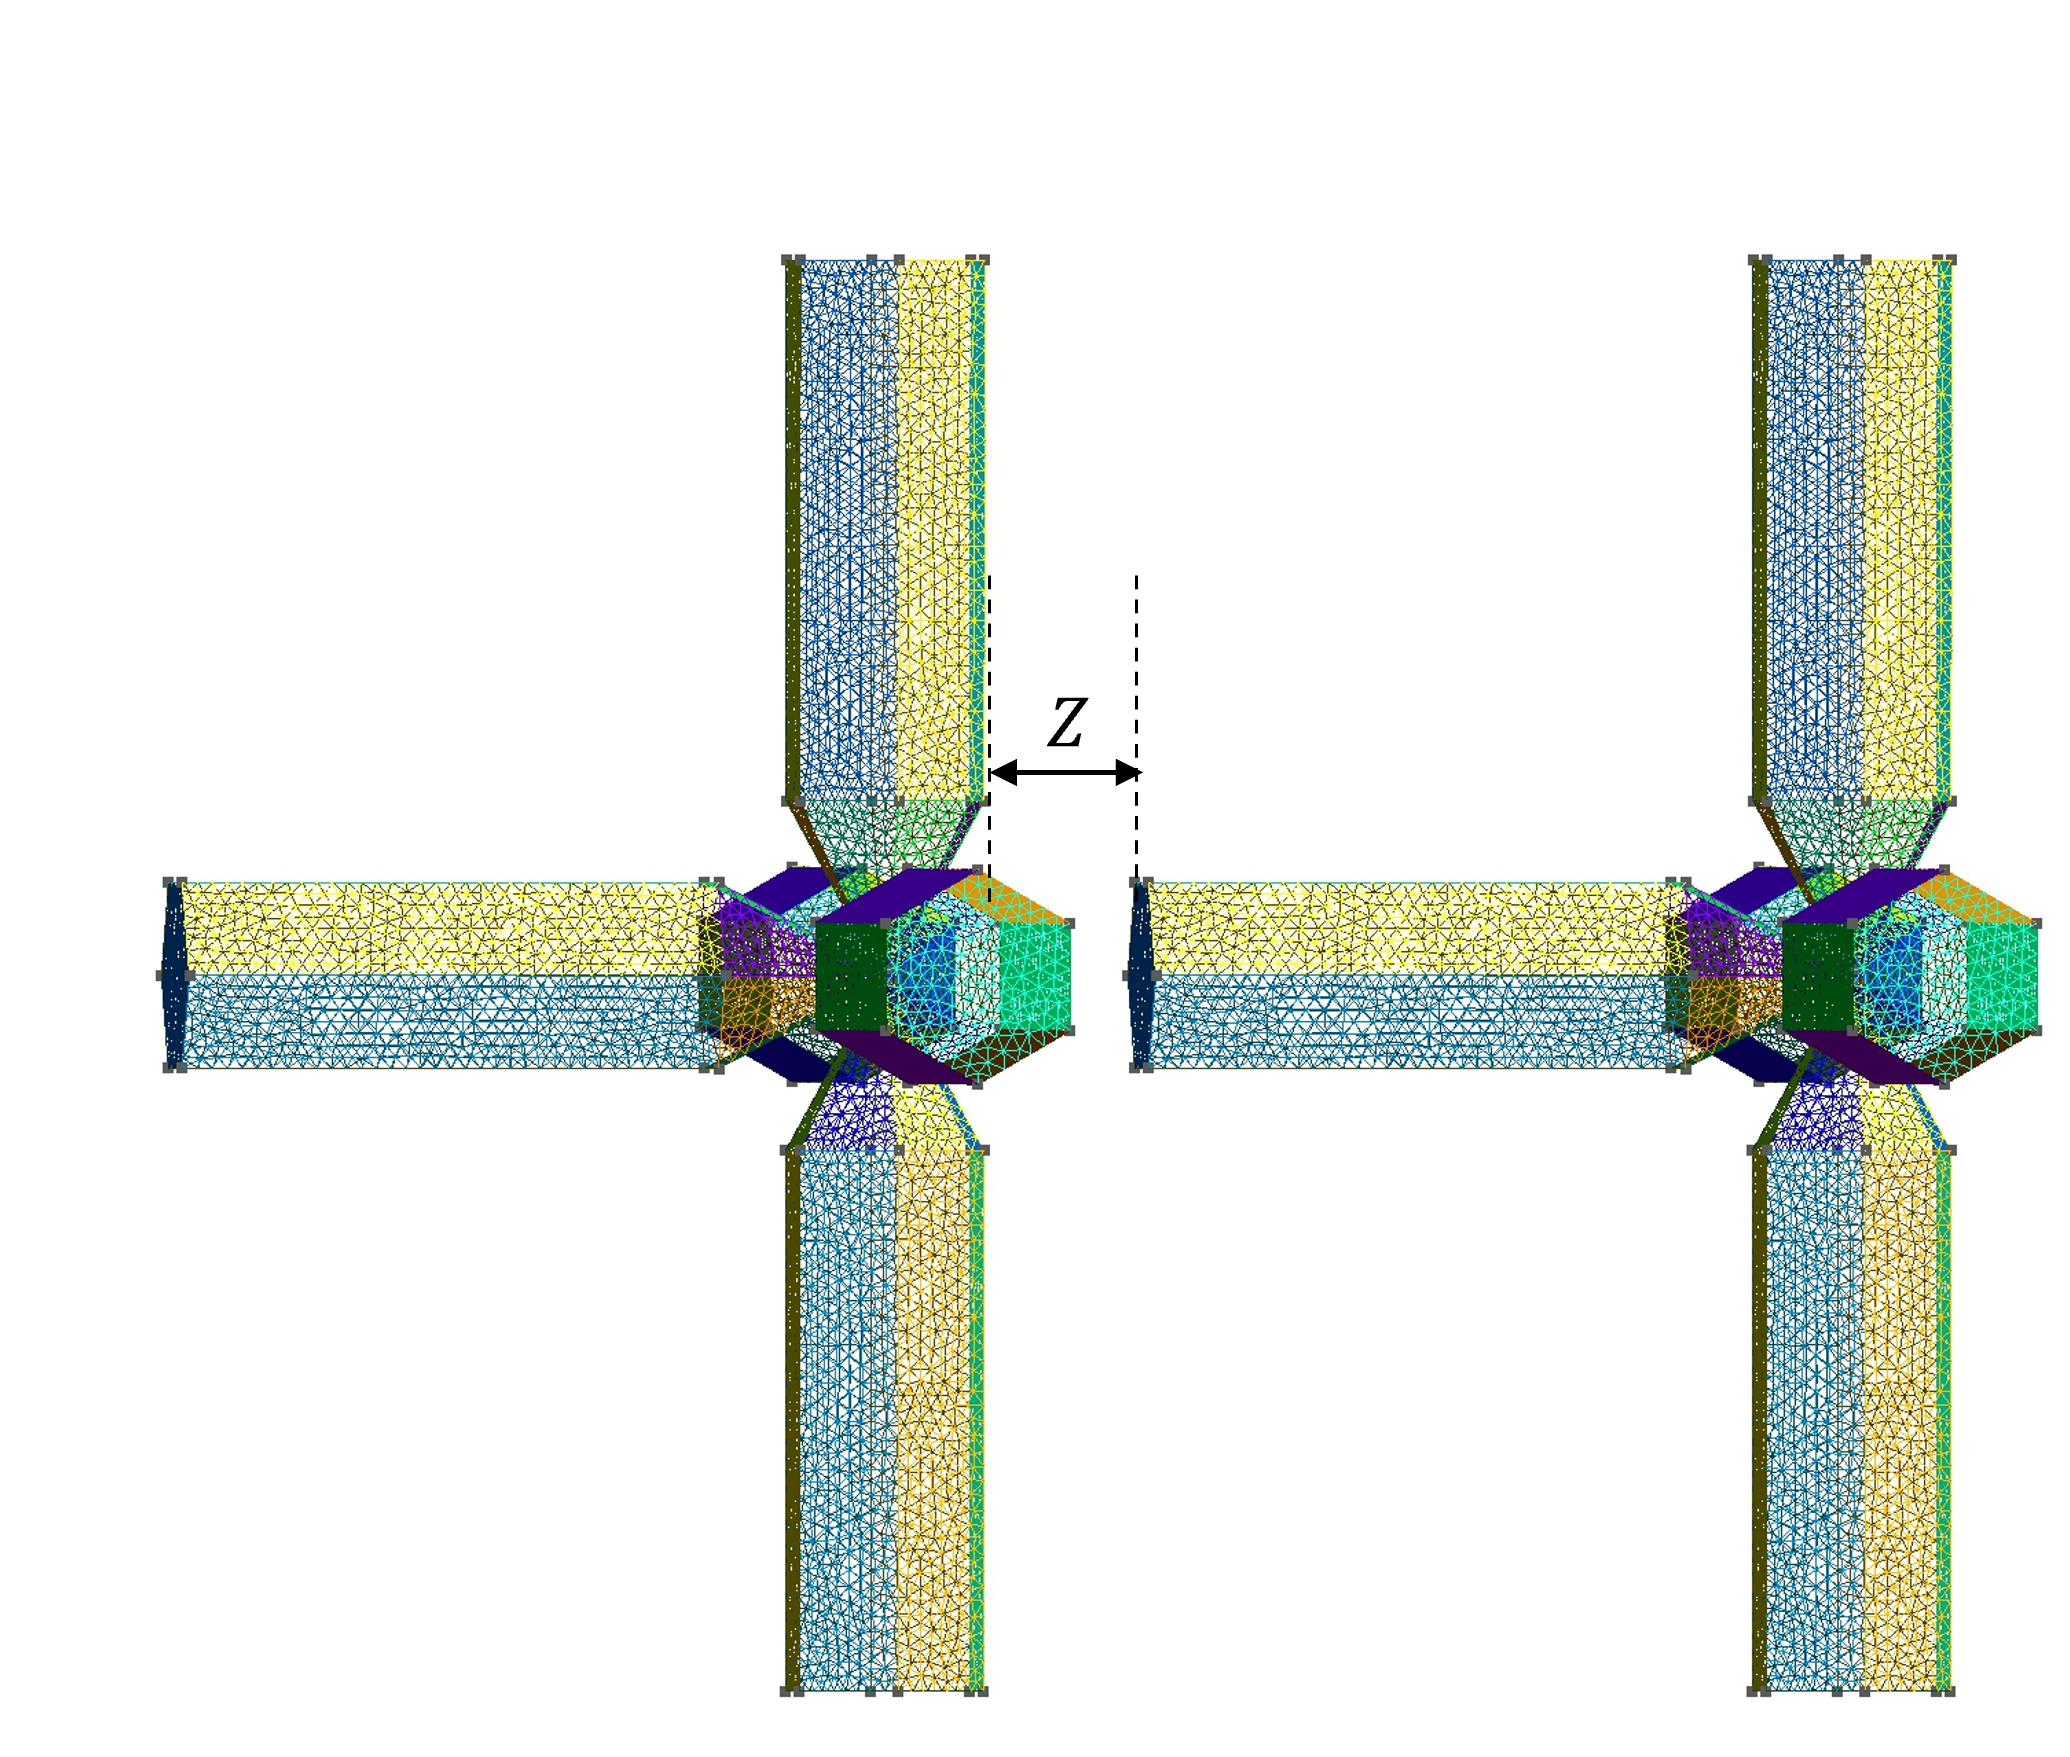
\includegraphics[scale = 0.4]{figures/5branches}
    \caption{Five branches}
    \end{subfigure}%
    \begin{subfigure}{.5\linewidth}
    \centering
    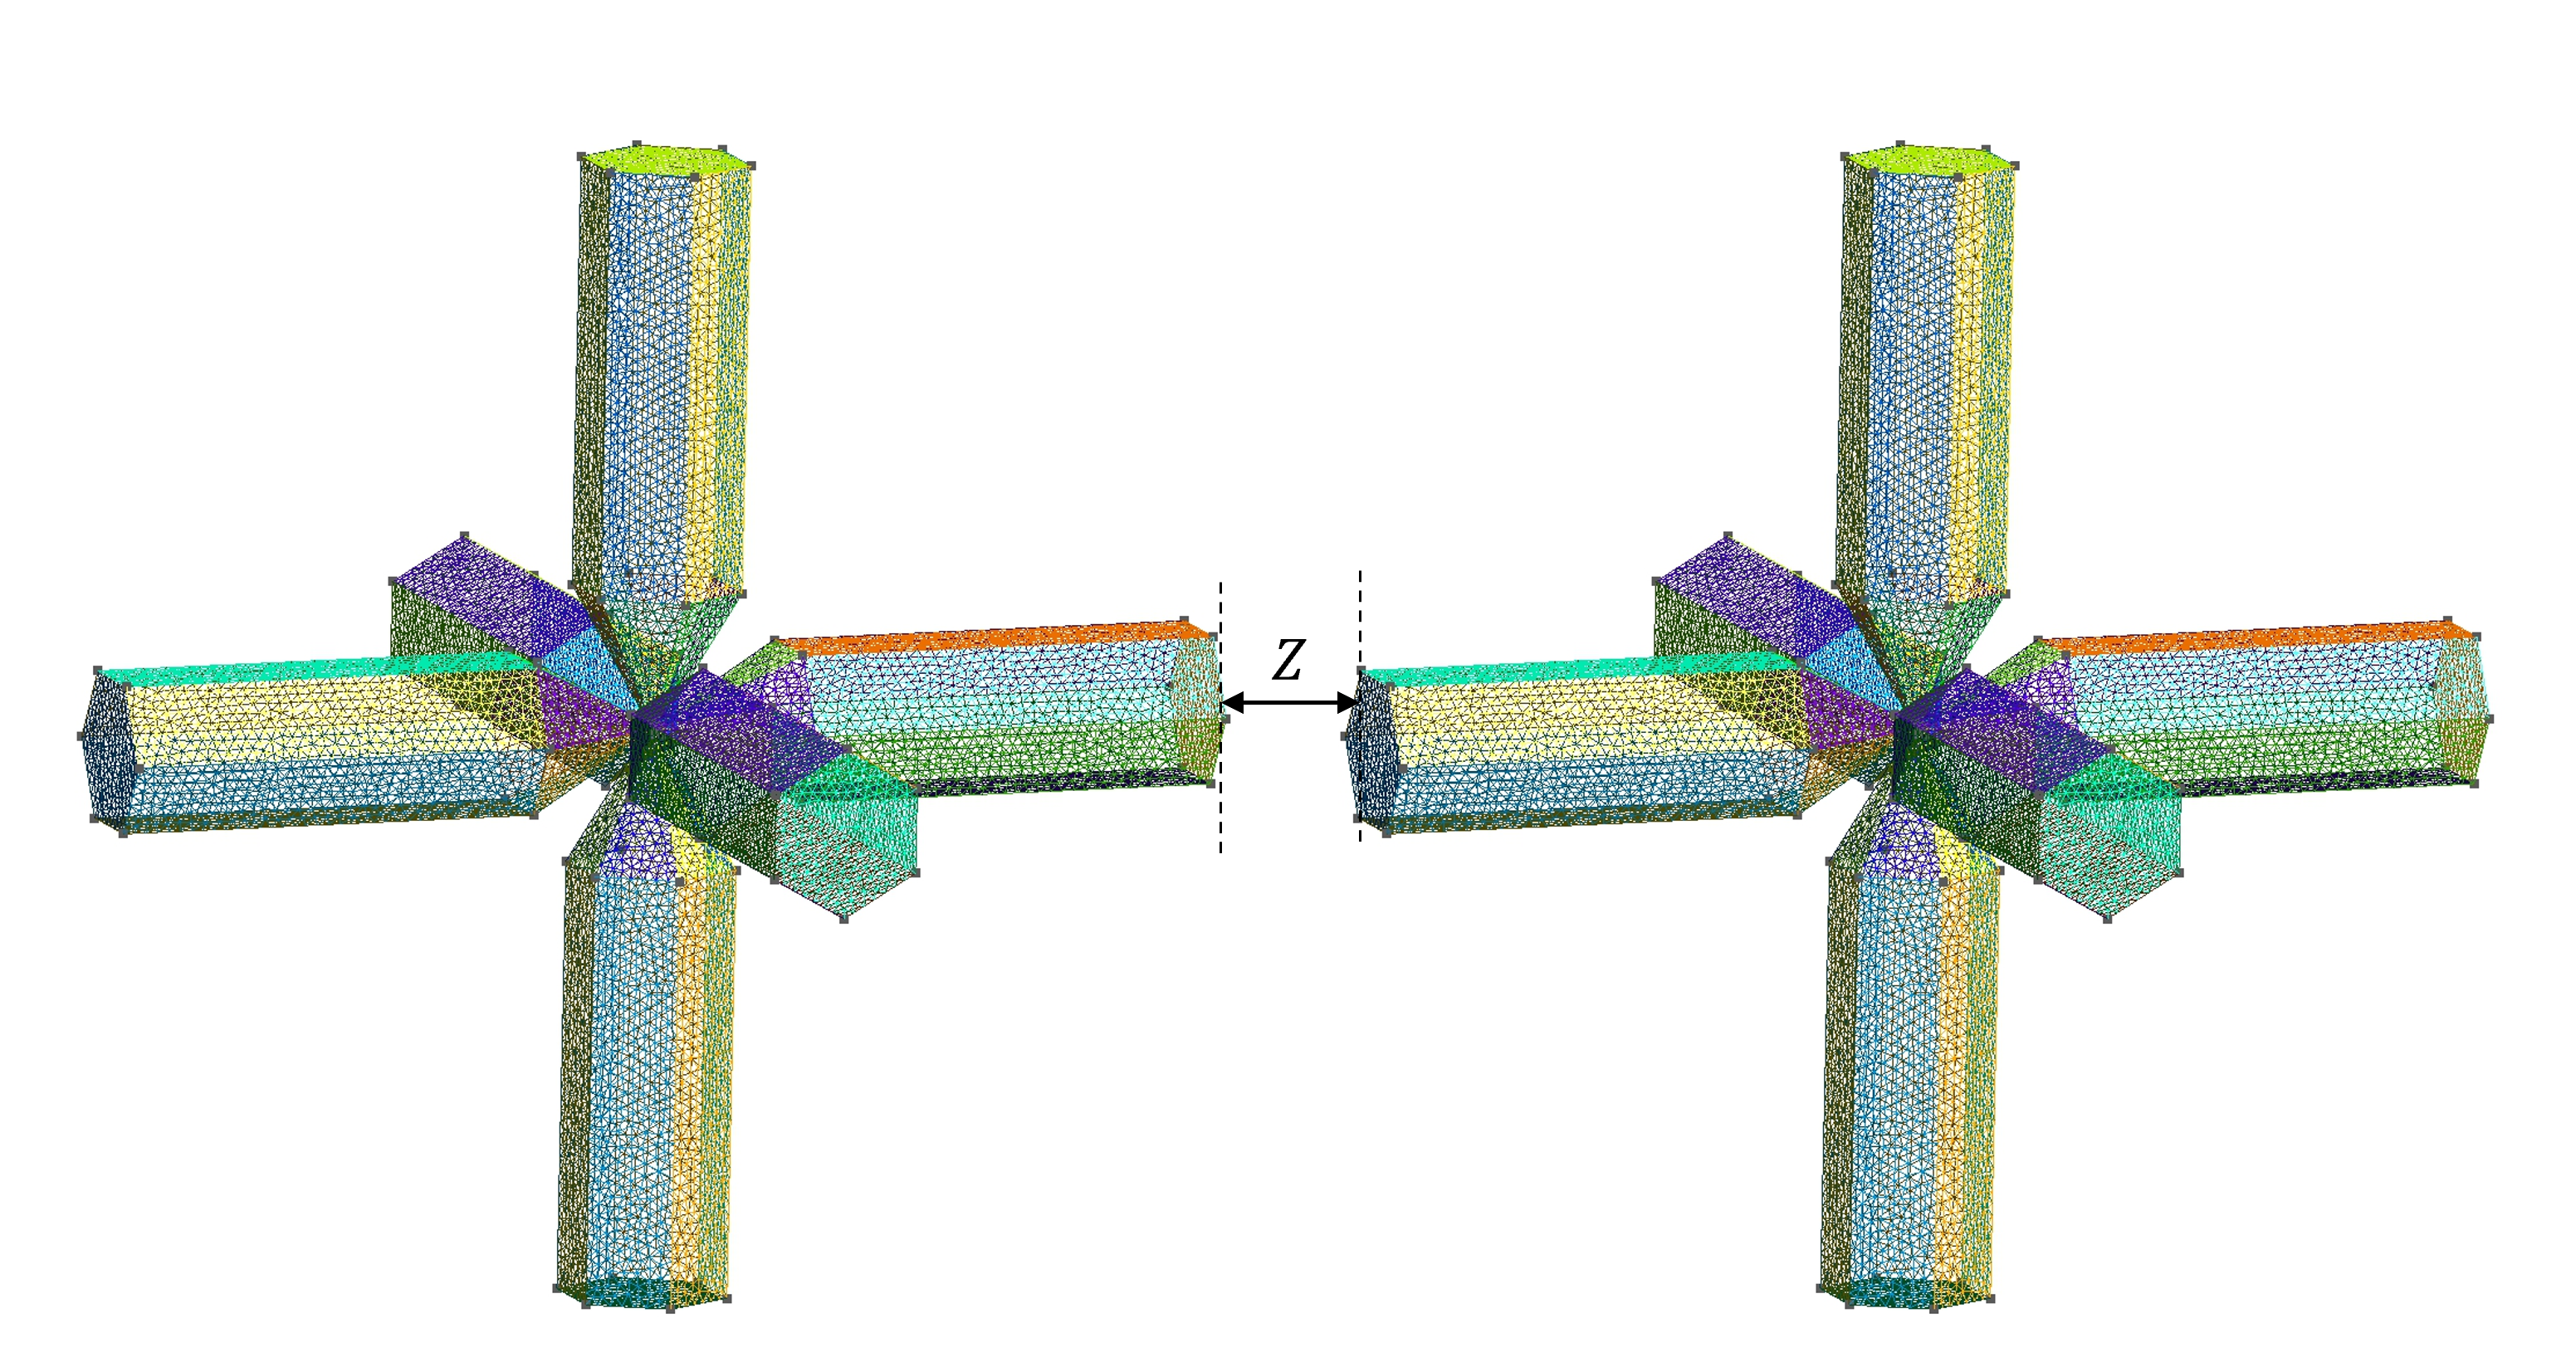
\includegraphics[scale = 0.4]{figures/6branches}
    \caption{Six branches}
    \end{subfigure}
    \caption{Ice crystals with different number of branches}
    \label{Ice crystals with different number of branches}
    \end{figure}

    \begin{figure}[H]
        \centering
        \hspace*{-1cm}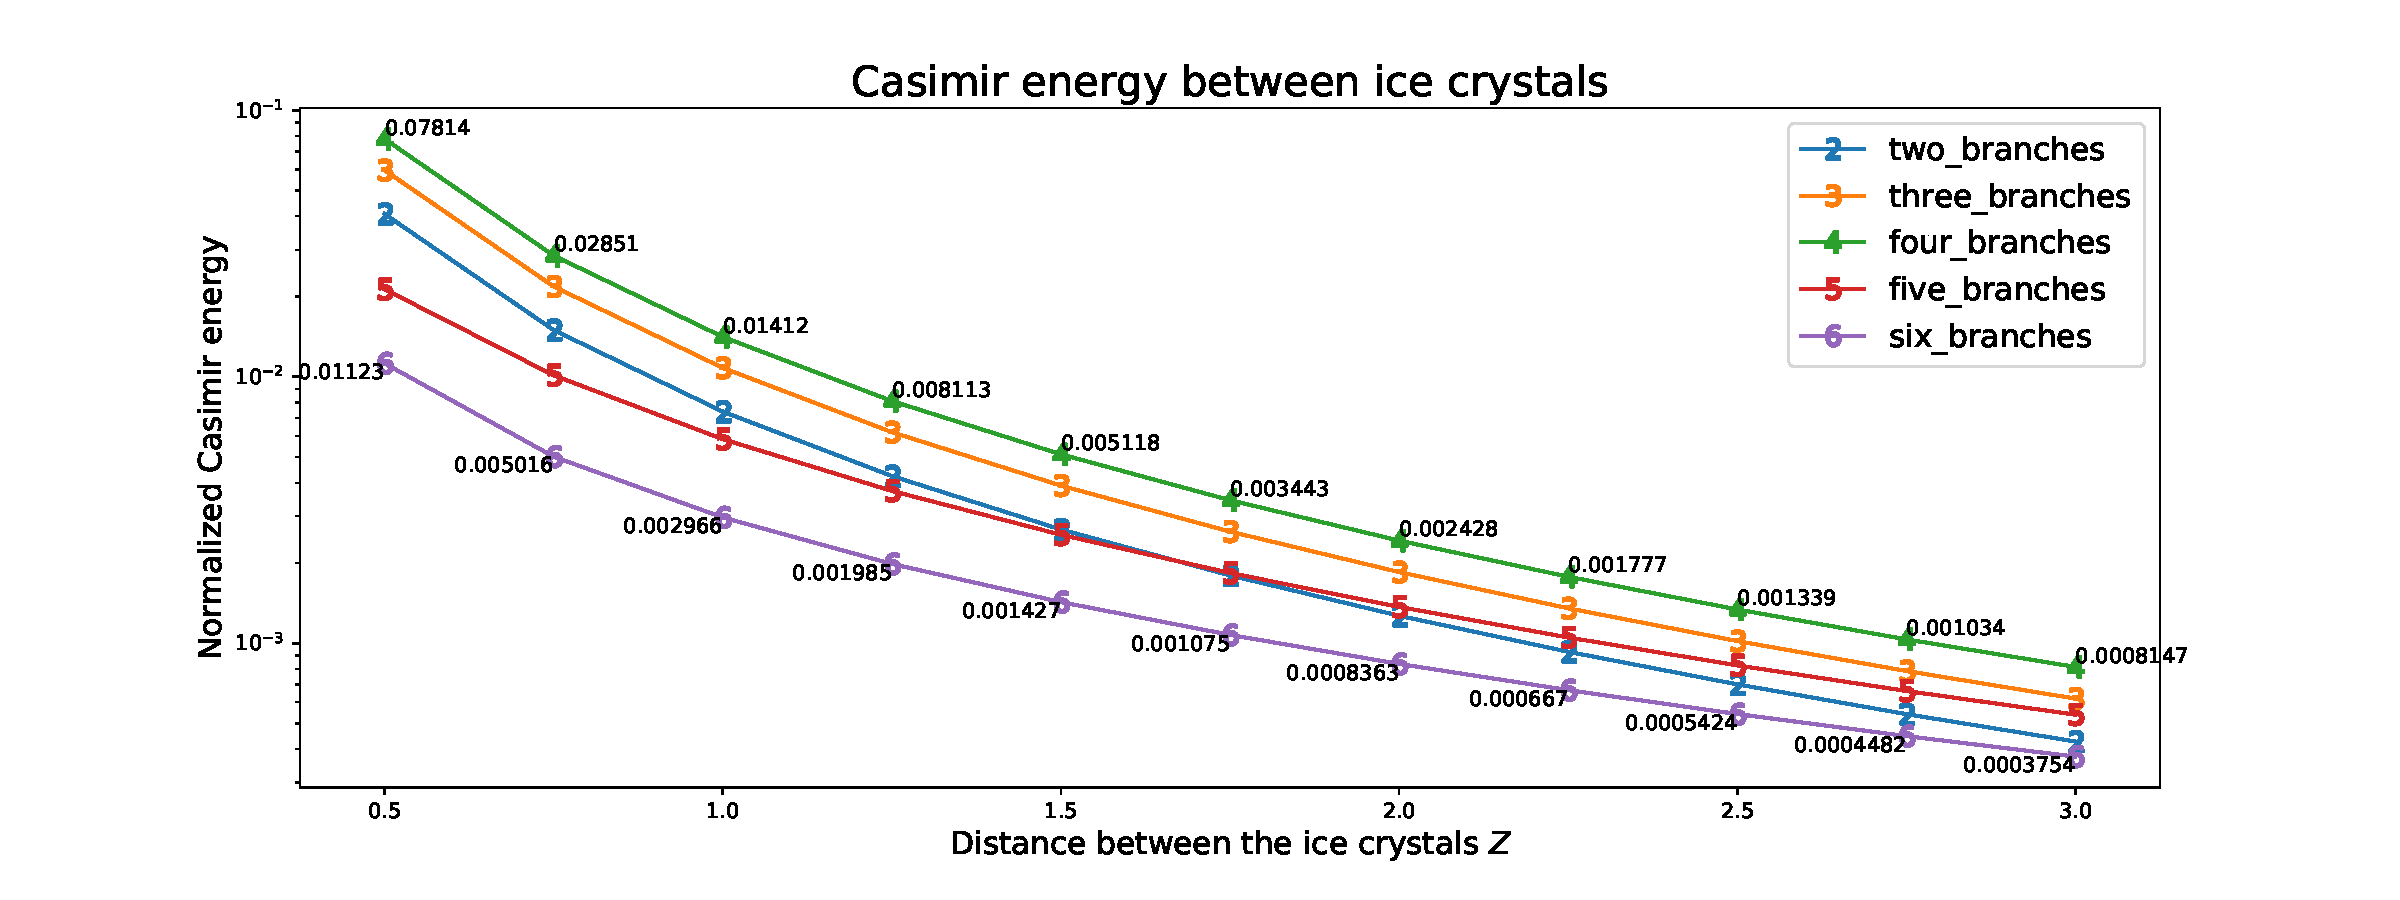
\includegraphics[scale = 0.5]{figures/CasE_ice_crystals.pdf}
        \caption{Normalized Casimir energy in ice crystals' case. To make the figure keep clear, only the 4-branches and 6-branches's case data points 
        are labelled in the figure.}
        \label{Normalized Casimir energy in ice crystals' case}
    \end{figure}
%==================================================================================================


It is not hard to imagine that the Casimir energy would be different after the scatterers rotate while keeping the distance between them unchanged. Therefore, 
in the last example, we would see how the Casimir energy between two identical ellipsoids changes as one of the ellipsoids rotates.

In Figure \ref{Without rotation}, the above ellipsoid is centering at $(0,0,0)$ and 
the points $(0.5, 0, 0), (0, 1, 0)$ and $(0, 0, 0.5)$ are located on this surface and if the distance between these two ellipsoids is denoted as $Z$, then the below one
is centering at $(0, 0, -(0.5+0.5+Z))$ and the points $(0.5, 0, -(0.5+0.5+Z)), (0, 1, -(0.5+0.5+Z))$ and $(0, 0, 0.5-(0.5+0.5+Z))$ are on it. Without rotation, 
the Casimir energy between them with different distance $Z$ is plotted in Figure \ref{Casimir energy between two ellipsoids with different distances}.

To explore how the rotation affects the change of the Casimir energy, one can always keep one ellipsoid fixed and rotate the other one. The Figure 
\ref{Rotation around z-axis} and \ref{Rotation around x-axis} describe the case when one of the ellipsoids rotates around $z-$ and $x-$axis, respectively.
From the Figure \ref{Casimir energy when one of the ellipsoids rotates}, the Casimir energy changes periodically since we rotate one ellipsoid around 
$z-$ or $x-$ axis by 360 degrees. 


\begin{figure}[H]
    \begin{subfigure}{\linewidth}
        \centering
        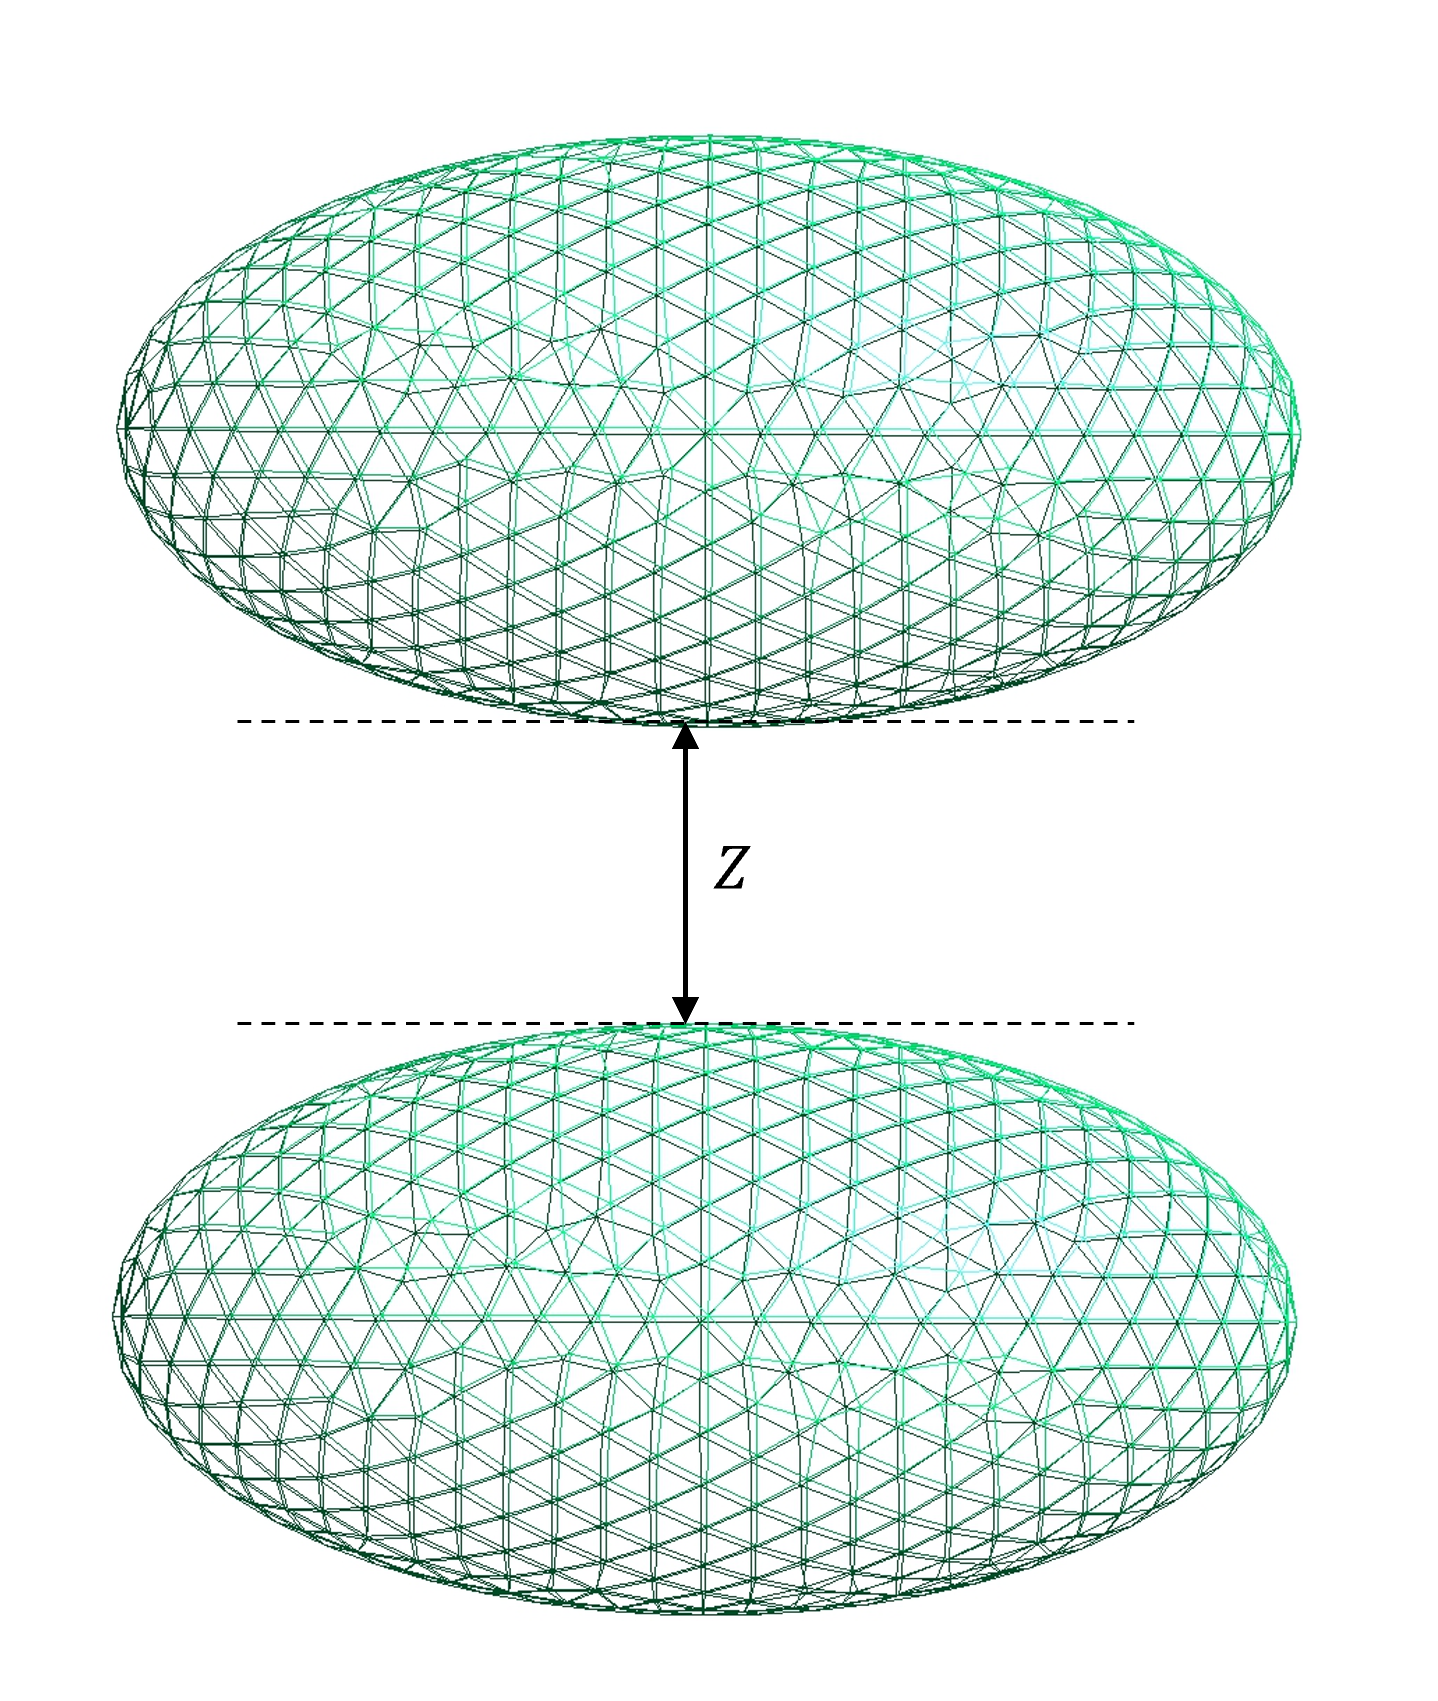
\includegraphics[scale = 0.4]{figures/two_ellipsoids}
        \caption{Without rotation}
        \label{Without rotation}
        \end{subfigure}\\[1ex]
    \begin{subfigure}{.5\linewidth}
    \centering
    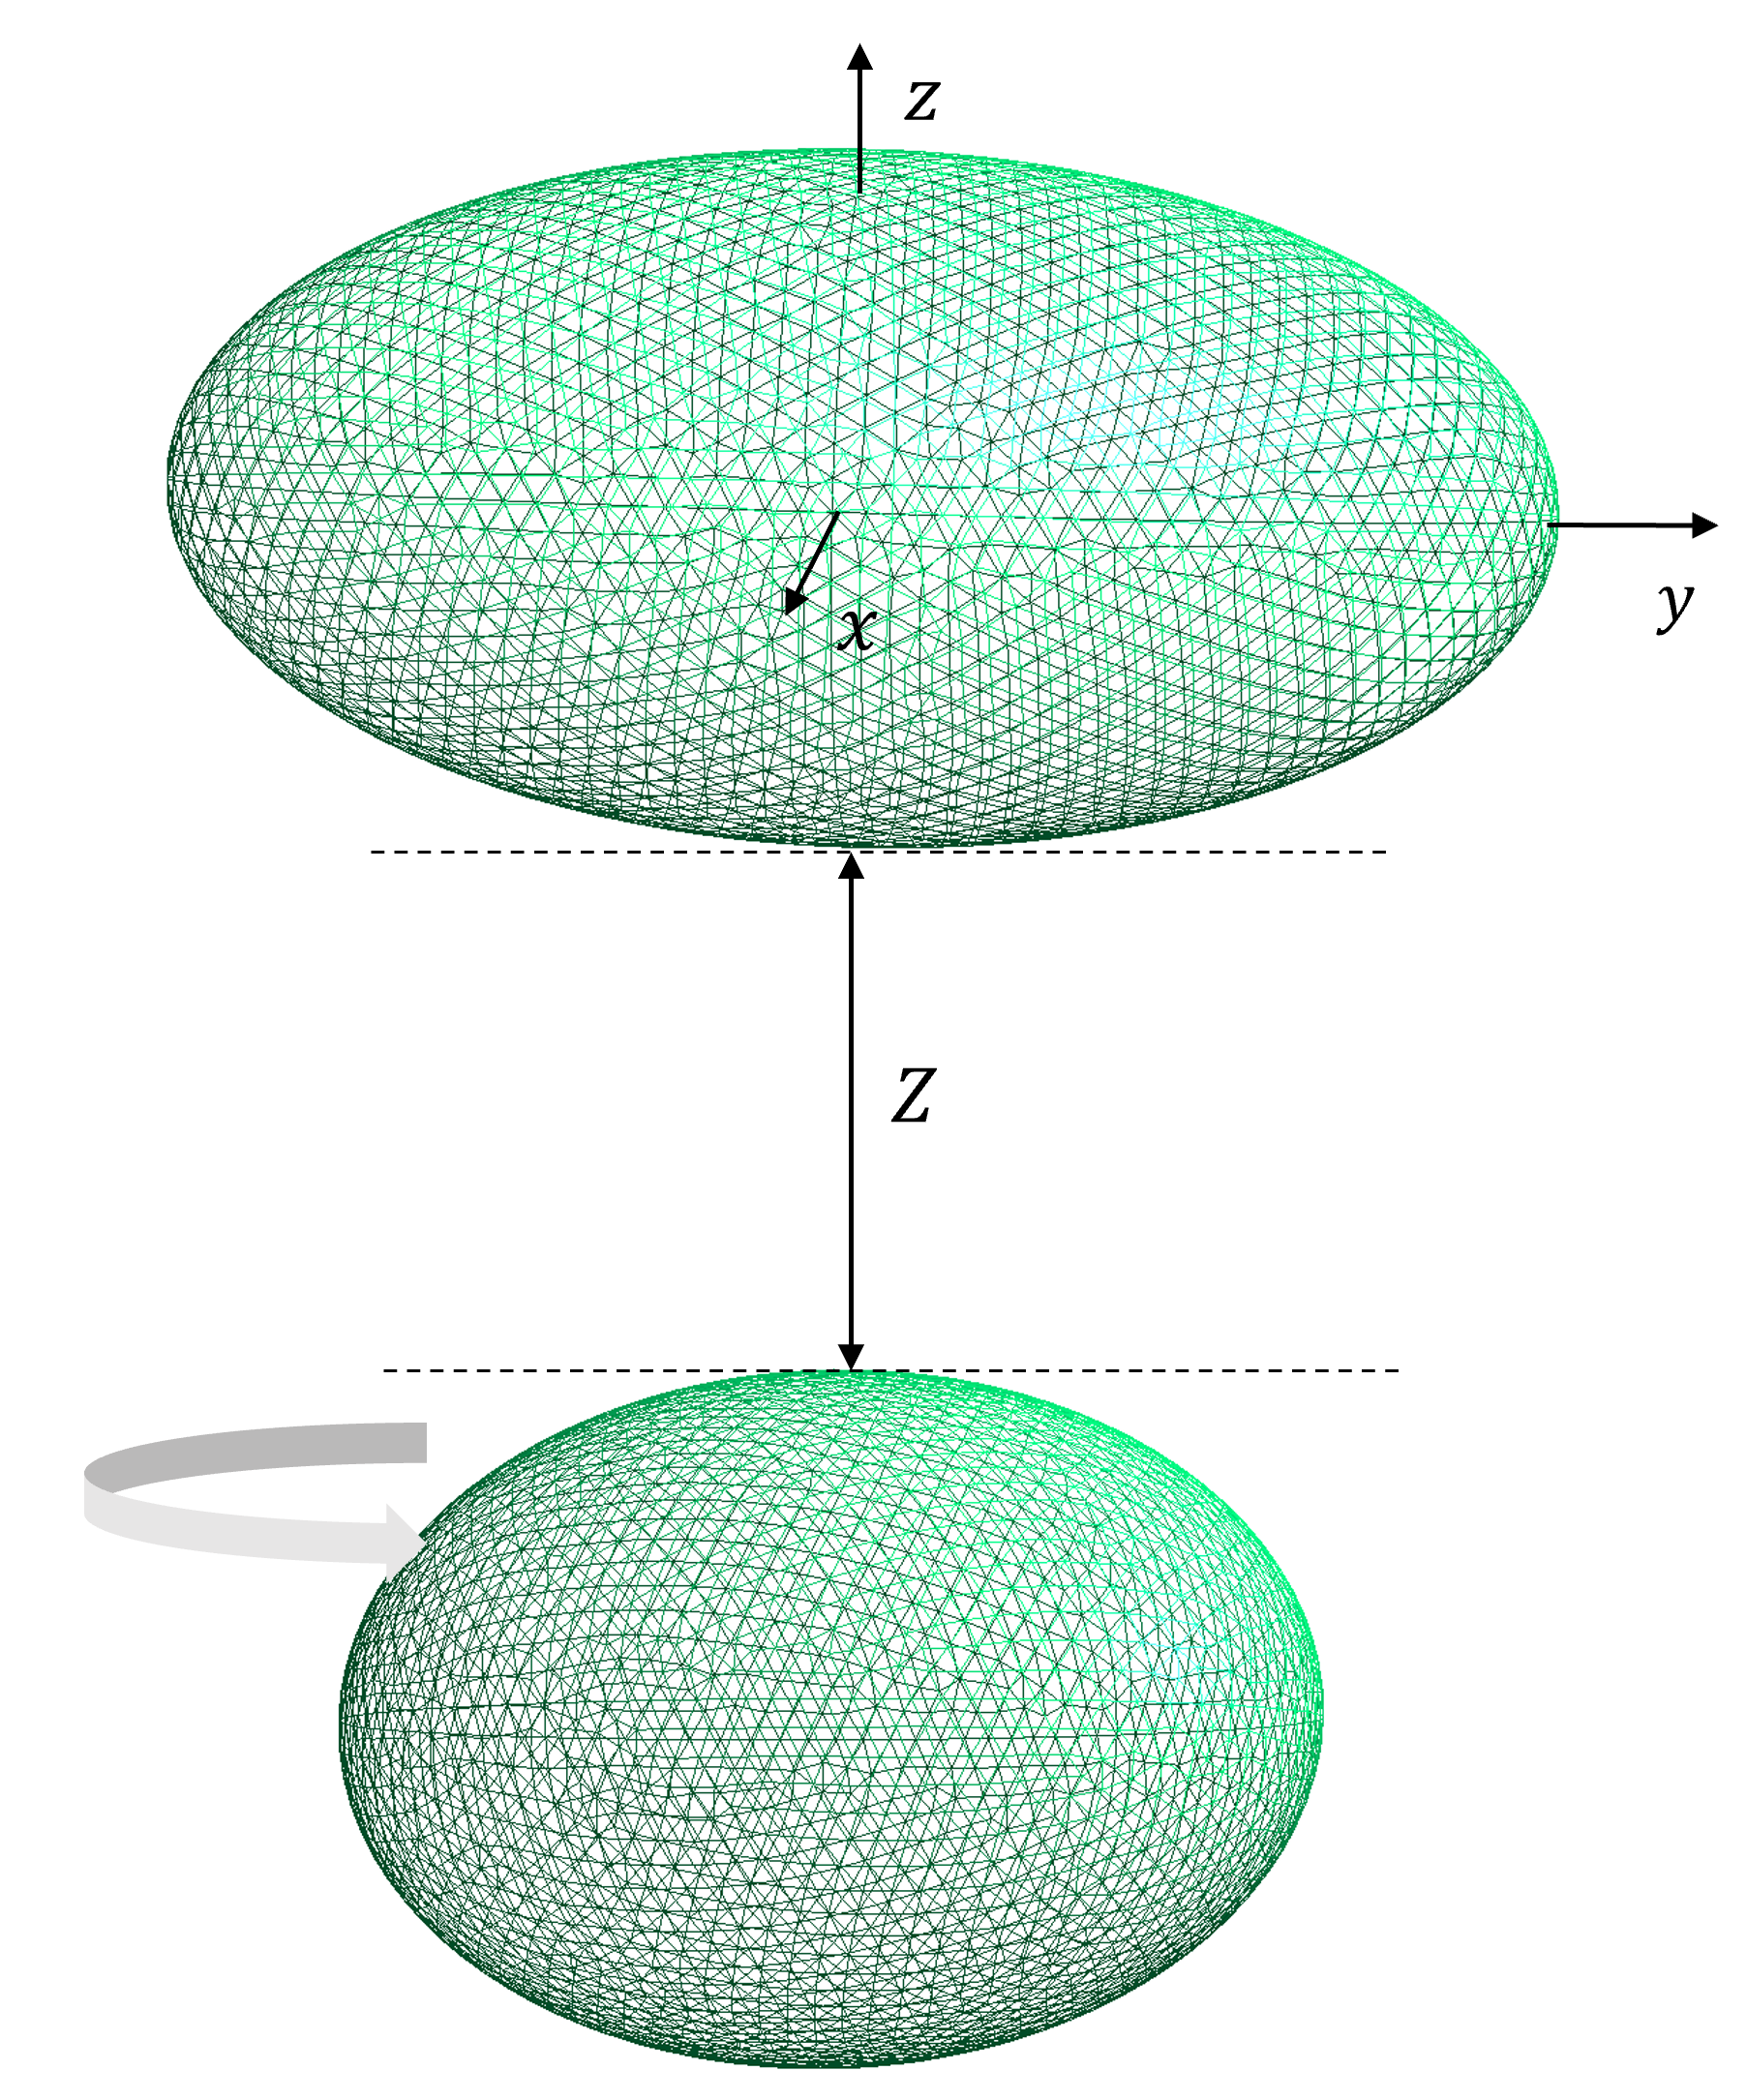
\includegraphics[scale = 0.4]{figures/Ellipsoid_z_axis}
    \caption{Rotation around z-axis}
    \label{Rotation around z-axis}
    \end{subfigure}%
    \begin{subfigure}{.5\linewidth}
    \centering
    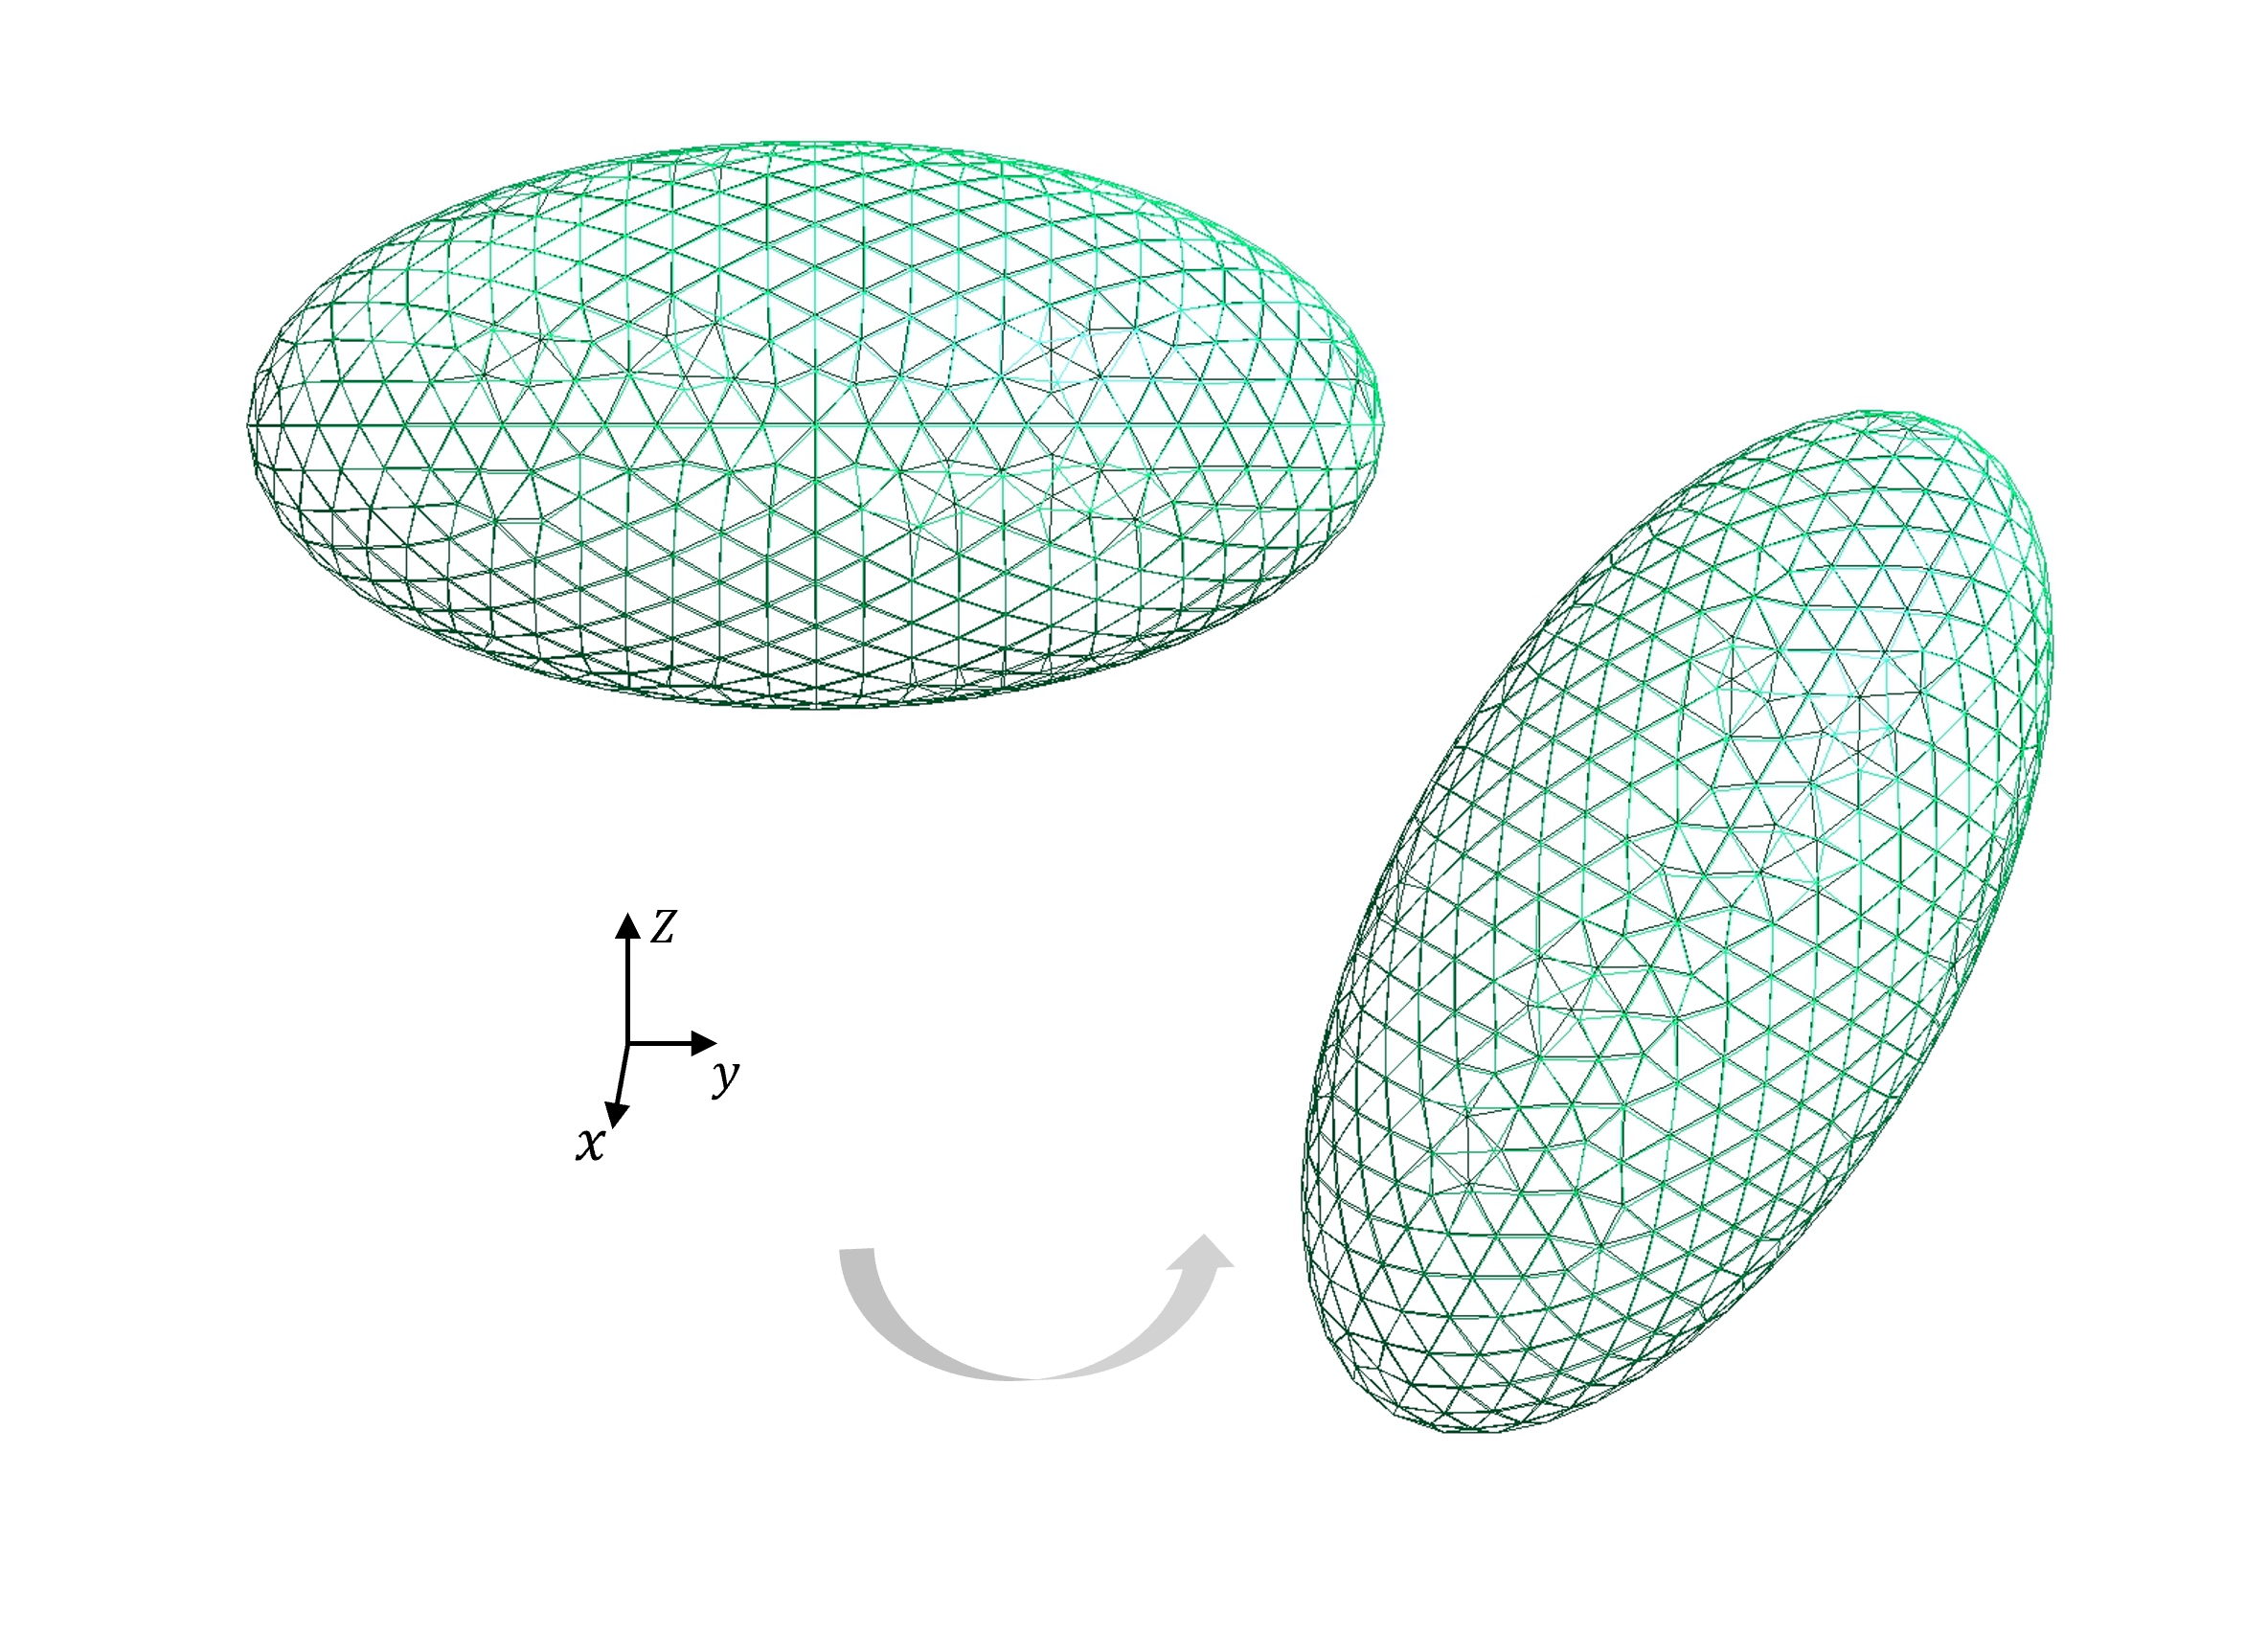
\includegraphics[scale = 0.4]{figures/Ellipsoid_x_axis}
    \caption{Rotation around x-axis}
    \label{Rotation around x-axis}
    \end{subfigure}
    \caption{Two ellipsoids with or without rotation}
    \label{Two ellipsoids}
    \end{figure}

    \begin{figure}[H]
        \begin{subfigure}{\linewidth}
            \centering
            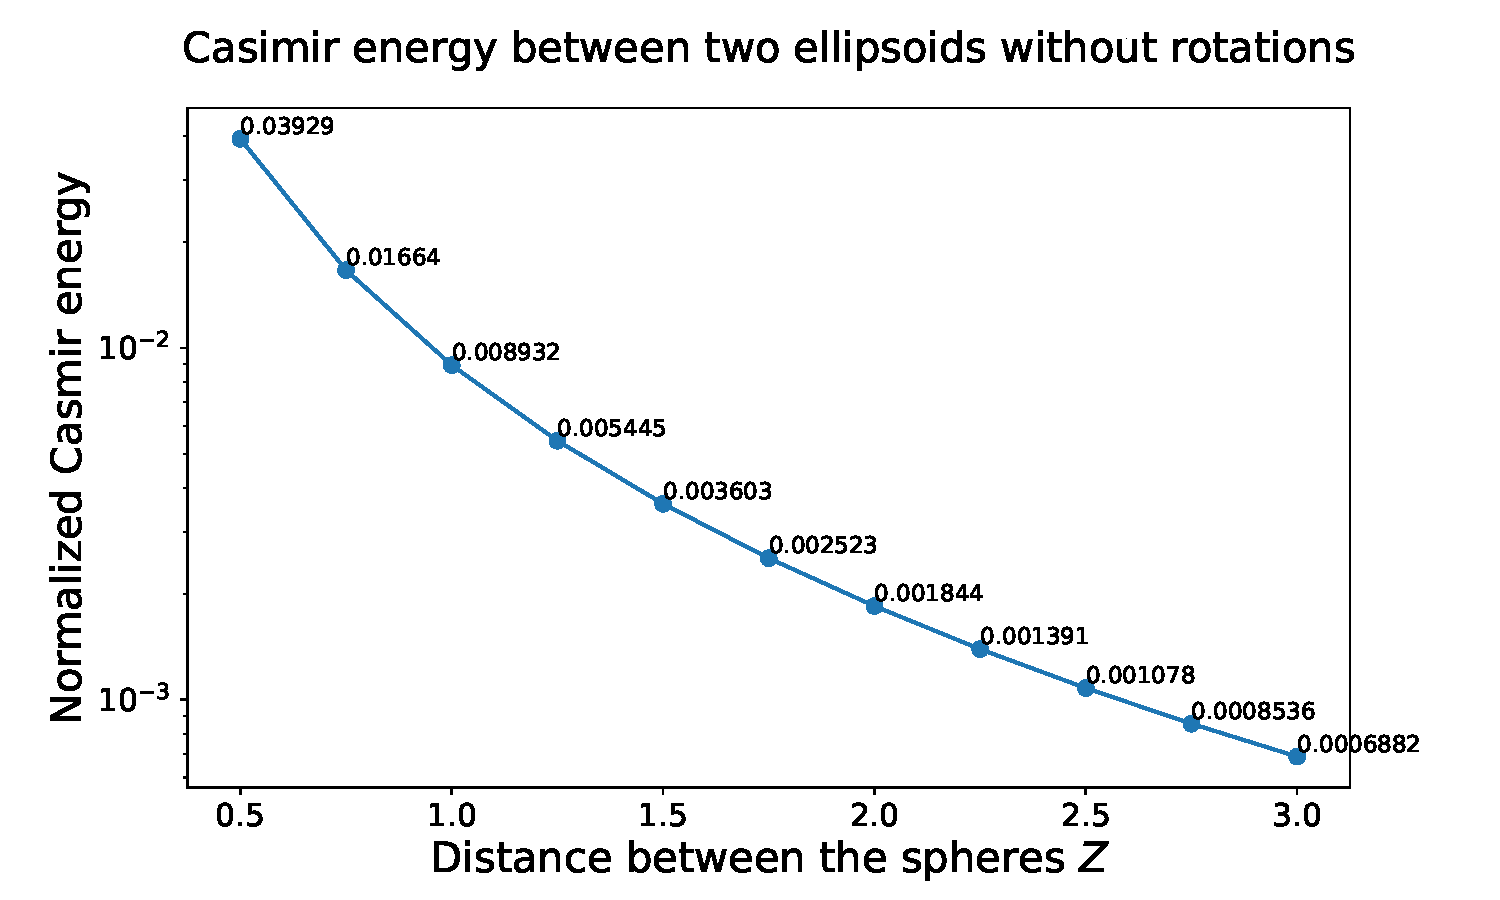
\includegraphics[scale = 0.5]{figures/CasE_ellipsoids.pdf}
            \caption{Casimir energy between two ellipsoids with different distances}
            \label{Casimir energy between two ellipsoids with different distances}
            \end{subfigure}\\[1ex]
    
        \begin{subfigure}{\linewidth}
        \centering
        \hspace*{-1cm}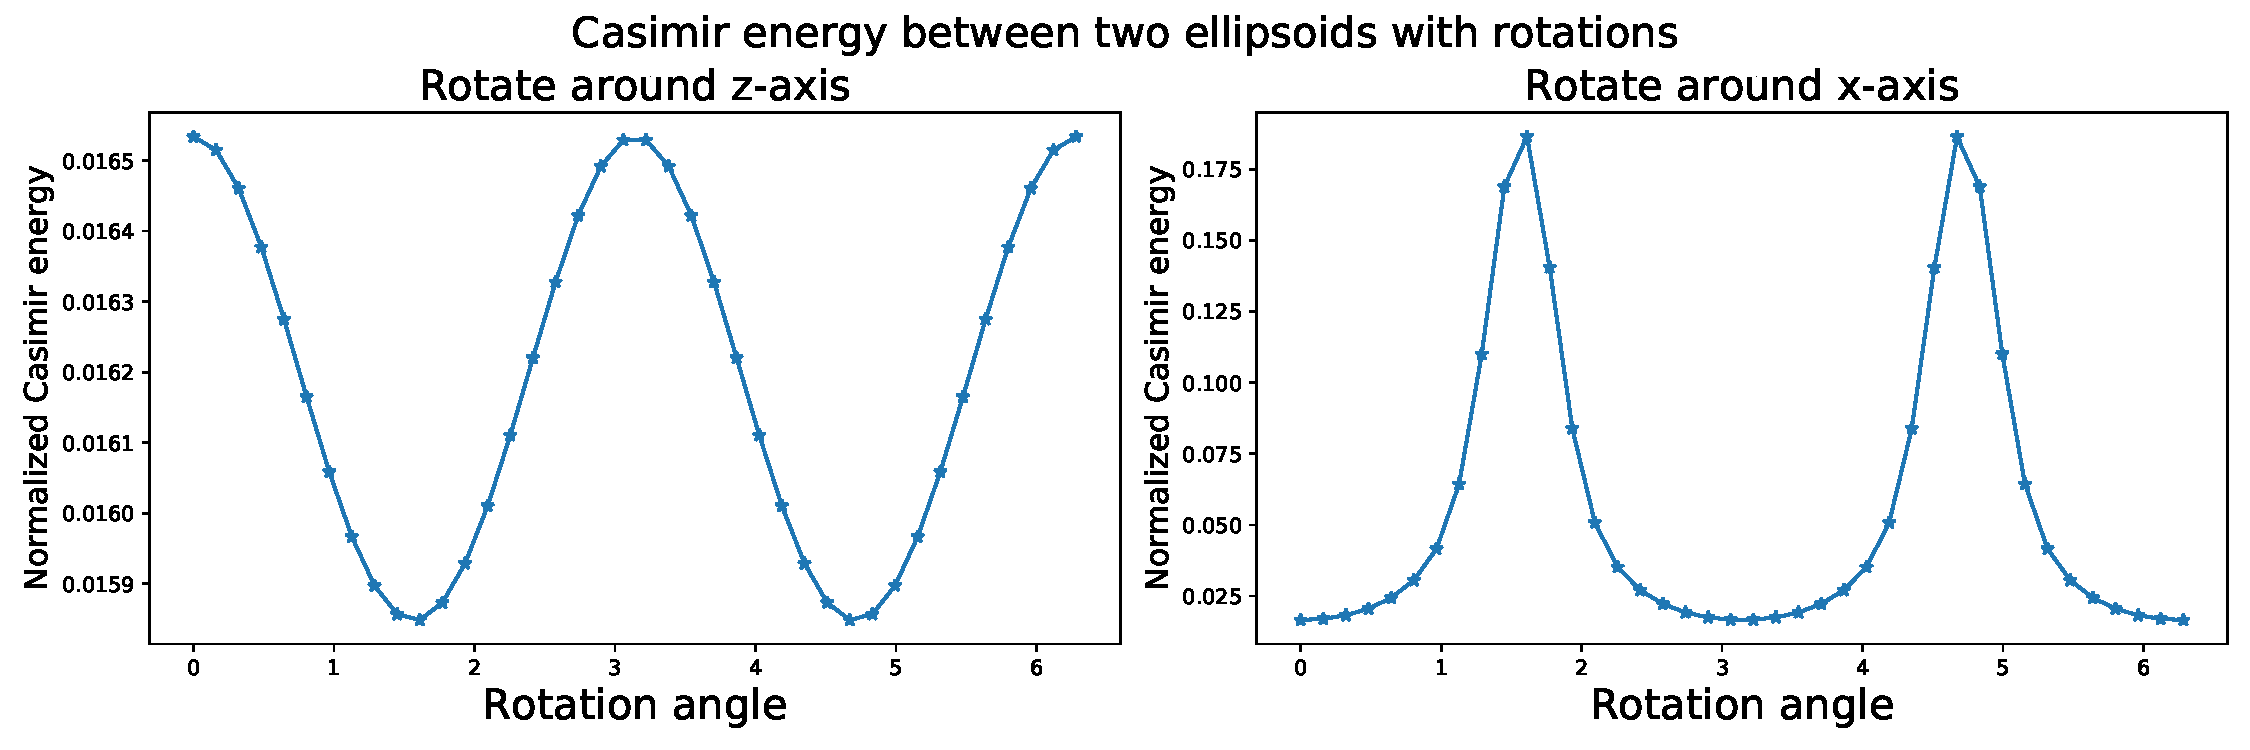
\includegraphics[scale = 0.5]{figures/CasE_ellipsoids_with_rotation.pdf}
        \caption{Casimir energy when one of the ellipsoids rotates}
        \label{Casimir energy when one of the ellipsoids rotates}
        \end{subfigure}
        \caption{The dependence of the Casimir energy and rotation angle of one of the ellipsoids.} 
        \end{figure}



\section{Conclusion}\label{Conclusion}
The determinant formula for the Casimir energy in terms of boundary layer operators provides a good and accurate approach to its numerical computation.
We have demonstrated that modern methods from computational linear algebra combined with the idea of subspace recycling can provide a significant 
speedup and accuracy boost in computations of Casimir forces and energies.


%\section{Bibliography styles}
% \cite{Feynman1963118}.

\section*{References}

\bibliography{mybibfile_}

\end{document}